\section{Cumulative Sum with Controlled Memory Layout and Skew}
\label{sec:memorylayout}
In this section, we describe our attempt to improve the query times for the wavelet tree by controlling the memory layout and skewing the tree.
Skewing the tree means that we force it to be unbalanced with a bias to one side. 
Brodal et al.~\citeA{gerthSkewedBinarySearchTrees} showed that skewing a binary search tree could reduce the amount of cache misses and branch mispredictions considerately. Enough, in fact, to increase the speed of searching the tree manyfold, even though the skewing increased the depth of the tree structure.

To reduce cache misses by skewing the tree we must control the memory layout, because by skewing the tree to the right, we increase the likelihood of a traversal similar to a depth-first-search going down the right side first (DFSr). So we want to place the data in memory so that a DFSr traversal through the tree would result in sequential address accesses.
Allocating memory dynamically as we go might produce a similar layout and controlling the memory may not lead to increased performance, but it is the only way to ensure the memory layout is as we want it.

Skewing the tree has the disadvantage of increasing the height, or depth, of the tree.
J.~Nievergelt and E.~M. Reingold~\citeB{Nievergelt:1972:BST:800152.804906} defined the height for a skewed binary tree to be at most:
\[ h_{max} = \frac{\log(m+1)}{ \log\frac{1}{1-\alpha}} \;,\]
where $m$ is the total number of nodes in the tree, that is $2 \sigma - 1$ in our wavelet tree, and $\alpha = \frac{1}{\mathit{skew}}$ and \textit{skew} is the number that is divided by to skew our tree, see Section~\ref{sec:SkewingTheTree}.
Together this makes the height at most
\[ h_{max} = \frac{\log(2 \sigma)}{ \log\frac{\mathit{skew}}{\mathit{skew} - 1}}  \;.\]
Which, when the tree is balanced, so $\mathit{skew} = 2$, makes the height at most $h_{max} = \log \sigma + 1$ which agrees with our definition of the height $h = \lceil \log \sigma \rceil$.

Let us analyse the theoretical worst case running time of constructing and querying a balanced wavelet tree vs. a skewed wavelet tree.

Constructing a balanced wavelet tree takes  $O(n \cdot \log \sigma)$ time because the height of the tree is $\lceil \log \sigma \rceil$ and there are $n$ elements in each level.
When skewing the tree the height of the tree becomes as defined above and the construction time becomes $O(n \cdot h_{max})$.

The query time for rank on a balanced wavelet tree is $O(b \log \sigma)$ and for select $O(b \log \sigma + \log \frac{n}{b} \log \sigma)$.
In the skewed version of the tree the rank query time then becomes worst-case $O(b \cdot h_{max})$. The query time for select becomes $O(b \cdot h_{max} + \log \frac{n}{b} \cdot~h_{max})$.
The memory usage becomes $O(n \cdot h_{max} + \sigma + \frac{n}{b} \cdot h_{max})$.


From the theoretical analysis of construction time and query time of a skewed wavelet tree it is theoretically not an improvement to skew the tree.
Skewing the tree can however reduce branch mispredictions, as shown by Brodal et al.~\citeA[Abstract]{gerthSkewedBinarySearchTrees}.
It does so by giving the branch in the direction the tree is skewed a much higher probability of being the correct than the other, which enables the branch prediction unit to predict correctly more often. 
Skewing the tree can also reduce cache misses by increasing the probability that the next piece of memory the algorithm accesses is already loaded into a cacheline by the time it is accessed because of prefetching.

The algorithms for construction and queries in this implementation remain mostly the same as before in CumulativeSum, but with modifications to handle a controlled memory layout and a skew of the tree.

\subsection{Prefetching}
Prefetching is a feature of the CPU whereby it can fetch other parts of the memory into cachelines even though it was not requested yet, if it expects it will be requested soon, to avoid having the program waiting for this fetching.
In more advanced versions, it can even look at the access into memory of the running program and try to determine a pattern and prefetch memory according to this pattern.
Looking at the Intel Optimization Manual~\citeB{intel-optimization-manual} for our architecture\footnote{Our architecture is Ivy Bridge, but the optimization manual sections for Sandy Bridge holds true for Ivy Bridge as well, as stated in section 2.2.7 in~\citeB{intel-optimization-manual}.} we find that it has streaming prefetchers loading into L1, L2, and last level cache. The streaming prefetchers detect accesses to ascending or descending addresses and can prefetch up to 20 lines ahead or behind. 
Our architecture also has a prefetcher that can detect strides in memory access, as well as a “Next Page Prefetcher” that can load another memory page when detecting memory accesses near the page boundary~\footnote{See section 2.2.7 of~\citeB{intel-optimization-manual}}.


\subsection{Skewing The Tree}
\label{sec:SkewingTheTree}
Skewing the tree is done by changing the way we find which character in the alphabet to split on in each node's construction.
The split character is the last character in the alphabet of the left child node and to be able to skew the calculation we calculate it as
\[\mathit{SplitCharacter} = \left\lfloor \frac{\mathit{alphabetSize}-1}{\mathit{skew}} + \mathit{alphabetMin} \right\rfloor \]
where \textit{alphabetSize} is the size of the alphabet at this node, \textit{alphabetMin} is the first character in the alphabet at this node, and \textit{skew} is the skew parameter which is 2 for a balanced tree and higher for right-skewed trees. E.g. a \textit{skew} value of 4 skews the tree by 75\,\% to the right so that, in each node, 25\,\% of the alphabet is put into the left child node and 75\,\% is put into the right child node.
We only use integer values as characters, so the calculated split character is rounded down.


\subsection{Controlled Memory Layout}
We still want to support dynamic input and alphabet sizes without recompilation, so the nodes must be dynamically allocated on the heap.

The size of a node is known at compile time as it contains fixed-size pointers to the parent node and left and right child nodes, as well as a boolean to flag it as a leaf node and its bitmap as a vector, which internally stores a pointer to its backing array.
As such, the memory for the nodes is allocated by allocating an array and then instantiating the nodes into that array.
A reference to a pointer is passed into the array from parent to child nodes during construction, so they know where to allocate their child nodes.
The pointer points to the position of the last node in the array, and so before each instantiation of a new node, we increment the pointer so it points to free space, then place the new node there.

The memory layout of the bitmaps are not controlled, because skewing the tree will not help the prefetcher with regards to the bitmaps, except in a few specific cases, because of the way the bitmaps are used and the resulting access patterns.
The algorithms for rank and select stop querying each bitmap at some position inside the bitmap and then continue to the next bitmap in the next node.
Rank stops when it reaches the position the query was searching up to, given as a parameter.
Select stops when it has found the sought number of occurrences in the bitmap.
In both these cases the rest of the bitmap is not used and any such data the prefetcher has fetched would have been in vain.
The prefetcher cannot tell from the algorithms access pattern when it will jump ahead to the next bitmap, and every such jump will therefore give rise to a cache miss.
The problem is shown in Figure~\ref{fig:QueryPrefetchFigure}. The drawing assumes the bitmap is stored sequentially and the prefetcher prefetches the next cache line (colored green), but the algorithm stops at some position and skips ahead to the next bitmap. 
This makes it unable to utilize the prefetched data and will try to access memory that is not in the cache yet; a cache miss.
So regardless of where the bitmap that is accessed next is stored, following right after the first or elsewhere in memory, a cache miss will occur.

The exceptions to this are when either the entire bitmap is used for the query, that is, when the rank query is for the entire string, or the bitmap is small enough that the beginning of the next bitmap can fit within the same word.
The first case is not a common query in most use cases, and the second case is rare when the input string is much bigger than the alphabet, and would only happen near the leaf nodes.
Neither scenario happens often enough to warrant controlling the bitmap memory layouts.

\begin{figure}\tiny
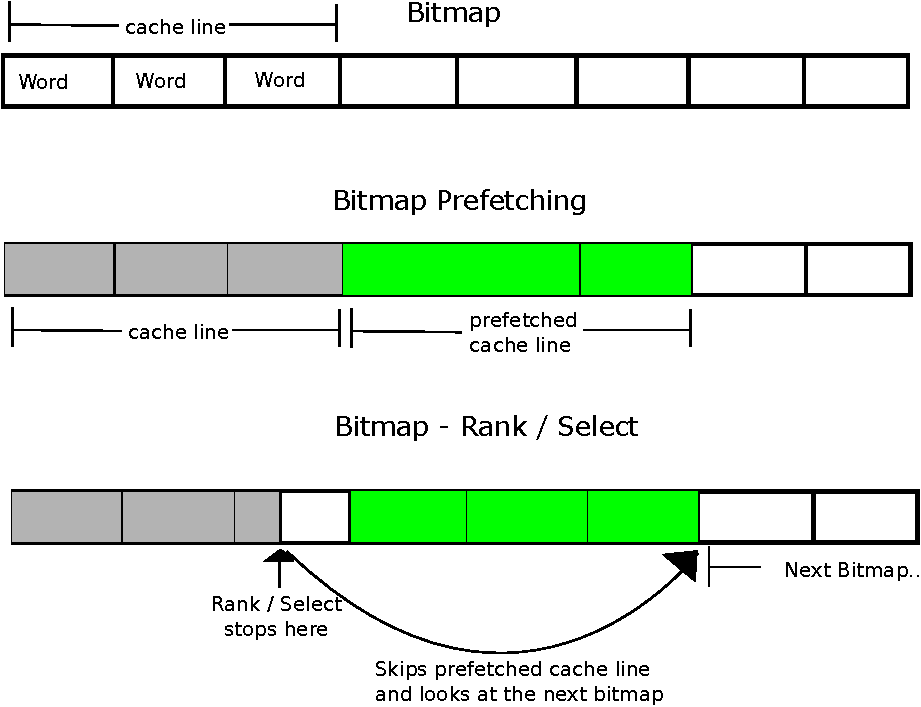
\includegraphics[width=\textwidth]{QueryPrefetchFigure.pdf}
\caption{How access patterns in a concatenated bitmap can defeat cache prefetching}
\label{fig:QueryPrefetchFigure}
\end{figure}



\subsection{Experiments}

\subsubsection{Queries when skewing the Wavelet Tree using uncontrolled and controlled memory layout}
In this experiment we want to test whether queries on a skewed tree using controlled memory layout is an improvement in running time.

\paragraph{Test Setup}~\\
The general setup is as described in Section~\ref{sec:ExpNotesGeneralSetup}.
The query parameters were chosen as described in Section~\ref{sec:choiceOfQueryParameters}.
The results can be seen in Figure~\ref{fig:CumulativeSumSkew_n8as16_Build}, Figure~\ref{fig:CumulativeSumSkew_n8as16_Rank} and Figure~\ref{fig:CumulativeSumSkew_n8as16_Select}.
We skew the wavelet tree as described in Section~\ref{sec:SkewingTheTree}).
The block size used for testing the build time and memory usage is 1024, as we found that to be the overall best when weighing both rank and select time and memory usage.
The block size used for rank is 64 bit and 2048 bit for select, as that gave the best performance for each, and we wanted to give each the best possibility to perform well when skewed.
The less time that is spent in binary rank and binary select, the greater the influence on running time of branch mispredictions and cache misses from navigation nodes in the tree, and therefore the better opportunity for reducing these has to improve running time.

\paragraph{Results}~\\
Looking at Figure~\ref{fig:CumulativeSumSkew_n8as16_Build_WallTime}, we can see that it takes more time to build a skewed tree, with increasing time spent as the skew increases.
It appears to be a linear increase in running time as skew increases, especially from skew parameter 3 and higher.
Looking at Figure~\ref{fig:CumulativeSumSkew_n8as16_build_memory} we can see that it also takes more memory the more we skew the tree.
If we look at Figure~\ref{fig:CumulativeSumSkew_n8as16_Rank} and Figure~\ref{fig:CumulativeSumSkew_n8as16_Select} we can see that query times for both rank and select also increase linearly with increasing skew.

We can already conclude that skewing the tree is not worth it in terms of build time, memory usage \textit{or} query times.
We still look closer at our measurements and try to explain why it is not worth it.

Looking at Figure~\ref{fig:CumulativeSumSkew_n8as16_Rank_CM} and Figure~\ref{fig:CumulativeSumSkew_n8as16_Select_CM} we can see the amount of cache misses increases as skew increases for both rank and select queries and for all three levels of cache.
If we instead look at level 2 data cache \textit{hits} in Figure~\ref{fig:CumulativeSumSkew_n8as16_Rank_L2CH} and Figure~\ref{fig:CumulativeSumSkew_n8as16_Select_L2CH}, we can see that they in fact increase as well, and at a higher rate than the cache misses, which is also what the rising cache hit rate signifies.
The high increase in level 2 data cache hits is no benefit, however, when level 2 data cache misses still increase, as it is the misses that cause a penalty and no increased amount of cache hits can make up for that penalty.

In Figure~\ref{fig:CumulativeSumSkew_n8as16_Rank_BMExe} and Figure~\ref{fig:CumulativeSumSkew_n8as16_Select_BMExe} we see an increase branches executed, which is to be expected, as the depth of the tree increases, more nodes must be traversed using branching code.
While more branches are taken overall, we also see in Figure~\ref{fig:CumulativeSumSkew_n8as16_Rank_BM} and Figure~\ref{fig:CumulativeSumSkew_n8as16_Select_BM} a reduction in both the amount of branch mispredictions and the branch misprediction rate as the tree is skewed further.
The reduction in the raw amount of branch mispredictions leads directly to a reduction in performance penalties incurred, but the increase in total number of conditional branches executed might not be worth it.
The amount of branches executed at skew factor 6 compared to skew factor 2 (balanced) increases by 37,149 for rank and 1,365,427 for select, whereas the amount of branch mispredictions are only reduced by 1,377 for rank and 63,116 for select, meaning that there is 21 additional branches per branch misprediction saved for rank and 27 for select.
A branch misprediction penalty must then be at least either 21 or 27 cpu cycles before it would be worth it in terms branch mispredictions, assuming a single branch instruction takes one cpu cycle.

Figure~\ref{fig:CumulativeSumSkew_n8as16_Rank_TLBM} and Figure~\ref{fig:CumulativeSumSkew_n8as16_Select_TLBM} show the amount of Translation Lookaside Buffer Misses encountered as the tree is skewed.
While it has higher variation and both dips and rises the more the tree is skewed, it does still show a general increase at higher skew parameter values.

\begin{figure}\tiny
\begin{subfigure}{0.48\textwidth}
	% GNUPLOT: LaTeX picture with Postscript
\begingroup
  \makeatletter
  \providecommand\color[2][]{%
    \GenericError{(gnuplot) \space\space\space\@spaces}{%
      Package color not loaded in conjunction with
      terminal option `colourtext'%
    }{See the gnuplot documentation for explanation.%
    }{Either use 'blacktext' in gnuplot or load the package
      color.sty in LaTeX.}%
    \renewcommand\color[2][]{}%
  }%
  \providecommand\includegraphics[2][]{%
    \GenericError{(gnuplot) \space\space\space\@spaces}{%
      Package graphicx or graphics not loaded%
    }{See the gnuplot documentation for explanation.%
    }{The gnuplot epslatex terminal needs graphicx.sty or graphics.sty.}%
    \renewcommand\includegraphics[2][]{}%
  }%
  \providecommand\rotatebox[2]{#2}%
  \@ifundefined{ifGPcolor}{%
    \newif\ifGPcolor
    \GPcolortrue
  }{}%
  \@ifundefined{ifGPblacktext}{%
    \newif\ifGPblacktext
    \GPblacktexttrue
  }{}%
  % define a \g@addto@macro without @ in the name:
  \let\gplgaddtomacro\g@addto@macro
  % define empty templates for all commands taking text:
  \gdef\gplbacktext{}%
  \gdef\gplfronttext{}%
  \makeatother
  \ifGPblacktext
    % no textcolor at all
    \def\colorrgb#1{}%
    \def\colorgray#1{}%
  \else
    % gray or color?
    \ifGPcolor
      \def\colorrgb#1{\color[rgb]{#1}}%
      \def\colorgray#1{\color[gray]{#1}}%
      \expandafter\def\csname LTw\endcsname{\color{white}}%
      \expandafter\def\csname LTb\endcsname{\color{black}}%
      \expandafter\def\csname LTa\endcsname{\color{black}}%
      \expandafter\def\csname LT0\endcsname{\color[rgb]{1,0,0}}%
      \expandafter\def\csname LT1\endcsname{\color[rgb]{0,1,0}}%
      \expandafter\def\csname LT2\endcsname{\color[rgb]{0,0,1}}%
      \expandafter\def\csname LT3\endcsname{\color[rgb]{1,0,1}}%
      \expandafter\def\csname LT4\endcsname{\color[rgb]{0,1,1}}%
      \expandafter\def\csname LT5\endcsname{\color[rgb]{1,1,0}}%
      \expandafter\def\csname LT6\endcsname{\color[rgb]{0,0,0}}%
      \expandafter\def\csname LT7\endcsname{\color[rgb]{1,0.3,0}}%
      \expandafter\def\csname LT8\endcsname{\color[rgb]{0.5,0.5,0.5}}%
    \else
      % gray
      \def\colorrgb#1{\color{black}}%
      \def\colorgray#1{\color[gray]{#1}}%
      \expandafter\def\csname LTw\endcsname{\color{white}}%
      \expandafter\def\csname LTb\endcsname{\color{black}}%
      \expandafter\def\csname LTa\endcsname{\color{black}}%
      \expandafter\def\csname LT0\endcsname{\color{black}}%
      \expandafter\def\csname LT1\endcsname{\color{black}}%
      \expandafter\def\csname LT2\endcsname{\color{black}}%
      \expandafter\def\csname LT3\endcsname{\color{black}}%
      \expandafter\def\csname LT4\endcsname{\color{black}}%
      \expandafter\def\csname LT5\endcsname{\color{black}}%
      \expandafter\def\csname LT6\endcsname{\color{black}}%
      \expandafter\def\csname LT7\endcsname{\color{black}}%
      \expandafter\def\csname LT8\endcsname{\color{black}}%
    \fi
  \fi
  \setlength{\unitlength}{0.0500bp}%
  \begin{picture}(4608.00,3600.00)%
    \gplgaddtomacro\gplbacktext{%
      \csname LTb\endcsname%
      \put(444,384){\makebox(0,0)[r]{\strut{} 0}}%
      \put(444,691){\makebox(0,0)[r]{\strut{} 2}}%
      \put(444,998){\makebox(0,0)[r]{\strut{} 4}}%
      \put(444,1305){\makebox(0,0)[r]{\strut{} 6}}%
      \put(444,1612){\makebox(0,0)[r]{\strut{} 8}}%
      \put(444,1920){\makebox(0,0)[r]{\strut{} 10}}%
      \put(444,2227){\makebox(0,0)[r]{\strut{} 12}}%
      \put(444,2534){\makebox(0,0)[r]{\strut{} 14}}%
      \put(444,2841){\makebox(0,0)[r]{\strut{} 16}}%
      \put(444,3148){\makebox(0,0)[r]{\strut{} 18}}%
      \put(444,3455){\makebox(0,0)[r]{\strut{} 20}}%
      \put(608,264){\makebox(0,0){\strut{} 2}}%
      \put(1070,264){\makebox(0,0){\strut{} 2.5}}%
      \put(1531,264){\makebox(0,0){\strut{} 3}}%
      \put(1992,264){\makebox(0,0){\strut{} 3.5}}%
      \put(2454,264){\makebox(0,0){\strut{} 4}}%
      \put(2915,264){\makebox(0,0){\strut{} 4.5}}%
      \put(3376,264){\makebox(0,0){\strut{} 5}}%
      \put(3837,264){\makebox(0,0){\strut{} 5.5}}%
      \put(4299,264){\makebox(0,0){\strut{} 6}}%
      \put(96,1919){\rotatebox{-270}{\makebox(0,0){\strut{}Wall Time (seconds)}}}%
      \put(2453,84){\makebox(0,0){\strut{}Skew Parameter}}%
    }%
    \gplgaddtomacro\gplfronttext{%
    }%
    \gplbacktext
    \put(0,0){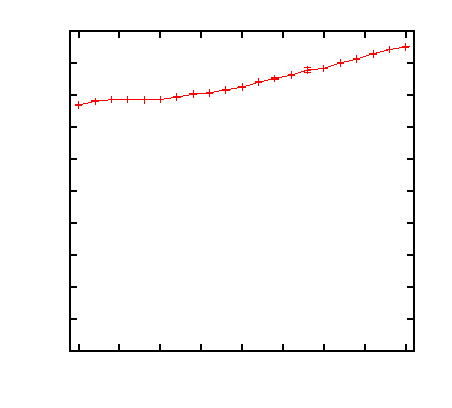
\includegraphics{CumulativeSumSkew_n8as16_Build_WallTime}}%
    \gplfronttext
  \end{picture}%
\endgroup

	\caption{Wall Time}
	\label{fig:CumulativeSumSkew_n8as16_Build_WallTime}
\end{subfigure}
\hfill
\begin{subfigure}{0.48\textwidth}
	% GNUPLOT: LaTeX picture with Postscript
\begingroup
  \makeatletter
  \providecommand\color[2][]{%
    \GenericError{(gnuplot) \space\space\space\@spaces}{%
      Package color not loaded in conjunction with
      terminal option `colourtext'%
    }{See the gnuplot documentation for explanation.%
    }{Either use 'blacktext' in gnuplot or load the package
      color.sty in LaTeX.}%
    \renewcommand\color[2][]{}%
  }%
  \providecommand\includegraphics[2][]{%
    \GenericError{(gnuplot) \space\space\space\@spaces}{%
      Package graphicx or graphics not loaded%
    }{See the gnuplot documentation for explanation.%
    }{The gnuplot epslatex terminal needs graphicx.sty or graphics.sty.}%
    \renewcommand\includegraphics[2][]{}%
  }%
  \providecommand\rotatebox[2]{#2}%
  \@ifundefined{ifGPcolor}{%
    \newif\ifGPcolor
    \GPcolortrue
  }{}%
  \@ifundefined{ifGPblacktext}{%
    \newif\ifGPblacktext
    \GPblacktexttrue
  }{}%
  % define a \g@addto@macro without @ in the name:
  \let\gplgaddtomacro\g@addto@macro
  % define empty templates for all commands taking text:
  \gdef\gplbacktext{}%
  \gdef\gplfronttext{}%
  \makeatother
  \ifGPblacktext
    % no textcolor at all
    \def\colorrgb#1{}%
    \def\colorgray#1{}%
  \else
    % gray or color?
    \ifGPcolor
      \def\colorrgb#1{\color[rgb]{#1}}%
      \def\colorgray#1{\color[gray]{#1}}%
      \expandafter\def\csname LTw\endcsname{\color{white}}%
      \expandafter\def\csname LTb\endcsname{\color{black}}%
      \expandafter\def\csname LTa\endcsname{\color{black}}%
      \expandafter\def\csname LT0\endcsname{\color[rgb]{1,0,0}}%
      \expandafter\def\csname LT1\endcsname{\color[rgb]{0,1,0}}%
      \expandafter\def\csname LT2\endcsname{\color[rgb]{0,0,1}}%
      \expandafter\def\csname LT3\endcsname{\color[rgb]{1,0,1}}%
      \expandafter\def\csname LT4\endcsname{\color[rgb]{0,1,1}}%
      \expandafter\def\csname LT5\endcsname{\color[rgb]{1,1,0}}%
      \expandafter\def\csname LT6\endcsname{\color[rgb]{0,0,0}}%
      \expandafter\def\csname LT7\endcsname{\color[rgb]{1,0.3,0}}%
      \expandafter\def\csname LT8\endcsname{\color[rgb]{0.5,0.5,0.5}}%
    \else
      % gray
      \def\colorrgb#1{\color{black}}%
      \def\colorgray#1{\color[gray]{#1}}%
      \expandafter\def\csname LTw\endcsname{\color{white}}%
      \expandafter\def\csname LTb\endcsname{\color{black}}%
      \expandafter\def\csname LTa\endcsname{\color{black}}%
      \expandafter\def\csname LT0\endcsname{\color{black}}%
      \expandafter\def\csname LT1\endcsname{\color{black}}%
      \expandafter\def\csname LT2\endcsname{\color{black}}%
      \expandafter\def\csname LT3\endcsname{\color{black}}%
      \expandafter\def\csname LT4\endcsname{\color{black}}%
      \expandafter\def\csname LT5\endcsname{\color{black}}%
      \expandafter\def\csname LT6\endcsname{\color{black}}%
      \expandafter\def\csname LT7\endcsname{\color{black}}%
      \expandafter\def\csname LT8\endcsname{\color{black}}%
    \fi
  \fi
  \setlength{\unitlength}{0.0500bp}%
  \begin{picture}(4030.00,3600.00)%
    \gplgaddtomacro\gplbacktext{%
      \csname LTb\endcsname%
      \put(516,384){\makebox(0,0)[r]{\strut{} 0}}%
      \put(516,725){\makebox(0,0)[r]{\strut{} 100}}%
      \put(516,1066){\makebox(0,0)[r]{\strut{} 200}}%
      \put(516,1408){\makebox(0,0)[r]{\strut{} 300}}%
      \put(516,1749){\makebox(0,0)[r]{\strut{} 400}}%
      \put(516,2090){\makebox(0,0)[r]{\strut{} 500}}%
      \put(516,2431){\makebox(0,0)[r]{\strut{} 600}}%
      \put(516,2773){\makebox(0,0)[r]{\strut{} 700}}%
      \put(516,3114){\makebox(0,0)[r]{\strut{} 800}}%
      \put(516,3455){\makebox(0,0)[r]{\strut{} 900}}%
      \put(665,264){\makebox(0,0){\strut{} 2}}%
      \put(1049,264){\makebox(0,0){\strut{} 2.5}}%
      \put(1433,264){\makebox(0,0){\strut{} 3}}%
      \put(1817,264){\makebox(0,0){\strut{} 3.5}}%
      \put(2201,264){\makebox(0,0){\strut{} 4}}%
      \put(2584,264){\makebox(0,0){\strut{} 4.5}}%
      \put(2968,264){\makebox(0,0){\strut{} 5}}%
      \put(3352,264){\makebox(0,0){\strut{} 5.5}}%
      \put(3736,264){\makebox(0,0){\strut{} 6}}%
      \put(96,1919){\rotatebox{-270}{\makebox(0,0){\strut{}Memory usage (MB)}}}%
      \put(2200,84){\makebox(0,0){\strut{}Blocksize (bits)}}%
    }%
    \gplgaddtomacro\gplfronttext{%
    }%
    \gplbacktext
    \put(0,0){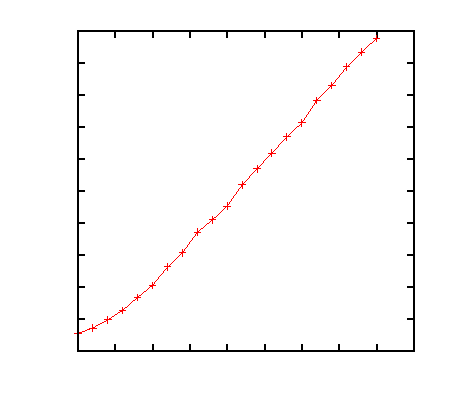
\includegraphics{CumulativeSumSkew_n8as16_build_memory}}%
    \gplfronttext
  \end{picture}%
\endgroup

	\caption{Memory Usage. Notice x-axis not starting at 0.}
	\label{fig:CumulativeSumSkew_n8as16_build_memory}
\end{subfigure}


\caption{Build Wall Time and Memory Usage of CumulativeSum for various skew.}
\label{fig:CumulativeSumSkew_n8as16_Build}
\end{figure}

\newgeometry{left=2cm,right=2cm, top=2cm, bottom=3cm}
\begin{figure}\tiny

\begin{subfigure}{0.48\textwidth}
	% GNUPLOT: LaTeX picture with Postscript
\begingroup
  \makeatletter
  \providecommand\color[2][]{%
    \GenericError{(gnuplot) \space\space\space\@spaces}{%
      Package color not loaded in conjunction with
      terminal option `colourtext'%
    }{See the gnuplot documentation for explanation.%
    }{Either use 'blacktext' in gnuplot or load the package
      color.sty in LaTeX.}%
    \renewcommand\color[2][]{}%
  }%
  \providecommand\includegraphics[2][]{%
    \GenericError{(gnuplot) \space\space\space\@spaces}{%
      Package graphicx or graphics not loaded%
    }{See the gnuplot documentation for explanation.%
    }{The gnuplot epslatex terminal needs graphicx.sty or graphics.sty.}%
    \renewcommand\includegraphics[2][]{}%
  }%
  \providecommand\rotatebox[2]{#2}%
  \@ifundefined{ifGPcolor}{%
    \newif\ifGPcolor
    \GPcolortrue
  }{}%
  \@ifundefined{ifGPblacktext}{%
    \newif\ifGPblacktext
    \GPblacktexttrue
  }{}%
  % define a \g@addto@macro without @ in the name:
  \let\gplgaddtomacro\g@addto@macro
  % define empty templates for all commands taking text:
  \gdef\gplbacktext{}%
  \gdef\gplfronttext{}%
  \makeatother
  \ifGPblacktext
    % no textcolor at all
    \def\colorrgb#1{}%
    \def\colorgray#1{}%
  \else
    % gray or color?
    \ifGPcolor
      \def\colorrgb#1{\color[rgb]{#1}}%
      \def\colorgray#1{\color[gray]{#1}}%
      \expandafter\def\csname LTw\endcsname{\color{white}}%
      \expandafter\def\csname LTb\endcsname{\color{black}}%
      \expandafter\def\csname LTa\endcsname{\color{black}}%
      \expandafter\def\csname LT0\endcsname{\color[rgb]{1,0,0}}%
      \expandafter\def\csname LT1\endcsname{\color[rgb]{0,1,0}}%
      \expandafter\def\csname LT2\endcsname{\color[rgb]{0,0,1}}%
      \expandafter\def\csname LT3\endcsname{\color[rgb]{1,0,1}}%
      \expandafter\def\csname LT4\endcsname{\color[rgb]{0,1,1}}%
      \expandafter\def\csname LT5\endcsname{\color[rgb]{1,1,0}}%
      \expandafter\def\csname LT6\endcsname{\color[rgb]{0,0,0}}%
      \expandafter\def\csname LT7\endcsname{\color[rgb]{1,0.3,0}}%
      \expandafter\def\csname LT8\endcsname{\color[rgb]{0.5,0.5,0.5}}%
    \else
      % gray
      \def\colorrgb#1{\color{black}}%
      \def\colorgray#1{\color[gray]{#1}}%
      \expandafter\def\csname LTw\endcsname{\color{white}}%
      \expandafter\def\csname LTb\endcsname{\color{black}}%
      \expandafter\def\csname LTa\endcsname{\color{black}}%
      \expandafter\def\csname LT0\endcsname{\color{black}}%
      \expandafter\def\csname LT1\endcsname{\color{black}}%
      \expandafter\def\csname LT2\endcsname{\color{black}}%
      \expandafter\def\csname LT3\endcsname{\color{black}}%
      \expandafter\def\csname LT4\endcsname{\color{black}}%
      \expandafter\def\csname LT5\endcsname{\color{black}}%
      \expandafter\def\csname LT6\endcsname{\color{black}}%
      \expandafter\def\csname LT7\endcsname{\color{black}}%
      \expandafter\def\csname LT8\endcsname{\color{black}}%
    \fi
  \fi
  \setlength{\unitlength}{0.0500bp}%
  \begin{picture}(4608.00,3600.00)%
    \gplgaddtomacro\gplbacktext{%
      \csname LTb\endcsname%
      \put(588,384){\makebox(0,0)[r]{\strut{} 0}}%
      \put(588,725){\makebox(0,0)[r]{\strut{} 200}}%
      \put(588,1066){\makebox(0,0)[r]{\strut{} 400}}%
      \put(588,1408){\makebox(0,0)[r]{\strut{} 600}}%
      \put(588,1749){\makebox(0,0)[r]{\strut{} 800}}%
      \put(588,2090){\makebox(0,0)[r]{\strut{} 1000}}%
      \put(588,2431){\makebox(0,0)[r]{\strut{} 1200}}%
      \put(588,2773){\makebox(0,0)[r]{\strut{} 1400}}%
      \put(588,3114){\makebox(0,0)[r]{\strut{} 1600}}%
      \put(588,3455){\makebox(0,0)[r]{\strut{} 1800}}%
      \put(749,264){\makebox(0,0){\strut{} 2}}%
      \put(1193,264){\makebox(0,0){\strut{} 2.5}}%
      \put(1637,264){\makebox(0,0){\strut{} 3}}%
      \put(2081,264){\makebox(0,0){\strut{} 3.5}}%
      \put(2526,264){\makebox(0,0){\strut{} 4}}%
      \put(2970,264){\makebox(0,0){\strut{} 4.5}}%
      \put(3414,264){\makebox(0,0){\strut{} 5}}%
      \put(3858,264){\makebox(0,0){\strut{} 5.5}}%
      \put(4302,264){\makebox(0,0){\strut{} 6}}%
      \put(96,1919){\rotatebox{-270}{\makebox(0,0){\strut{}Wall Time (seconds)}}}%
      \put(2525,84){\makebox(0,0){\strut{}Skew Parameter}}%
    }%
    \gplgaddtomacro\gplfronttext{%
    }%
    \gplbacktext
    \put(0,0){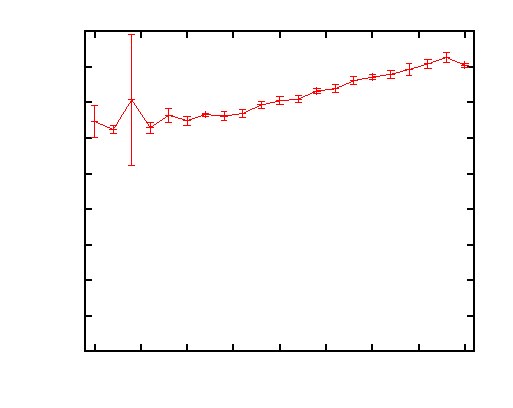
\includegraphics{CumulativeSumSkew_n8as16_Rank}}%
    \gplfronttext
  \end{picture}%
\endgroup

	\caption{Wall Time}
	\label{fig:CumulativeSumSkew_n8as16_Rank}
\end{subfigure}
\hfill
\begin{subfigure}{0.48\textwidth}
	% GNUPLOT: LaTeX picture with Postscript
\begingroup
  \makeatletter
  \providecommand\color[2][]{%
    \GenericError{(gnuplot) \space\space\space\@spaces}{%
      Package color not loaded in conjunction with
      terminal option `colourtext'%
    }{See the gnuplot documentation for explanation.%
    }{Either use 'blacktext' in gnuplot or load the package
      color.sty in LaTeX.}%
    \renewcommand\color[2][]{}%
  }%
  \providecommand\includegraphics[2][]{%
    \GenericError{(gnuplot) \space\space\space\@spaces}{%
      Package graphicx or graphics not loaded%
    }{See the gnuplot documentation for explanation.%
    }{The gnuplot epslatex terminal needs graphicx.sty or graphics.sty.}%
    \renewcommand\includegraphics[2][]{}%
  }%
  \providecommand\rotatebox[2]{#2}%
  \@ifundefined{ifGPcolor}{%
    \newif\ifGPcolor
    \GPcolortrue
  }{}%
  \@ifundefined{ifGPblacktext}{%
    \newif\ifGPblacktext
    \GPblacktexttrue
  }{}%
  % define a \g@addto@macro without @ in the name:
  \let\gplgaddtomacro\g@addto@macro
  % define empty templates for all commands taking text:
  \gdef\gplbacktext{}%
  \gdef\gplfronttext{}%
  \makeatother
  \ifGPblacktext
    % no textcolor at all
    \def\colorrgb#1{}%
    \def\colorgray#1{}%
  \else
    % gray or color?
    \ifGPcolor
      \def\colorrgb#1{\color[rgb]{#1}}%
      \def\colorgray#1{\color[gray]{#1}}%
      \expandafter\def\csname LTw\endcsname{\color{white}}%
      \expandafter\def\csname LTb\endcsname{\color{black}}%
      \expandafter\def\csname LTa\endcsname{\color{black}}%
      \expandafter\def\csname LT0\endcsname{\color[rgb]{1,0,0}}%
      \expandafter\def\csname LT1\endcsname{\color[rgb]{0,1,0}}%
      \expandafter\def\csname LT2\endcsname{\color[rgb]{0,0,1}}%
      \expandafter\def\csname LT3\endcsname{\color[rgb]{1,0,1}}%
      \expandafter\def\csname LT4\endcsname{\color[rgb]{0,1,1}}%
      \expandafter\def\csname LT5\endcsname{\color[rgb]{1,1,0}}%
      \expandafter\def\csname LT6\endcsname{\color[rgb]{0,0,0}}%
      \expandafter\def\csname LT7\endcsname{\color[rgb]{1,0.3,0}}%
      \expandafter\def\csname LT8\endcsname{\color[rgb]{0.5,0.5,0.5}}%
    \else
      % gray
      \def\colorrgb#1{\color{black}}%
      \def\colorgray#1{\color[gray]{#1}}%
      \expandafter\def\csname LTw\endcsname{\color{white}}%
      \expandafter\def\csname LTb\endcsname{\color{black}}%
      \expandafter\def\csname LTa\endcsname{\color{black}}%
      \expandafter\def\csname LT0\endcsname{\color{black}}%
      \expandafter\def\csname LT1\endcsname{\color{black}}%
      \expandafter\def\csname LT2\endcsname{\color{black}}%
      \expandafter\def\csname LT3\endcsname{\color{black}}%
      \expandafter\def\csname LT4\endcsname{\color{black}}%
      \expandafter\def\csname LT5\endcsname{\color{black}}%
      \expandafter\def\csname LT6\endcsname{\color{black}}%
      \expandafter\def\csname LT7\endcsname{\color{black}}%
      \expandafter\def\csname LT8\endcsname{\color{black}}%
    \fi
  \fi
  \setlength{\unitlength}{0.0500bp}%
  \begin{picture}(4608.00,3600.00)%
    \gplgaddtomacro\gplbacktext{%
      \csname LTb\endcsname%
      \put(660,384){\makebox(0,0)[r]{\strut{} 0}}%
      \put(660,823){\makebox(0,0)[r]{\strut{} 10000}}%
      \put(660,1261){\makebox(0,0)[r]{\strut{} 20000}}%
      \put(660,1700){\makebox(0,0)[r]{\strut{} 30000}}%
      \put(660,2139){\makebox(0,0)[r]{\strut{} 40000}}%
      \put(660,2578){\makebox(0,0)[r]{\strut{} 50000}}%
      \put(660,3016){\makebox(0,0)[r]{\strut{} 60000}}%
      \put(660,3455){\makebox(0,0)[r]{\strut{} 70000}}%
      \put(819,264){\makebox(0,0){\strut{} 2}}%
      \put(1255,264){\makebox(0,0){\strut{} 2.5}}%
      \put(1690,264){\makebox(0,0){\strut{} 3}}%
      \put(2126,264){\makebox(0,0){\strut{} 3.5}}%
      \put(2562,264){\makebox(0,0){\strut{} 4}}%
      \put(2997,264){\makebox(0,0){\strut{} 4.5}}%
      \put(3433,264){\makebox(0,0){\strut{} 5}}%
      \put(3868,264){\makebox(0,0){\strut{} 5.5}}%
      \put(4304,264){\makebox(0,0){\strut{} 6}}%
      \put(96,1919){\rotatebox{-270}{\makebox(0,0){\strut{}Cache Misses}}}%
      \put(2561,84){\makebox(0,0){\strut{}Skew Parameter}}%
    }%
    \gplgaddtomacro\gplfronttext{%
      \csname LTb\endcsname%
      \put(1308,3332){\makebox(0,0)[r]{\strut{}Level 1}}%
      \csname LTb\endcsname%
      \put(2307,3332){\makebox(0,0)[r]{\strut{}Level 2}}%
      \csname LTb\endcsname%
      \put(3306,3332){\makebox(0,0)[r]{\strut{}Level 3}}%
    }%
    \gplbacktext
    \put(0,0){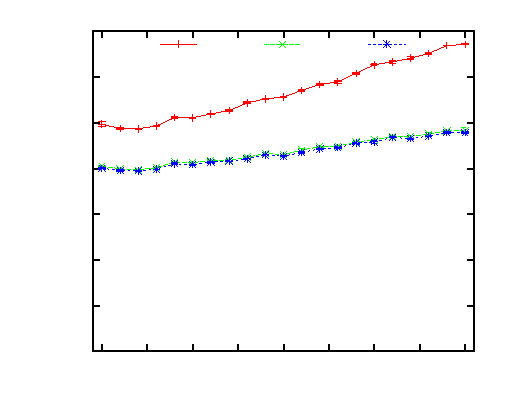
\includegraphics{CumulativeSumSkew_n8as16_Rank_CM}}%
    \gplfronttext
  \end{picture}%
\endgroup

	\caption{Cache Misses}
	\label{fig:CumulativeSumSkew_n8as16_Rank_CM}
\end{subfigure}

\begin{subfigure}{0.48\textwidth}
	% GNUPLOT: LaTeX picture with Postscript
\begingroup
  \makeatletter
  \providecommand\color[2][]{%
    \GenericError{(gnuplot) \space\space\space\@spaces}{%
      Package color not loaded in conjunction with
      terminal option `colourtext'%
    }{See the gnuplot documentation for explanation.%
    }{Either use 'blacktext' in gnuplot or load the package
      color.sty in LaTeX.}%
    \renewcommand\color[2][]{}%
  }%
  \providecommand\includegraphics[2][]{%
    \GenericError{(gnuplot) \space\space\space\@spaces}{%
      Package graphicx or graphics not loaded%
    }{See the gnuplot documentation for explanation.%
    }{The gnuplot epslatex terminal needs graphicx.sty or graphics.sty.}%
    \renewcommand\includegraphics[2][]{}%
  }%
  \providecommand\rotatebox[2]{#2}%
  \@ifundefined{ifGPcolor}{%
    \newif\ifGPcolor
    \GPcolortrue
  }{}%
  \@ifundefined{ifGPblacktext}{%
    \newif\ifGPblacktext
    \GPblacktexttrue
  }{}%
  % define a \g@addto@macro without @ in the name:
  \let\gplgaddtomacro\g@addto@macro
  % define empty templates for all commands taking text:
  \gdef\gplbacktext{}%
  \gdef\gplfronttext{}%
  \makeatother
  \ifGPblacktext
    % no textcolor at all
    \def\colorrgb#1{}%
    \def\colorgray#1{}%
  \else
    % gray or color?
    \ifGPcolor
      \def\colorrgb#1{\color[rgb]{#1}}%
      \def\colorgray#1{\color[gray]{#1}}%
      \expandafter\def\csname LTw\endcsname{\color{white}}%
      \expandafter\def\csname LTb\endcsname{\color{black}}%
      \expandafter\def\csname LTa\endcsname{\color{black}}%
      \expandafter\def\csname LT0\endcsname{\color[rgb]{1,0,0}}%
      \expandafter\def\csname LT1\endcsname{\color[rgb]{0,1,0}}%
      \expandafter\def\csname LT2\endcsname{\color[rgb]{0,0,1}}%
      \expandafter\def\csname LT3\endcsname{\color[rgb]{1,0,1}}%
      \expandafter\def\csname LT4\endcsname{\color[rgb]{0,1,1}}%
      \expandafter\def\csname LT5\endcsname{\color[rgb]{1,1,0}}%
      \expandafter\def\csname LT6\endcsname{\color[rgb]{0,0,0}}%
      \expandafter\def\csname LT7\endcsname{\color[rgb]{1,0.3,0}}%
      \expandafter\def\csname LT8\endcsname{\color[rgb]{0.5,0.5,0.5}}%
    \else
      % gray
      \def\colorrgb#1{\color{black}}%
      \def\colorgray#1{\color[gray]{#1}}%
      \expandafter\def\csname LTw\endcsname{\color{white}}%
      \expandafter\def\csname LTb\endcsname{\color{black}}%
      \expandafter\def\csname LTa\endcsname{\color{black}}%
      \expandafter\def\csname LT0\endcsname{\color{black}}%
      \expandafter\def\csname LT1\endcsname{\color{black}}%
      \expandafter\def\csname LT2\endcsname{\color{black}}%
      \expandafter\def\csname LT3\endcsname{\color{black}}%
      \expandafter\def\csname LT4\endcsname{\color{black}}%
      \expandafter\def\csname LT5\endcsname{\color{black}}%
      \expandafter\def\csname LT6\endcsname{\color{black}}%
      \expandafter\def\csname LT7\endcsname{\color{black}}%
      \expandafter\def\csname LT8\endcsname{\color{black}}%
    \fi
  \fi
  \setlength{\unitlength}{0.0500bp}%
  \begin{picture}(4608.00,3600.00)%
    \gplgaddtomacro\gplbacktext{%
      \csname LTb\endcsname%
      \put(660,384){\makebox(0,0)[r]{\strut{} 0}}%
      \put(660,1152){\makebox(0,0)[r]{\strut{} 5000}}%
      \put(660,1920){\makebox(0,0)[r]{\strut{} 10000}}%
      \put(660,2687){\makebox(0,0)[r]{\strut{} 15000}}%
      \put(660,3455){\makebox(0,0)[r]{\strut{} 20000}}%
      \put(806,264){\makebox(0,0){\strut{} 2}}%
      \put(1176,264){\makebox(0,0){\strut{} 2.5}}%
      \put(1546,264){\makebox(0,0){\strut{} 3}}%
      \put(1916,264){\makebox(0,0){\strut{} 3.5}}%
      \put(2286,264){\makebox(0,0){\strut{} 4}}%
      \put(2655,264){\makebox(0,0){\strut{} 4.5}}%
      \put(3025,264){\makebox(0,0){\strut{} 5}}%
      \put(3395,264){\makebox(0,0){\strut{} 5.5}}%
      \put(3765,264){\makebox(0,0){\strut{} 6}}%
      \put(3911,384){\makebox(0,0)[l]{\strut{} 0}}%
      \put(3911,998){\makebox(0,0)[l]{\strut{} 0.2}}%
      \put(3911,1612){\makebox(0,0)[l]{\strut{} 0.4}}%
      \put(3911,2227){\makebox(0,0)[l]{\strut{} 0.6}}%
      \put(3911,2841){\makebox(0,0)[l]{\strut{} 0.8}}%
      \put(3911,3455){\makebox(0,0)[l]{\strut{} 1}}%
      \put(96,1919){\rotatebox{-270}{\makebox(0,0){\strut{}Hits}}}%
      \put(4330,1919){\rotatebox{-270}{\makebox(0,0){\strut{}Hit Rate}}}%
      \put(2285,84){\makebox(0,0){\strut{}Skew Parameter}}%
    }%
    \gplgaddtomacro\gplfronttext{%
      \csname LTb\endcsname%
      \put(1380,3332){\makebox(0,0)[r]{\strut{}Hits}}%
      \csname LTb\endcsname%
      \put(2451,3332){\makebox(0,0)[r]{\strut{}Hit Rate}}%
    }%
    \gplbacktext
    \put(0,0){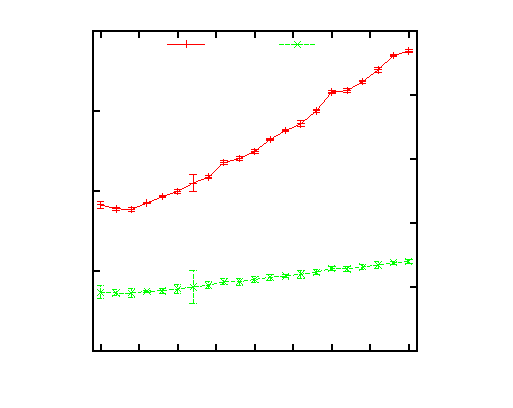
\includegraphics{CumulativeSumSkew_n8as16_Rank_L2CH}}%
    \gplfronttext
  \end{picture}%
\endgroup

	\caption{Level 2 Data Cache Hits \& Hit Rate}
	\label{fig:CumulativeSumSkew_n8as16_Rank_L2CH}
\end{subfigure}
\hfill
\begin{subfigure}{0.48\textwidth}
	% GNUPLOT: LaTeX picture with Postscript
\begingroup
  \makeatletter
  \providecommand\color[2][]{%
    \GenericError{(gnuplot) \space\space\space\@spaces}{%
      Package color not loaded in conjunction with
      terminal option `colourtext'%
    }{See the gnuplot documentation for explanation.%
    }{Either use 'blacktext' in gnuplot or load the package
      color.sty in LaTeX.}%
    \renewcommand\color[2][]{}%
  }%
  \providecommand\includegraphics[2][]{%
    \GenericError{(gnuplot) \space\space\space\@spaces}{%
      Package graphicx or graphics not loaded%
    }{See the gnuplot documentation for explanation.%
    }{The gnuplot epslatex terminal needs graphicx.sty or graphics.sty.}%
    \renewcommand\includegraphics[2][]{}%
  }%
  \providecommand\rotatebox[2]{#2}%
  \@ifundefined{ifGPcolor}{%
    \newif\ifGPcolor
    \GPcolortrue
  }{}%
  \@ifundefined{ifGPblacktext}{%
    \newif\ifGPblacktext
    \GPblacktexttrue
  }{}%
  % define a \g@addto@macro without @ in the name:
  \let\gplgaddtomacro\g@addto@macro
  % define empty templates for all commands taking text:
  \gdef\gplbacktext{}%
  \gdef\gplfronttext{}%
  \makeatother
  \ifGPblacktext
    % no textcolor at all
    \def\colorrgb#1{}%
    \def\colorgray#1{}%
  \else
    % gray or color?
    \ifGPcolor
      \def\colorrgb#1{\color[rgb]{#1}}%
      \def\colorgray#1{\color[gray]{#1}}%
      \expandafter\def\csname LTw\endcsname{\color{white}}%
      \expandafter\def\csname LTb\endcsname{\color{black}}%
      \expandafter\def\csname LTa\endcsname{\color{black}}%
      \expandafter\def\csname LT0\endcsname{\color[rgb]{1,0,0}}%
      \expandafter\def\csname LT1\endcsname{\color[rgb]{0,1,0}}%
      \expandafter\def\csname LT2\endcsname{\color[rgb]{0,0,1}}%
      \expandafter\def\csname LT3\endcsname{\color[rgb]{1,0,1}}%
      \expandafter\def\csname LT4\endcsname{\color[rgb]{0,1,1}}%
      \expandafter\def\csname LT5\endcsname{\color[rgb]{1,1,0}}%
      \expandafter\def\csname LT6\endcsname{\color[rgb]{0,0,0}}%
      \expandafter\def\csname LT7\endcsname{\color[rgb]{1,0.3,0}}%
      \expandafter\def\csname LT8\endcsname{\color[rgb]{0.5,0.5,0.5}}%
    \else
      % gray
      \def\colorrgb#1{\color{black}}%
      \def\colorgray#1{\color[gray]{#1}}%
      \expandafter\def\csname LTw\endcsname{\color{white}}%
      \expandafter\def\csname LTb\endcsname{\color{black}}%
      \expandafter\def\csname LTa\endcsname{\color{black}}%
      \expandafter\def\csname LT0\endcsname{\color{black}}%
      \expandafter\def\csname LT1\endcsname{\color{black}}%
      \expandafter\def\csname LT2\endcsname{\color{black}}%
      \expandafter\def\csname LT3\endcsname{\color{black}}%
      \expandafter\def\csname LT4\endcsname{\color{black}}%
      \expandafter\def\csname LT5\endcsname{\color{black}}%
      \expandafter\def\csname LT6\endcsname{\color{black}}%
      \expandafter\def\csname LT7\endcsname{\color{black}}%
      \expandafter\def\csname LT8\endcsname{\color{black}}%
    \fi
  \fi
  \setlength{\unitlength}{0.0500bp}%
  \begin{picture}(4608.00,3600.00)%
    \gplgaddtomacro\gplbacktext{%
      \csname LTb\endcsname%
      \put(732,384){\makebox(0,0)[r]{\strut{} 0}}%
      \put(732,896){\makebox(0,0)[r]{\strut{} 20000}}%
      \put(732,1408){\makebox(0,0)[r]{\strut{} 40000}}%
      \put(732,1920){\makebox(0,0)[r]{\strut{} 60000}}%
      \put(732,2431){\makebox(0,0)[r]{\strut{} 80000}}%
      \put(732,2943){\makebox(0,0)[r]{\strut{} 100000}}%
      \put(732,3455){\makebox(0,0)[r]{\strut{} 120000}}%
      \put(889,264){\makebox(0,0){\strut{} 2}}%
      \put(1316,264){\makebox(0,0){\strut{} 2.5}}%
      \put(1743,264){\makebox(0,0){\strut{} 3}}%
      \put(2170,264){\makebox(0,0){\strut{} 3.5}}%
      \put(2598,264){\makebox(0,0){\strut{} 4}}%
      \put(3025,264){\makebox(0,0){\strut{} 4.5}}%
      \put(3452,264){\makebox(0,0){\strut{} 5}}%
      \put(3879,264){\makebox(0,0){\strut{} 5.5}}%
      \put(4306,264){\makebox(0,0){\strut{} 6}}%
      \put(96,1919){\rotatebox{-270}{\makebox(0,0){\strut{}Branches Executed}}}%
      \put(2597,84){\makebox(0,0){\strut{}Skew Parameter}}%
    }%
    \gplgaddtomacro\gplfronttext{%
    }%
    \gplbacktext
    \put(0,0){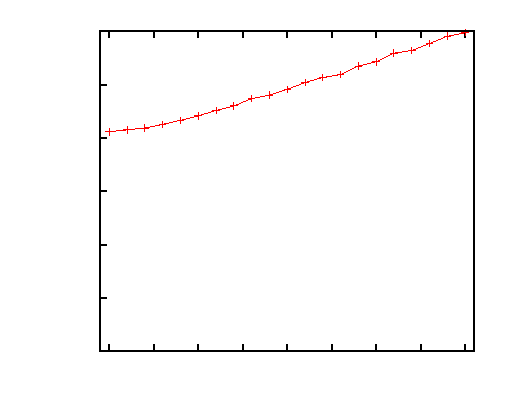
\includegraphics{CumulativeSumSkew_n8as16_Rank_BMExe}}%
    \gplfronttext
  \end{picture}%
\endgroup

	\caption{Branches Executed}
	\label{fig:CumulativeSumSkew_n8as16_Rank_BMExe}
\end{subfigure}

\begin{subfigure}{0.48\textwidth}
	% GNUPLOT: LaTeX picture with Postscript
\begingroup
  \makeatletter
  \providecommand\color[2][]{%
    \GenericError{(gnuplot) \space\space\space\@spaces}{%
      Package color not loaded in conjunction with
      terminal option `colourtext'%
    }{See the gnuplot documentation for explanation.%
    }{Either use 'blacktext' in gnuplot or load the package
      color.sty in LaTeX.}%
    \renewcommand\color[2][]{}%
  }%
  \providecommand\includegraphics[2][]{%
    \GenericError{(gnuplot) \space\space\space\@spaces}{%
      Package graphicx or graphics not loaded%
    }{See the gnuplot documentation for explanation.%
    }{The gnuplot epslatex terminal needs graphicx.sty or graphics.sty.}%
    \renewcommand\includegraphics[2][]{}%
  }%
  \providecommand\rotatebox[2]{#2}%
  \@ifundefined{ifGPcolor}{%
    \newif\ifGPcolor
    \GPcolortrue
  }{}%
  \@ifundefined{ifGPblacktext}{%
    \newif\ifGPblacktext
    \GPblacktexttrue
  }{}%
  % define a \g@addto@macro without @ in the name:
  \let\gplgaddtomacro\g@addto@macro
  % define empty templates for all commands taking text:
  \gdef\gplbacktext{}%
  \gdef\gplfronttext{}%
  \makeatother
  \ifGPblacktext
    % no textcolor at all
    \def\colorrgb#1{}%
    \def\colorgray#1{}%
  \else
    % gray or color?
    \ifGPcolor
      \def\colorrgb#1{\color[rgb]{#1}}%
      \def\colorgray#1{\color[gray]{#1}}%
      \expandafter\def\csname LTw\endcsname{\color{white}}%
      \expandafter\def\csname LTb\endcsname{\color{black}}%
      \expandafter\def\csname LTa\endcsname{\color{black}}%
      \expandafter\def\csname LT0\endcsname{\color[rgb]{1,0,0}}%
      \expandafter\def\csname LT1\endcsname{\color[rgb]{0,1,0}}%
      \expandafter\def\csname LT2\endcsname{\color[rgb]{0,0,1}}%
      \expandafter\def\csname LT3\endcsname{\color[rgb]{1,0,1}}%
      \expandafter\def\csname LT4\endcsname{\color[rgb]{0,1,1}}%
      \expandafter\def\csname LT5\endcsname{\color[rgb]{1,1,0}}%
      \expandafter\def\csname LT6\endcsname{\color[rgb]{0,0,0}}%
      \expandafter\def\csname LT7\endcsname{\color[rgb]{1,0.3,0}}%
      \expandafter\def\csname LT8\endcsname{\color[rgb]{0.5,0.5,0.5}}%
    \else
      % gray
      \def\colorrgb#1{\color{black}}%
      \def\colorgray#1{\color[gray]{#1}}%
      \expandafter\def\csname LTw\endcsname{\color{white}}%
      \expandafter\def\csname LTb\endcsname{\color{black}}%
      \expandafter\def\csname LTa\endcsname{\color{black}}%
      \expandafter\def\csname LT0\endcsname{\color{black}}%
      \expandafter\def\csname LT1\endcsname{\color{black}}%
      \expandafter\def\csname LT2\endcsname{\color{black}}%
      \expandafter\def\csname LT3\endcsname{\color{black}}%
      \expandafter\def\csname LT4\endcsname{\color{black}}%
      \expandafter\def\csname LT5\endcsname{\color{black}}%
      \expandafter\def\csname LT6\endcsname{\color{black}}%
      \expandafter\def\csname LT7\endcsname{\color{black}}%
      \expandafter\def\csname LT8\endcsname{\color{black}}%
    \fi
  \fi
  \setlength{\unitlength}{0.0500bp}%
  \begin{picture}(4608.00,3600.00)%
    \gplgaddtomacro\gplbacktext{%
      \csname LTb\endcsname%
      \put(660,384){\makebox(0,0)[r]{\strut{} 0}}%
      \put(660,998){\makebox(0,0)[r]{\strut{} 2000}}%
      \put(660,1612){\makebox(0,0)[r]{\strut{} 4000}}%
      \put(660,2227){\makebox(0,0)[r]{\strut{} 6000}}%
      \put(660,2841){\makebox(0,0)[r]{\strut{} 8000}}%
      \put(660,3455){\makebox(0,0)[r]{\strut{} 10000}}%
      \put(806,264){\makebox(0,0){\strut{} 2}}%
      \put(1176,264){\makebox(0,0){\strut{} 2.5}}%
      \put(1546,264){\makebox(0,0){\strut{} 3}}%
      \put(1916,264){\makebox(0,0){\strut{} 3.5}}%
      \put(2286,264){\makebox(0,0){\strut{} 4}}%
      \put(2655,264){\makebox(0,0){\strut{} 4.5}}%
      \put(3025,264){\makebox(0,0){\strut{} 5}}%
      \put(3395,264){\makebox(0,0){\strut{} 5.5}}%
      \put(3765,264){\makebox(0,0){\strut{} 6}}%
      \put(3911,384){\makebox(0,0)[l]{\strut{} 0}}%
      \put(3911,998){\makebox(0,0)[l]{\strut{} 0.2}}%
      \put(3911,1612){\makebox(0,0)[l]{\strut{} 0.4}}%
      \put(3911,2227){\makebox(0,0)[l]{\strut{} 0.6}}%
      \put(3911,2841){\makebox(0,0)[l]{\strut{} 0.8}}%
      \put(3911,3455){\makebox(0,0)[l]{\strut{} 1}}%
      \put(96,1919){\rotatebox{-270}{\makebox(0,0){\strut{}Branch Mispredictions}}}%
      \put(4330,1919){\rotatebox{-270}{\makebox(0,0){\strut{}Branch Misprediction Rate}}}%
      \put(2285,84){\makebox(0,0){\strut{}Skew Parameter}}%
    }%
    \gplgaddtomacro\gplfronttext{%
      \csname LTb\endcsname%
      \put(2604,3332){\makebox(0,0)[r]{\strut{}Branch Mispredictions}}%
      \csname LTb\endcsname%
      \put(2604,3212){\makebox(0,0)[r]{\strut{}Branch Misprediction Rate}}%
    }%
    \gplbacktext
    \put(0,0){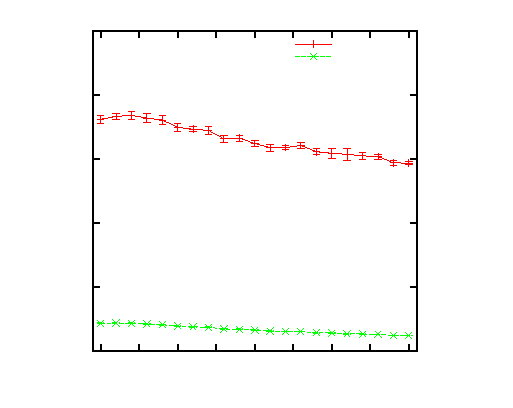
\includegraphics{CumulativeSumSkew_n8as16_Rank_BM}}%
    \gplfronttext
  \end{picture}%
\endgroup

	\caption{Branch Mispredictions}
	\label{fig:CumulativeSumSkew_n8as16_Rank_BM}
\end{subfigure}
\hfill
\begin{subfigure}{0.48\textwidth}
	% GNUPLOT: LaTeX picture with Postscript
\begingroup
  \makeatletter
  \providecommand\color[2][]{%
    \GenericError{(gnuplot) \space\space\space\@spaces}{%
      Package color not loaded in conjunction with
      terminal option `colourtext'%
    }{See the gnuplot documentation for explanation.%
    }{Either use 'blacktext' in gnuplot or load the package
      color.sty in LaTeX.}%
    \renewcommand\color[2][]{}%
  }%
  \providecommand\includegraphics[2][]{%
    \GenericError{(gnuplot) \space\space\space\@spaces}{%
      Package graphicx or graphics not loaded%
    }{See the gnuplot documentation for explanation.%
    }{The gnuplot epslatex terminal needs graphicx.sty or graphics.sty.}%
    \renewcommand\includegraphics[2][]{}%
  }%
  \providecommand\rotatebox[2]{#2}%
  \@ifundefined{ifGPcolor}{%
    \newif\ifGPcolor
    \GPcolortrue
  }{}%
  \@ifundefined{ifGPblacktext}{%
    \newif\ifGPblacktext
    \GPblacktexttrue
  }{}%
  % define a \g@addto@macro without @ in the name:
  \let\gplgaddtomacro\g@addto@macro
  % define empty templates for all commands taking text:
  \gdef\gplbacktext{}%
  \gdef\gplfronttext{}%
  \makeatother
  \ifGPblacktext
    % no textcolor at all
    \def\colorrgb#1{}%
    \def\colorgray#1{}%
  \else
    % gray or color?
    \ifGPcolor
      \def\colorrgb#1{\color[rgb]{#1}}%
      \def\colorgray#1{\color[gray]{#1}}%
      \expandafter\def\csname LTw\endcsname{\color{white}}%
      \expandafter\def\csname LTb\endcsname{\color{black}}%
      \expandafter\def\csname LTa\endcsname{\color{black}}%
      \expandafter\def\csname LT0\endcsname{\color[rgb]{1,0,0}}%
      \expandafter\def\csname LT1\endcsname{\color[rgb]{0,1,0}}%
      \expandafter\def\csname LT2\endcsname{\color[rgb]{0,0,1}}%
      \expandafter\def\csname LT3\endcsname{\color[rgb]{1,0,1}}%
      \expandafter\def\csname LT4\endcsname{\color[rgb]{0,1,1}}%
      \expandafter\def\csname LT5\endcsname{\color[rgb]{1,1,0}}%
      \expandafter\def\csname LT6\endcsname{\color[rgb]{0,0,0}}%
      \expandafter\def\csname LT7\endcsname{\color[rgb]{1,0.3,0}}%
      \expandafter\def\csname LT8\endcsname{\color[rgb]{0.5,0.5,0.5}}%
    \else
      % gray
      \def\colorrgb#1{\color{black}}%
      \def\colorgray#1{\color[gray]{#1}}%
      \expandafter\def\csname LTw\endcsname{\color{white}}%
      \expandafter\def\csname LTb\endcsname{\color{black}}%
      \expandafter\def\csname LTa\endcsname{\color{black}}%
      \expandafter\def\csname LT0\endcsname{\color{black}}%
      \expandafter\def\csname LT1\endcsname{\color{black}}%
      \expandafter\def\csname LT2\endcsname{\color{black}}%
      \expandafter\def\csname LT3\endcsname{\color{black}}%
      \expandafter\def\csname LT4\endcsname{\color{black}}%
      \expandafter\def\csname LT5\endcsname{\color{black}}%
      \expandafter\def\csname LT6\endcsname{\color{black}}%
      \expandafter\def\csname LT7\endcsname{\color{black}}%
      \expandafter\def\csname LT8\endcsname{\color{black}}%
    \fi
  \fi
  \setlength{\unitlength}{0.0500bp}%
  \begin{picture}(4608.00,3600.00)%
    \gplgaddtomacro\gplbacktext{%
      \csname LTb\endcsname%
      \put(660,384){\makebox(0,0)[r]{\strut{} 0}}%
      \put(660,896){\makebox(0,0)[r]{\strut{} 2000}}%
      \put(660,1408){\makebox(0,0)[r]{\strut{} 4000}}%
      \put(660,1920){\makebox(0,0)[r]{\strut{} 6000}}%
      \put(660,2431){\makebox(0,0)[r]{\strut{} 8000}}%
      \put(660,2943){\makebox(0,0)[r]{\strut{} 10000}}%
      \put(660,3455){\makebox(0,0)[r]{\strut{} 12000}}%
      \put(819,264){\makebox(0,0){\strut{} 2}}%
      \put(1255,264){\makebox(0,0){\strut{} 2.5}}%
      \put(1690,264){\makebox(0,0){\strut{} 3}}%
      \put(2126,264){\makebox(0,0){\strut{} 3.5}}%
      \put(2562,264){\makebox(0,0){\strut{} 4}}%
      \put(2997,264){\makebox(0,0){\strut{} 4.5}}%
      \put(3433,264){\makebox(0,0){\strut{} 5}}%
      \put(3868,264){\makebox(0,0){\strut{} 5.5}}%
      \put(4304,264){\makebox(0,0){\strut{} 6}}%
      \put(96,1919){\rotatebox{-270}{\makebox(0,0){\strut{}Translation Lookaside Buffer Misses}}}%
      \put(2561,84){\makebox(0,0){\strut{}Skew Parameter}}%
    }%
    \gplgaddtomacro\gplfronttext{%
    }%
    \gplbacktext
    \put(0,0){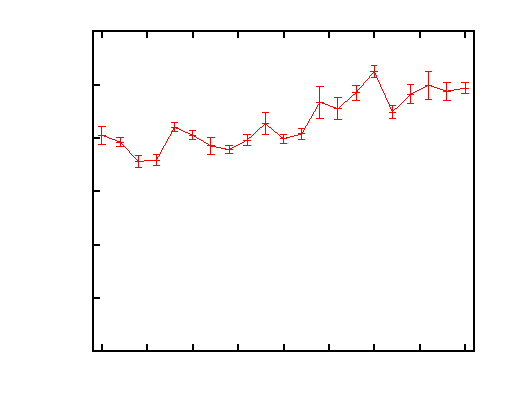
\includegraphics{CumulativeSumSkew_n8as16_Rank_TLBM}}%
    \gplfronttext
  \end{picture}%
\endgroup

	\caption{Translation Lookaside Buffer Misses}
	\label{fig:CumulativeSumSkew_n8as16_Rank_TLBM}
\end{subfigure}

\caption{Measurements for Rank Queries on CumulativeSum for various skew.}
\label{fig:CumulativeSumSkew_n8as16_Rank}
\end{figure}






\begin{figure}\tiny

\begin{subfigure}{0.48\textwidth}
	% GNUPLOT: LaTeX picture with Postscript
\begingroup
  \makeatletter
  \providecommand\color[2][]{%
    \GenericError{(gnuplot) \space\space\space\@spaces}{%
      Package color not loaded in conjunction with
      terminal option `colourtext'%
    }{See the gnuplot documentation for explanation.%
    }{Either use 'blacktext' in gnuplot or load the package
      color.sty in LaTeX.}%
    \renewcommand\color[2][]{}%
  }%
  \providecommand\includegraphics[2][]{%
    \GenericError{(gnuplot) \space\space\space\@spaces}{%
      Package graphicx or graphics not loaded%
    }{See the gnuplot documentation for explanation.%
    }{The gnuplot epslatex terminal needs graphicx.sty or graphics.sty.}%
    \renewcommand\includegraphics[2][]{}%
  }%
  \providecommand\rotatebox[2]{#2}%
  \@ifundefined{ifGPcolor}{%
    \newif\ifGPcolor
    \GPcolortrue
  }{}%
  \@ifundefined{ifGPblacktext}{%
    \newif\ifGPblacktext
    \GPblacktexttrue
  }{}%
  % define a \g@addto@macro without @ in the name:
  \let\gplgaddtomacro\g@addto@macro
  % define empty templates for all commands taking text:
  \gdef\gplbacktext{}%
  \gdef\gplfronttext{}%
  \makeatother
  \ifGPblacktext
    % no textcolor at all
    \def\colorrgb#1{}%
    \def\colorgray#1{}%
  \else
    % gray or color?
    \ifGPcolor
      \def\colorrgb#1{\color[rgb]{#1}}%
      \def\colorgray#1{\color[gray]{#1}}%
      \expandafter\def\csname LTw\endcsname{\color{white}}%
      \expandafter\def\csname LTb\endcsname{\color{black}}%
      \expandafter\def\csname LTa\endcsname{\color{black}}%
      \expandafter\def\csname LT0\endcsname{\color[rgb]{1,0,0}}%
      \expandafter\def\csname LT1\endcsname{\color[rgb]{0,1,0}}%
      \expandafter\def\csname LT2\endcsname{\color[rgb]{0,0,1}}%
      \expandafter\def\csname LT3\endcsname{\color[rgb]{1,0,1}}%
      \expandafter\def\csname LT4\endcsname{\color[rgb]{0,1,1}}%
      \expandafter\def\csname LT5\endcsname{\color[rgb]{1,1,0}}%
      \expandafter\def\csname LT6\endcsname{\color[rgb]{0,0,0}}%
      \expandafter\def\csname LT7\endcsname{\color[rgb]{1,0.3,0}}%
      \expandafter\def\csname LT8\endcsname{\color[rgb]{0.5,0.5,0.5}}%
    \else
      % gray
      \def\colorrgb#1{\color{black}}%
      \def\colorgray#1{\color[gray]{#1}}%
      \expandafter\def\csname LTw\endcsname{\color{white}}%
      \expandafter\def\csname LTb\endcsname{\color{black}}%
      \expandafter\def\csname LTa\endcsname{\color{black}}%
      \expandafter\def\csname LT0\endcsname{\color{black}}%
      \expandafter\def\csname LT1\endcsname{\color{black}}%
      \expandafter\def\csname LT2\endcsname{\color{black}}%
      \expandafter\def\csname LT3\endcsname{\color{black}}%
      \expandafter\def\csname LT4\endcsname{\color{black}}%
      \expandafter\def\csname LT5\endcsname{\color{black}}%
      \expandafter\def\csname LT6\endcsname{\color{black}}%
      \expandafter\def\csname LT7\endcsname{\color{black}}%
      \expandafter\def\csname LT8\endcsname{\color{black}}%
    \fi
  \fi
  \setlength{\unitlength}{0.0500bp}%
  \begin{picture}(4608.00,3600.00)%
    \gplgaddtomacro\gplbacktext{%
      \csname LTb\endcsname%
      \put(588,384){\makebox(0,0)[r]{\strut{} 0}}%
      \put(588,725){\makebox(0,0)[r]{\strut{} 1000}}%
      \put(588,1066){\makebox(0,0)[r]{\strut{} 2000}}%
      \put(588,1408){\makebox(0,0)[r]{\strut{} 3000}}%
      \put(588,1749){\makebox(0,0)[r]{\strut{} 4000}}%
      \put(588,2090){\makebox(0,0)[r]{\strut{} 5000}}%
      \put(588,2431){\makebox(0,0)[r]{\strut{} 6000}}%
      \put(588,2773){\makebox(0,0)[r]{\strut{} 7000}}%
      \put(588,3114){\makebox(0,0)[r]{\strut{} 8000}}%
      \put(588,3455){\makebox(0,0)[r]{\strut{} 9000}}%
      \put(749,264){\makebox(0,0){\strut{} 2}}%
      \put(1193,264){\makebox(0,0){\strut{} 2.5}}%
      \put(1637,264){\makebox(0,0){\strut{} 3}}%
      \put(2081,264){\makebox(0,0){\strut{} 3.5}}%
      \put(2526,264){\makebox(0,0){\strut{} 4}}%
      \put(2970,264){\makebox(0,0){\strut{} 4.5}}%
      \put(3414,264){\makebox(0,0){\strut{} 5}}%
      \put(3858,264){\makebox(0,0){\strut{} 5.5}}%
      \put(4302,264){\makebox(0,0){\strut{} 6}}%
      \put(96,1919){\rotatebox{-270}{\makebox(0,0){\strut{}Wall Time ($\mu s$)}}}%
      \put(2525,84){\makebox(0,0){\strut{}Skew Parameter}}%
    }%
    \gplgaddtomacro\gplfronttext{%
      \csname LTb\endcsname%
      \put(1668,3332){\makebox(0,0)[r]{\strut{}CumulativeSum}}%
    }%
    \gplbacktext
    \put(0,0){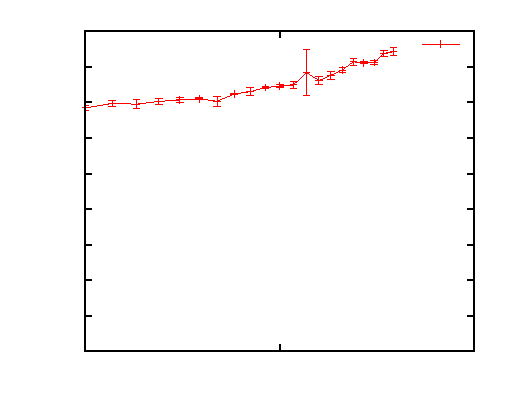
\includegraphics{CumulativeSumSkew_n8as16_Select}}%
    \gplfronttext
  \end{picture}%
\endgroup

	\caption{Wall Time}
	\label{fig:CumulativeSumSkew_n8as16_Select}
\end{subfigure}
\hfill
\begin{subfigure}{0.48\textwidth}
	% GNUPLOT: LaTeX picture with Postscript
\begingroup
  \makeatletter
  \providecommand\color[2][]{%
    \GenericError{(gnuplot) \space\space\space\@spaces}{%
      Package color not loaded in conjunction with
      terminal option `colourtext'%
    }{See the gnuplot documentation for explanation.%
    }{Either use 'blacktext' in gnuplot or load the package
      color.sty in LaTeX.}%
    \renewcommand\color[2][]{}%
  }%
  \providecommand\includegraphics[2][]{%
    \GenericError{(gnuplot) \space\space\space\@spaces}{%
      Package graphicx or graphics not loaded%
    }{See the gnuplot documentation for explanation.%
    }{The gnuplot epslatex terminal needs graphicx.sty or graphics.sty.}%
    \renewcommand\includegraphics[2][]{}%
  }%
  \providecommand\rotatebox[2]{#2}%
  \@ifundefined{ifGPcolor}{%
    \newif\ifGPcolor
    \GPcolortrue
  }{}%
  \@ifundefined{ifGPblacktext}{%
    \newif\ifGPblacktext
    \GPblacktexttrue
  }{}%
  % define a \g@addto@macro without @ in the name:
  \let\gplgaddtomacro\g@addto@macro
  % define empty templates for all commands taking text:
  \gdef\gplbacktext{}%
  \gdef\gplfronttext{}%
  \makeatother
  \ifGPblacktext
    % no textcolor at all
    \def\colorrgb#1{}%
    \def\colorgray#1{}%
  \else
    % gray or color?
    \ifGPcolor
      \def\colorrgb#1{\color[rgb]{#1}}%
      \def\colorgray#1{\color[gray]{#1}}%
      \expandafter\def\csname LTw\endcsname{\color{white}}%
      \expandafter\def\csname LTb\endcsname{\color{black}}%
      \expandafter\def\csname LTa\endcsname{\color{black}}%
      \expandafter\def\csname LT0\endcsname{\color[rgb]{1,0,0}}%
      \expandafter\def\csname LT1\endcsname{\color[rgb]{0,1,0}}%
      \expandafter\def\csname LT2\endcsname{\color[rgb]{0,0,1}}%
      \expandafter\def\csname LT3\endcsname{\color[rgb]{1,0,1}}%
      \expandafter\def\csname LT4\endcsname{\color[rgb]{0,1,1}}%
      \expandafter\def\csname LT5\endcsname{\color[rgb]{1,1,0}}%
      \expandafter\def\csname LT6\endcsname{\color[rgb]{0,0,0}}%
      \expandafter\def\csname LT7\endcsname{\color[rgb]{1,0.3,0}}%
      \expandafter\def\csname LT8\endcsname{\color[rgb]{0.5,0.5,0.5}}%
    \else
      % gray
      \def\colorrgb#1{\color{black}}%
      \def\colorgray#1{\color[gray]{#1}}%
      \expandafter\def\csname LTw\endcsname{\color{white}}%
      \expandafter\def\csname LTb\endcsname{\color{black}}%
      \expandafter\def\csname LTa\endcsname{\color{black}}%
      \expandafter\def\csname LT0\endcsname{\color{black}}%
      \expandafter\def\csname LT1\endcsname{\color{black}}%
      \expandafter\def\csname LT2\endcsname{\color{black}}%
      \expandafter\def\csname LT3\endcsname{\color{black}}%
      \expandafter\def\csname LT4\endcsname{\color{black}}%
      \expandafter\def\csname LT5\endcsname{\color{black}}%
      \expandafter\def\csname LT6\endcsname{\color{black}}%
      \expandafter\def\csname LT7\endcsname{\color{black}}%
      \expandafter\def\csname LT8\endcsname{\color{black}}%
    \fi
  \fi
  \setlength{\unitlength}{0.0500bp}%
  \begin{picture}(4608.00,3600.00)%
    \gplgaddtomacro\gplbacktext{%
      \csname LTb\endcsname%
      \put(732,384){\makebox(0,0)[r]{\strut{} 0}}%
      \put(732,768){\makebox(0,0)[r]{\strut{} 50000}}%
      \put(732,1152){\makebox(0,0)[r]{\strut{} 100000}}%
      \put(732,1536){\makebox(0,0)[r]{\strut{} 150000}}%
      \put(732,1920){\makebox(0,0)[r]{\strut{} 200000}}%
      \put(732,2303){\makebox(0,0)[r]{\strut{} 250000}}%
      \put(732,2687){\makebox(0,0)[r]{\strut{} 300000}}%
      \put(732,3071){\makebox(0,0)[r]{\strut{} 350000}}%
      \put(732,3455){\makebox(0,0)[r]{\strut{} 400000}}%
      \put(889,264){\makebox(0,0){\strut{} 2}}%
      \put(1316,264){\makebox(0,0){\strut{} 2.5}}%
      \put(1743,264){\makebox(0,0){\strut{} 3}}%
      \put(2170,264){\makebox(0,0){\strut{} 3.5}}%
      \put(2598,264){\makebox(0,0){\strut{} 4}}%
      \put(3025,264){\makebox(0,0){\strut{} 4.5}}%
      \put(3452,264){\makebox(0,0){\strut{} 5}}%
      \put(3879,264){\makebox(0,0){\strut{} 5.5}}%
      \put(4306,264){\makebox(0,0){\strut{} 6}}%
      \put(96,1919){\rotatebox{-270}{\makebox(0,0){\strut{}Cache Misses}}}%
      \put(2597,84){\makebox(0,0){\strut{}Skew Parameter}}%
    }%
    \gplgaddtomacro\gplfronttext{%
      \csname LTb\endcsname%
      \put(1380,3332){\makebox(0,0)[r]{\strut{}Level 1}}%
      \csname LTb\endcsname%
      \put(2379,3332){\makebox(0,0)[r]{\strut{}Level 2}}%
      \csname LTb\endcsname%
      \put(3378,3332){\makebox(0,0)[r]{\strut{}Level 3}}%
    }%
    \gplbacktext
    \put(0,0){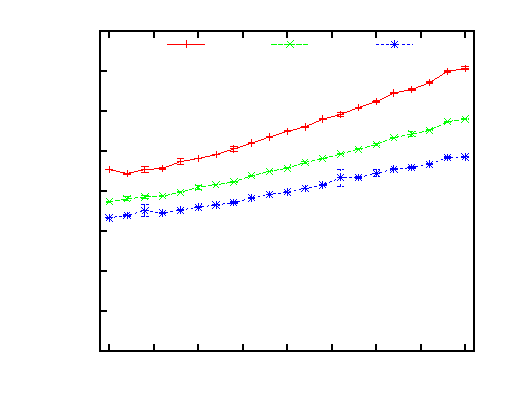
\includegraphics{CumulativeSumSkew_n8as16_Select_CM}}%
    \gplfronttext
  \end{picture}%
\endgroup

	\caption{Cache Misses}
	\label{fig:CumulativeSumSkew_n8as16_Select_CM}
\end{subfigure}

\begin{subfigure}{0.48\textwidth}
	% GNUPLOT: LaTeX picture with Postscript
\begingroup
  \makeatletter
  \providecommand\color[2][]{%
    \GenericError{(gnuplot) \space\space\space\@spaces}{%
      Package color not loaded in conjunction with
      terminal option `colourtext'%
    }{See the gnuplot documentation for explanation.%
    }{Either use 'blacktext' in gnuplot or load the package
      color.sty in LaTeX.}%
    \renewcommand\color[2][]{}%
  }%
  \providecommand\includegraphics[2][]{%
    \GenericError{(gnuplot) \space\space\space\@spaces}{%
      Package graphicx or graphics not loaded%
    }{See the gnuplot documentation for explanation.%
    }{The gnuplot epslatex terminal needs graphicx.sty or graphics.sty.}%
    \renewcommand\includegraphics[2][]{}%
  }%
  \providecommand\rotatebox[2]{#2}%
  \@ifundefined{ifGPcolor}{%
    \newif\ifGPcolor
    \GPcolortrue
  }{}%
  \@ifundefined{ifGPblacktext}{%
    \newif\ifGPblacktext
    \GPblacktexttrue
  }{}%
  % define a \g@addto@macro without @ in the name:
  \let\gplgaddtomacro\g@addto@macro
  % define empty templates for all commands taking text:
  \gdef\gplbacktext{}%
  \gdef\gplfronttext{}%
  \makeatother
  \ifGPblacktext
    % no textcolor at all
    \def\colorrgb#1{}%
    \def\colorgray#1{}%
  \else
    % gray or color?
    \ifGPcolor
      \def\colorrgb#1{\color[rgb]{#1}}%
      \def\colorgray#1{\color[gray]{#1}}%
      \expandafter\def\csname LTw\endcsname{\color{white}}%
      \expandafter\def\csname LTb\endcsname{\color{black}}%
      \expandafter\def\csname LTa\endcsname{\color{black}}%
      \expandafter\def\csname LT0\endcsname{\color[rgb]{1,0,0}}%
      \expandafter\def\csname LT1\endcsname{\color[rgb]{0,1,0}}%
      \expandafter\def\csname LT2\endcsname{\color[rgb]{0,0,1}}%
      \expandafter\def\csname LT3\endcsname{\color[rgb]{1,0,1}}%
      \expandafter\def\csname LT4\endcsname{\color[rgb]{0,1,1}}%
      \expandafter\def\csname LT5\endcsname{\color[rgb]{1,1,0}}%
      \expandafter\def\csname LT6\endcsname{\color[rgb]{0,0,0}}%
      \expandafter\def\csname LT7\endcsname{\color[rgb]{1,0.3,0}}%
      \expandafter\def\csname LT8\endcsname{\color[rgb]{0.5,0.5,0.5}}%
    \else
      % gray
      \def\colorrgb#1{\color{black}}%
      \def\colorgray#1{\color[gray]{#1}}%
      \expandafter\def\csname LTw\endcsname{\color{white}}%
      \expandafter\def\csname LTb\endcsname{\color{black}}%
      \expandafter\def\csname LTa\endcsname{\color{black}}%
      \expandafter\def\csname LT0\endcsname{\color{black}}%
      \expandafter\def\csname LT1\endcsname{\color{black}}%
      \expandafter\def\csname LT2\endcsname{\color{black}}%
      \expandafter\def\csname LT3\endcsname{\color{black}}%
      \expandafter\def\csname LT4\endcsname{\color{black}}%
      \expandafter\def\csname LT5\endcsname{\color{black}}%
      \expandafter\def\csname LT6\endcsname{\color{black}}%
      \expandafter\def\csname LT7\endcsname{\color{black}}%
      \expandafter\def\csname LT8\endcsname{\color{black}}%
    \fi
  \fi
  \setlength{\unitlength}{0.0500bp}%
  \begin{picture}(4608.00,3600.00)%
    \gplgaddtomacro\gplbacktext{%
      \csname LTb\endcsname%
      \put(660,384){\makebox(0,0)[r]{\strut{} 0}}%
      \put(660,823){\makebox(0,0)[r]{\strut{} 10000}}%
      \put(660,1261){\makebox(0,0)[r]{\strut{} 20000}}%
      \put(660,1700){\makebox(0,0)[r]{\strut{} 30000}}%
      \put(660,2139){\makebox(0,0)[r]{\strut{} 40000}}%
      \put(660,2578){\makebox(0,0)[r]{\strut{} 50000}}%
      \put(660,3016){\makebox(0,0)[r]{\strut{} 60000}}%
      \put(660,3455){\makebox(0,0)[r]{\strut{} 70000}}%
      \put(806,264){\makebox(0,0){\strut{} 2}}%
      \put(1176,264){\makebox(0,0){\strut{} 2.5}}%
      \put(1546,264){\makebox(0,0){\strut{} 3}}%
      \put(1916,264){\makebox(0,0){\strut{} 3.5}}%
      \put(2286,264){\makebox(0,0){\strut{} 4}}%
      \put(2655,264){\makebox(0,0){\strut{} 4.5}}%
      \put(3025,264){\makebox(0,0){\strut{} 5}}%
      \put(3395,264){\makebox(0,0){\strut{} 5.5}}%
      \put(3765,264){\makebox(0,0){\strut{} 6}}%
      \put(3911,384){\makebox(0,0)[l]{\strut{} 0}}%
      \put(3911,998){\makebox(0,0)[l]{\strut{} 0.2}}%
      \put(3911,1612){\makebox(0,0)[l]{\strut{} 0.4}}%
      \put(3911,2227){\makebox(0,0)[l]{\strut{} 0.6}}%
      \put(3911,2841){\makebox(0,0)[l]{\strut{} 0.8}}%
      \put(3911,3455){\makebox(0,0)[l]{\strut{} 1}}%
      \put(96,1919){\rotatebox{-270}{\makebox(0,0){\strut{}Hits}}}%
      \put(4330,1919){\rotatebox{-270}{\makebox(0,0){\strut{}Hit Rate}}}%
      \put(2285,84){\makebox(0,0){\strut{}Skew Parameter}}%
    }%
    \gplgaddtomacro\gplfronttext{%
      \csname LTb\endcsname%
      \put(1380,3332){\makebox(0,0)[r]{\strut{}Hits}}%
      \csname LTb\endcsname%
      \put(2451,3332){\makebox(0,0)[r]{\strut{}Hit Rate}}%
    }%
    \gplbacktext
    \put(0,0){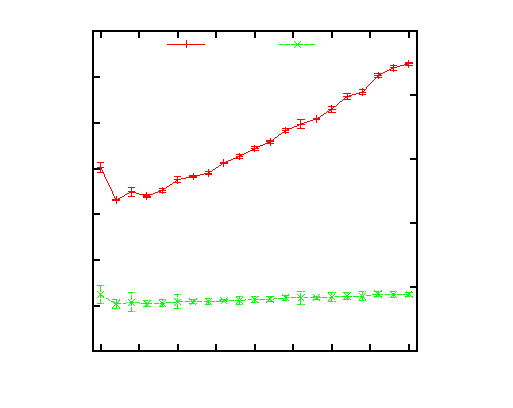
\includegraphics{CumulativeSumSkew_n8as16_Select_L2CH}}%
    \gplfronttext
  \end{picture}%
\endgroup

	\caption{Level 2 Data Cache Hits \& Hit Rate}
	\label{fig:CumulativeSumSkew_n8as16_Select_L2CH}
\end{subfigure}
\hfill
\begin{subfigure}{0.48\textwidth}
	% GNUPLOT: LaTeX picture with Postscript
\begingroup
  \makeatletter
  \providecommand\color[2][]{%
    \GenericError{(gnuplot) \space\space\space\@spaces}{%
      Package color not loaded in conjunction with
      terminal option `colourtext'%
    }{See the gnuplot documentation for explanation.%
    }{Either use 'blacktext' in gnuplot or load the package
      color.sty in LaTeX.}%
    \renewcommand\color[2][]{}%
  }%
  \providecommand\includegraphics[2][]{%
    \GenericError{(gnuplot) \space\space\space\@spaces}{%
      Package graphicx or graphics not loaded%
    }{See the gnuplot documentation for explanation.%
    }{The gnuplot epslatex terminal needs graphicx.sty or graphics.sty.}%
    \renewcommand\includegraphics[2][]{}%
  }%
  \providecommand\rotatebox[2]{#2}%
  \@ifundefined{ifGPcolor}{%
    \newif\ifGPcolor
    \GPcolortrue
  }{}%
  \@ifundefined{ifGPblacktext}{%
    \newif\ifGPblacktext
    \GPblacktexttrue
  }{}%
  % define a \g@addto@macro without @ in the name:
  \let\gplgaddtomacro\g@addto@macro
  % define empty templates for all commands taking text:
  \gdef\gplbacktext{}%
  \gdef\gplfronttext{}%
  \makeatother
  \ifGPblacktext
    % no textcolor at all
    \def\colorrgb#1{}%
    \def\colorgray#1{}%
  \else
    % gray or color?
    \ifGPcolor
      \def\colorrgb#1{\color[rgb]{#1}}%
      \def\colorgray#1{\color[gray]{#1}}%
      \expandafter\def\csname LTw\endcsname{\color{white}}%
      \expandafter\def\csname LTb\endcsname{\color{black}}%
      \expandafter\def\csname LTa\endcsname{\color{black}}%
      \expandafter\def\csname LT0\endcsname{\color[rgb]{1,0,0}}%
      \expandafter\def\csname LT1\endcsname{\color[rgb]{0,1,0}}%
      \expandafter\def\csname LT2\endcsname{\color[rgb]{0,0,1}}%
      \expandafter\def\csname LT3\endcsname{\color[rgb]{1,0,1}}%
      \expandafter\def\csname LT4\endcsname{\color[rgb]{0,1,1}}%
      \expandafter\def\csname LT5\endcsname{\color[rgb]{1,1,0}}%
      \expandafter\def\csname LT6\endcsname{\color[rgb]{0,0,0}}%
      \expandafter\def\csname LT7\endcsname{\color[rgb]{1,0.3,0}}%
      \expandafter\def\csname LT8\endcsname{\color[rgb]{0.5,0.5,0.5}}%
    \else
      % gray
      \def\colorrgb#1{\color{black}}%
      \def\colorgray#1{\color[gray]{#1}}%
      \expandafter\def\csname LTw\endcsname{\color{white}}%
      \expandafter\def\csname LTb\endcsname{\color{black}}%
      \expandafter\def\csname LTa\endcsname{\color{black}}%
      \expandafter\def\csname LT0\endcsname{\color{black}}%
      \expandafter\def\csname LT1\endcsname{\color{black}}%
      \expandafter\def\csname LT2\endcsname{\color{black}}%
      \expandafter\def\csname LT3\endcsname{\color{black}}%
      \expandafter\def\csname LT4\endcsname{\color{black}}%
      \expandafter\def\csname LT5\endcsname{\color{black}}%
      \expandafter\def\csname LT6\endcsname{\color{black}}%
      \expandafter\def\csname LT7\endcsname{\color{black}}%
      \expandafter\def\csname LT8\endcsname{\color{black}}%
    \fi
  \fi
  \setlength{\unitlength}{0.0500bp}%
  \begin{picture}(4608.00,3600.00)%
    \gplgaddtomacro\gplbacktext{%
      \csname LTb\endcsname%
      \put(804,384){\makebox(0,0)[r]{\strut{} 0}}%
      \put(804,768){\makebox(0,0)[r]{\strut{} 500000}}%
      \put(804,1152){\makebox(0,0)[r]{\strut{} 1e+06}}%
      \put(804,1536){\makebox(0,0)[r]{\strut{} 1.5e+06}}%
      \put(804,1920){\makebox(0,0)[r]{\strut{} 2e+06}}%
      \put(804,2303){\makebox(0,0)[r]{\strut{} 2.5e+06}}%
      \put(804,2687){\makebox(0,0)[r]{\strut{} 3e+06}}%
      \put(804,3071){\makebox(0,0)[r]{\strut{} 3.5e+06}}%
      \put(804,3455){\makebox(0,0)[r]{\strut{} 4e+06}}%
      \put(960,264){\makebox(0,0){\strut{} 2}}%
      \put(1378,264){\makebox(0,0){\strut{} 2.5}}%
      \put(1797,264){\makebox(0,0){\strut{} 3}}%
      \put(2215,264){\makebox(0,0){\strut{} 3.5}}%
      \put(2634,264){\makebox(0,0){\strut{} 4}}%
      \put(3052,264){\makebox(0,0){\strut{} 4.5}}%
      \put(3470,264){\makebox(0,0){\strut{} 5}}%
      \put(3889,264){\makebox(0,0){\strut{} 5.5}}%
      \put(4307,264){\makebox(0,0){\strut{} 6}}%
      \put(96,1919){\rotatebox{-270}{\makebox(0,0){\strut{}Branches Executed}}}%
      \put(2633,84){\makebox(0,0){\strut{}Skew Parameter}}%
    }%
    \gplgaddtomacro\gplfronttext{%
    }%
    \gplbacktext
    \put(0,0){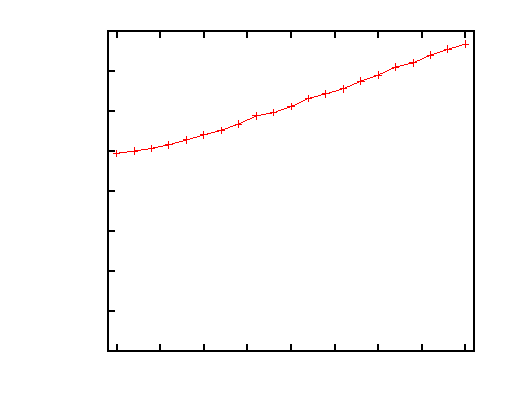
\includegraphics{CumulativeSumSkew_n8as16_Select_BMExe}}%
    \gplfronttext
  \end{picture}%
\endgroup

	\caption{Branches Executed}
	\label{fig:CumulativeSumSkew_n8as16_Select_BMExe}
\end{subfigure}

\begin{subfigure}{0.48\textwidth}
	% GNUPLOT: LaTeX picture with Postscript
\begingroup
  \makeatletter
  \providecommand\color[2][]{%
    \GenericError{(gnuplot) \space\space\space\@spaces}{%
      Package color not loaded in conjunction with
      terminal option `colourtext'%
    }{See the gnuplot documentation for explanation.%
    }{Either use 'blacktext' in gnuplot or load the package
      color.sty in LaTeX.}%
    \renewcommand\color[2][]{}%
  }%
  \providecommand\includegraphics[2][]{%
    \GenericError{(gnuplot) \space\space\space\@spaces}{%
      Package graphicx or graphics not loaded%
    }{See the gnuplot documentation for explanation.%
    }{The gnuplot epslatex terminal needs graphicx.sty or graphics.sty.}%
    \renewcommand\includegraphics[2][]{}%
  }%
  \providecommand\rotatebox[2]{#2}%
  \@ifundefined{ifGPcolor}{%
    \newif\ifGPcolor
    \GPcolortrue
  }{}%
  \@ifundefined{ifGPblacktext}{%
    \newif\ifGPblacktext
    \GPblacktexttrue
  }{}%
  % define a \g@addto@macro without @ in the name:
  \let\gplgaddtomacro\g@addto@macro
  % define empty templates for all commands taking text:
  \gdef\gplbacktext{}%
  \gdef\gplfronttext{}%
  \makeatother
  \ifGPblacktext
    % no textcolor at all
    \def\colorrgb#1{}%
    \def\colorgray#1{}%
  \else
    % gray or color?
    \ifGPcolor
      \def\colorrgb#1{\color[rgb]{#1}}%
      \def\colorgray#1{\color[gray]{#1}}%
      \expandafter\def\csname LTw\endcsname{\color{white}}%
      \expandafter\def\csname LTb\endcsname{\color{black}}%
      \expandafter\def\csname LTa\endcsname{\color{black}}%
      \expandafter\def\csname LT0\endcsname{\color[rgb]{1,0,0}}%
      \expandafter\def\csname LT1\endcsname{\color[rgb]{0,1,0}}%
      \expandafter\def\csname LT2\endcsname{\color[rgb]{0,0,1}}%
      \expandafter\def\csname LT3\endcsname{\color[rgb]{1,0,1}}%
      \expandafter\def\csname LT4\endcsname{\color[rgb]{0,1,1}}%
      \expandafter\def\csname LT5\endcsname{\color[rgb]{1,1,0}}%
      \expandafter\def\csname LT6\endcsname{\color[rgb]{0,0,0}}%
      \expandafter\def\csname LT7\endcsname{\color[rgb]{1,0.3,0}}%
      \expandafter\def\csname LT8\endcsname{\color[rgb]{0.5,0.5,0.5}}%
    \else
      % gray
      \def\colorrgb#1{\color{black}}%
      \def\colorgray#1{\color[gray]{#1}}%
      \expandafter\def\csname LTw\endcsname{\color{white}}%
      \expandafter\def\csname LTb\endcsname{\color{black}}%
      \expandafter\def\csname LTa\endcsname{\color{black}}%
      \expandafter\def\csname LT0\endcsname{\color{black}}%
      \expandafter\def\csname LT1\endcsname{\color{black}}%
      \expandafter\def\csname LT2\endcsname{\color{black}}%
      \expandafter\def\csname LT3\endcsname{\color{black}}%
      \expandafter\def\csname LT4\endcsname{\color{black}}%
      \expandafter\def\csname LT5\endcsname{\color{black}}%
      \expandafter\def\csname LT6\endcsname{\color{black}}%
      \expandafter\def\csname LT7\endcsname{\color{black}}%
      \expandafter\def\csname LT8\endcsname{\color{black}}%
    \fi
  \fi
  \setlength{\unitlength}{0.0500bp}%
  \begin{picture}(4608.00,3600.00)%
    \gplgaddtomacro\gplbacktext{%
      \csname LTb\endcsname%
      \put(732,384){\makebox(0,0)[r]{\strut{} 0}}%
      \put(732,998){\makebox(0,0)[r]{\strut{} 100000}}%
      \put(732,1612){\makebox(0,0)[r]{\strut{} 200000}}%
      \put(732,2227){\makebox(0,0)[r]{\strut{} 300000}}%
      \put(732,2841){\makebox(0,0)[r]{\strut{} 400000}}%
      \put(732,3455){\makebox(0,0)[r]{\strut{} 500000}}%
      \put(876,264){\makebox(0,0){\strut{} 2}}%
      \put(1238,264){\makebox(0,0){\strut{} 2.5}}%
      \put(1599,264){\makebox(0,0){\strut{} 3}}%
      \put(1960,264){\makebox(0,0){\strut{} 3.5}}%
      \put(2322,264){\makebox(0,0){\strut{} 4}}%
      \put(2683,264){\makebox(0,0){\strut{} 4.5}}%
      \put(3044,264){\makebox(0,0){\strut{} 5}}%
      \put(3405,264){\makebox(0,0){\strut{} 5.5}}%
      \put(3767,264){\makebox(0,0){\strut{} 6}}%
      \put(3911,384){\makebox(0,0)[l]{\strut{} 0}}%
      \put(3911,998){\makebox(0,0)[l]{\strut{} 0.2}}%
      \put(3911,1612){\makebox(0,0)[l]{\strut{} 0.4}}%
      \put(3911,2227){\makebox(0,0)[l]{\strut{} 0.6}}%
      \put(3911,2841){\makebox(0,0)[l]{\strut{} 0.8}}%
      \put(3911,3455){\makebox(0,0)[l]{\strut{} 1}}%
      \put(96,1919){\rotatebox{-270}{\makebox(0,0){\strut{}Branch Mispredictions}}}%
      \put(4330,1919){\rotatebox{-270}{\makebox(0,0){\strut{}Branch Misprediction Rate}}}%
      \put(2321,84){\makebox(0,0){\strut{}Skew Parameter}}%
    }%
    \gplgaddtomacro\gplfronttext{%
      \csname LTb\endcsname%
      \put(2676,3332){\makebox(0,0)[r]{\strut{}Branch Mispredictions}}%
      \csname LTb\endcsname%
      \put(2676,3212){\makebox(0,0)[r]{\strut{}Branch Misprediction Rate}}%
    }%
    \gplbacktext
    \put(0,0){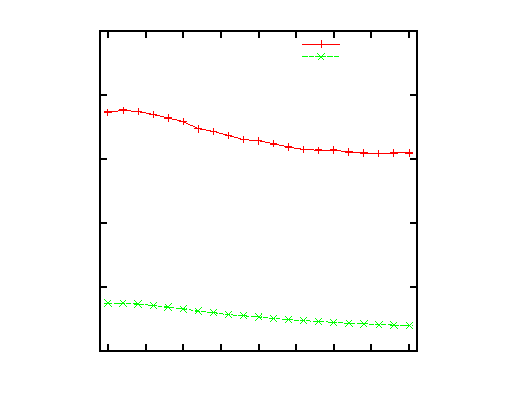
\includegraphics{CumulativeSumSkew_n8as16_Select_BM}}%
    \gplfronttext
  \end{picture}%
\endgroup

	\caption{Branch Mispredictions}
	\label{fig:CumulativeSumSkew_n8as16_Select_BM}
\end{subfigure}
\hfill
\begin{subfigure}{0.48\textwidth}
	% GNUPLOT: LaTeX picture with Postscript
\begingroup
  \makeatletter
  \providecommand\color[2][]{%
    \GenericError{(gnuplot) \space\space\space\@spaces}{%
      Package color not loaded in conjunction with
      terminal option `colourtext'%
    }{See the gnuplot documentation for explanation.%
    }{Either use 'blacktext' in gnuplot or load the package
      color.sty in LaTeX.}%
    \renewcommand\color[2][]{}%
  }%
  \providecommand\includegraphics[2][]{%
    \GenericError{(gnuplot) \space\space\space\@spaces}{%
      Package graphicx or graphics not loaded%
    }{See the gnuplot documentation for explanation.%
    }{The gnuplot epslatex terminal needs graphicx.sty or graphics.sty.}%
    \renewcommand\includegraphics[2][]{}%
  }%
  \providecommand\rotatebox[2]{#2}%
  \@ifundefined{ifGPcolor}{%
    \newif\ifGPcolor
    \GPcolortrue
  }{}%
  \@ifundefined{ifGPblacktext}{%
    \newif\ifGPblacktext
    \GPblacktexttrue
  }{}%
  % define a \g@addto@macro without @ in the name:
  \let\gplgaddtomacro\g@addto@macro
  % define empty templates for all commands taking text:
  \gdef\gplbacktext{}%
  \gdef\gplfronttext{}%
  \makeatother
  \ifGPblacktext
    % no textcolor at all
    \def\colorrgb#1{}%
    \def\colorgray#1{}%
  \else
    % gray or color?
    \ifGPcolor
      \def\colorrgb#1{\color[rgb]{#1}}%
      \def\colorgray#1{\color[gray]{#1}}%
      \expandafter\def\csname LTw\endcsname{\color{white}}%
      \expandafter\def\csname LTb\endcsname{\color{black}}%
      \expandafter\def\csname LTa\endcsname{\color{black}}%
      \expandafter\def\csname LT0\endcsname{\color[rgb]{1,0,0}}%
      \expandafter\def\csname LT1\endcsname{\color[rgb]{0,1,0}}%
      \expandafter\def\csname LT2\endcsname{\color[rgb]{0,0,1}}%
      \expandafter\def\csname LT3\endcsname{\color[rgb]{1,0,1}}%
      \expandafter\def\csname LT4\endcsname{\color[rgb]{0,1,1}}%
      \expandafter\def\csname LT5\endcsname{\color[rgb]{1,1,0}}%
      \expandafter\def\csname LT6\endcsname{\color[rgb]{0,0,0}}%
      \expandafter\def\csname LT7\endcsname{\color[rgb]{1,0.3,0}}%
      \expandafter\def\csname LT8\endcsname{\color[rgb]{0.5,0.5,0.5}}%
    \else
      % gray
      \def\colorrgb#1{\color{black}}%
      \def\colorgray#1{\color[gray]{#1}}%
      \expandafter\def\csname LTw\endcsname{\color{white}}%
      \expandafter\def\csname LTb\endcsname{\color{black}}%
      \expandafter\def\csname LTa\endcsname{\color{black}}%
      \expandafter\def\csname LT0\endcsname{\color{black}}%
      \expandafter\def\csname LT1\endcsname{\color{black}}%
      \expandafter\def\csname LT2\endcsname{\color{black}}%
      \expandafter\def\csname LT3\endcsname{\color{black}}%
      \expandafter\def\csname LT4\endcsname{\color{black}}%
      \expandafter\def\csname LT5\endcsname{\color{black}}%
      \expandafter\def\csname LT6\endcsname{\color{black}}%
      \expandafter\def\csname LT7\endcsname{\color{black}}%
      \expandafter\def\csname LT8\endcsname{\color{black}}%
    \fi
  \fi
  \setlength{\unitlength}{0.0500bp}%
  \begin{picture}(4608.00,3600.00)%
    \gplgaddtomacro\gplbacktext{%
      \csname LTb\endcsname%
      \put(660,384){\makebox(0,0)[r]{\strut{} 0}}%
      \put(660,725){\makebox(0,0)[r]{\strut{} 2000}}%
      \put(660,1066){\makebox(0,0)[r]{\strut{} 4000}}%
      \put(660,1408){\makebox(0,0)[r]{\strut{} 6000}}%
      \put(660,1749){\makebox(0,0)[r]{\strut{} 8000}}%
      \put(660,2090){\makebox(0,0)[r]{\strut{} 10000}}%
      \put(660,2431){\makebox(0,0)[r]{\strut{} 12000}}%
      \put(660,2773){\makebox(0,0)[r]{\strut{} 14000}}%
      \put(660,3114){\makebox(0,0)[r]{\strut{} 16000}}%
      \put(660,3455){\makebox(0,0)[r]{\strut{} 18000}}%
      \put(819,264){\makebox(0,0){\strut{} 2}}%
      \put(1255,264){\makebox(0,0){\strut{} 2.5}}%
      \put(1690,264){\makebox(0,0){\strut{} 3}}%
      \put(2126,264){\makebox(0,0){\strut{} 3.5}}%
      \put(2562,264){\makebox(0,0){\strut{} 4}}%
      \put(2997,264){\makebox(0,0){\strut{} 4.5}}%
      \put(3433,264){\makebox(0,0){\strut{} 5}}%
      \put(3868,264){\makebox(0,0){\strut{} 5.5}}%
      \put(4304,264){\makebox(0,0){\strut{} 6}}%
      \put(96,1919){\rotatebox{-270}{\makebox(0,0){\strut{}Translation Lookaside Buffer Misses}}}%
      \put(2561,84){\makebox(0,0){\strut{}Skew Parameter}}%
    }%
    \gplgaddtomacro\gplfronttext{%
    }%
    \gplbacktext
    \put(0,0){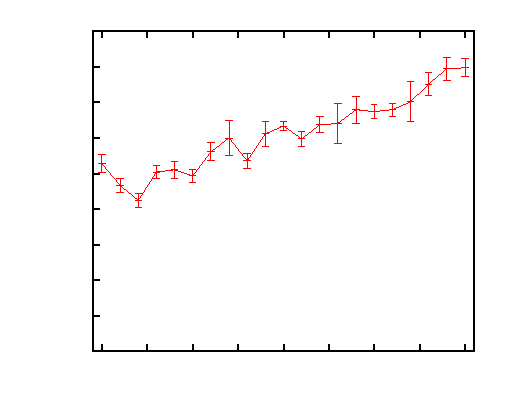
\includegraphics{CumulativeSumSkew_n8as16_Select_TLBM}}%
    \gplfronttext
  \end{picture}%
\endgroup

	\caption{Translation Lookaside Buffer Misses}
	\label{fig:CumulativeSumSkew_n8as16_Select_TLBM}
\end{subfigure}

\caption{Measurements for Select Queries on CumulativeSum for various skew.}
\label{fig:CumulativeSumSkew_n8as16_Select}
\end{figure}

\restoregeometry

\iffalse
\newgeometry{left=2cm,right=2cm, top=2cm, bottom=3cm}

\begin{figure}\tiny
\begin{subfigure}{0.48\textwidth}
	% GNUPLOT: LaTeX picture with Postscript
\begingroup
  \makeatletter
  \providecommand\color[2][]{%
    \GenericError{(gnuplot) \space\space\space\@spaces}{%
      Package color not loaded in conjunction with
      terminal option `colourtext'%
    }{See the gnuplot documentation for explanation.%
    }{Either use 'blacktext' in gnuplot or load the package
      color.sty in LaTeX.}%
    \renewcommand\color[2][]{}%
  }%
  \providecommand\includegraphics[2][]{%
    \GenericError{(gnuplot) \space\space\space\@spaces}{%
      Package graphicx or graphics not loaded%
    }{See the gnuplot documentation for explanation.%
    }{The gnuplot epslatex terminal needs graphicx.sty or graphics.sty.}%
    \renewcommand\includegraphics[2][]{}%
  }%
  \providecommand\rotatebox[2]{#2}%
  \@ifundefined{ifGPcolor}{%
    \newif\ifGPcolor
    \GPcolortrue
  }{}%
  \@ifundefined{ifGPblacktext}{%
    \newif\ifGPblacktext
    \GPblacktexttrue
  }{}%
  % define a \g@addto@macro without @ in the name:
  \let\gplgaddtomacro\g@addto@macro
  % define empty templates for all commands taking text:
  \gdef\gplbacktext{}%
  \gdef\gplfronttext{}%
  \makeatother
  \ifGPblacktext
    % no textcolor at all
    \def\colorrgb#1{}%
    \def\colorgray#1{}%
  \else
    % gray or color?
    \ifGPcolor
      \def\colorrgb#1{\color[rgb]{#1}}%
      \def\colorgray#1{\color[gray]{#1}}%
      \expandafter\def\csname LTw\endcsname{\color{white}}%
      \expandafter\def\csname LTb\endcsname{\color{black}}%
      \expandafter\def\csname LTa\endcsname{\color{black}}%
      \expandafter\def\csname LT0\endcsname{\color[rgb]{1,0,0}}%
      \expandafter\def\csname LT1\endcsname{\color[rgb]{0,1,0}}%
      \expandafter\def\csname LT2\endcsname{\color[rgb]{0,0,1}}%
      \expandafter\def\csname LT3\endcsname{\color[rgb]{1,0,1}}%
      \expandafter\def\csname LT4\endcsname{\color[rgb]{0,1,1}}%
      \expandafter\def\csname LT5\endcsname{\color[rgb]{1,1,0}}%
      \expandafter\def\csname LT6\endcsname{\color[rgb]{0,0,0}}%
      \expandafter\def\csname LT7\endcsname{\color[rgb]{1,0.3,0}}%
      \expandafter\def\csname LT8\endcsname{\color[rgb]{0.5,0.5,0.5}}%
    \else
      % gray
      \def\colorrgb#1{\color{black}}%
      \def\colorgray#1{\color[gray]{#1}}%
      \expandafter\def\csname LTw\endcsname{\color{white}}%
      \expandafter\def\csname LTb\endcsname{\color{black}}%
      \expandafter\def\csname LTa\endcsname{\color{black}}%
      \expandafter\def\csname LT0\endcsname{\color{black}}%
      \expandafter\def\csname LT1\endcsname{\color{black}}%
      \expandafter\def\csname LT2\endcsname{\color{black}}%
      \expandafter\def\csname LT3\endcsname{\color{black}}%
      \expandafter\def\csname LT4\endcsname{\color{black}}%
      \expandafter\def\csname LT5\endcsname{\color{black}}%
      \expandafter\def\csname LT6\endcsname{\color{black}}%
      \expandafter\def\csname LT7\endcsname{\color{black}}%
      \expandafter\def\csname LT8\endcsname{\color{black}}%
    \fi
  \fi
  \setlength{\unitlength}{0.0500bp}%
  \begin{picture}(4608.00,3600.00)%
    \gplgaddtomacro\gplbacktext{%
      \csname LTb\endcsname%
      \put(516,384){\makebox(0,0)[r]{\strut{} 0}}%
      \put(516,998){\makebox(0,0)[r]{\strut{} 0.5}}%
      \put(516,1612){\makebox(0,0)[r]{\strut{} 1}}%
      \put(516,2227){\makebox(0,0)[r]{\strut{} 1.5}}%
      \put(516,2841){\makebox(0,0)[r]{\strut{} 2}}%
      \put(516,3455){\makebox(0,0)[r]{\strut{} 2.5}}%
      \put(588,264){\makebox(0,0){\strut{} 2}}%
      \put(1063,264){\makebox(0,0){\strut{} 2.5}}%
      \put(1539,264){\makebox(0,0){\strut{} 3}}%
      \put(2014,264){\makebox(0,0){\strut{} 3.5}}%
      \put(2490,264){\makebox(0,0){\strut{} 4}}%
      \put(2965,264){\makebox(0,0){\strut{} 4.5}}%
      \put(3440,264){\makebox(0,0){\strut{} 5}}%
      \put(3916,264){\makebox(0,0){\strut{} 5.5}}%
      \put(4391,264){\makebox(0,0){\strut{} 6}}%
      \put(96,1919){\rotatebox{-270}{\makebox(0,0){\strut{}Wall Time (sec)}}}%
      \put(2489,84){\makebox(0,0){\strut{}Skew}}%
    }%
    \gplgaddtomacro\gplfronttext{%
      \csname LTb\endcsname%
      \put(1812,3332){\makebox(0,0)[r]{\strut{}NaiveInteger}}%
      \csname LTb\endcsname%
      \put(3459,3332){\makebox(0,0)[r]{\strut{}ControlledMemory}}%
    }%
    \gplbacktext
    \put(0,0){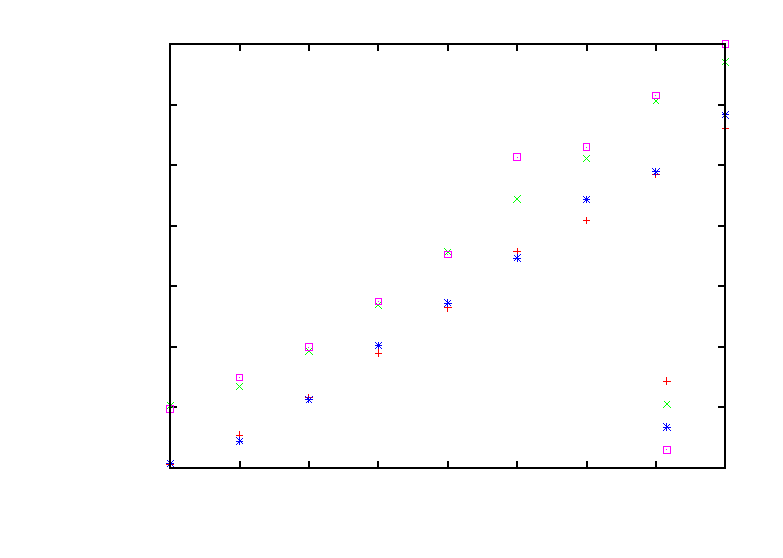
\includegraphics{naiveRankSkewRunningTime}}%
    \gplfronttext
  \end{picture}%
\endgroup

	\caption{Wall Time}
	\label{fig:NaiveRankSkewRunningTime}
\end{subfigure}
\hfill
\begin{subfigure}{0.48\textwidth}
	% GNUPLOT: LaTeX picture with Postscript
\begingroup
  \makeatletter
  \providecommand\color[2][]{%
    \GenericError{(gnuplot) \space\space\space\@spaces}{%
      Package color not loaded in conjunction with
      terminal option `colourtext'%
    }{See the gnuplot documentation for explanation.%
    }{Either use 'blacktext' in gnuplot or load the package
      color.sty in LaTeX.}%
    \renewcommand\color[2][]{}%
  }%
  \providecommand\includegraphics[2][]{%
    \GenericError{(gnuplot) \space\space\space\@spaces}{%
      Package graphicx or graphics not loaded%
    }{See the gnuplot documentation for explanation.%
    }{The gnuplot epslatex terminal needs graphicx.sty or graphics.sty.}%
    \renewcommand\includegraphics[2][]{}%
  }%
  \providecommand\rotatebox[2]{#2}%
  \@ifundefined{ifGPcolor}{%
    \newif\ifGPcolor
    \GPcolortrue
  }{}%
  \@ifundefined{ifGPblacktext}{%
    \newif\ifGPblacktext
    \GPblacktexttrue
  }{}%
  % define a \g@addto@macro without @ in the name:
  \let\gplgaddtomacro\g@addto@macro
  % define empty templates for all commands taking text:
  \gdef\gplbacktext{}%
  \gdef\gplfronttext{}%
  \makeatother
  \ifGPblacktext
    % no textcolor at all
    \def\colorrgb#1{}%
    \def\colorgray#1{}%
  \else
    % gray or color?
    \ifGPcolor
      \def\colorrgb#1{\color[rgb]{#1}}%
      \def\colorgray#1{\color[gray]{#1}}%
      \expandafter\def\csname LTw\endcsname{\color{white}}%
      \expandafter\def\csname LTb\endcsname{\color{black}}%
      \expandafter\def\csname LTa\endcsname{\color{black}}%
      \expandafter\def\csname LT0\endcsname{\color[rgb]{1,0,0}}%
      \expandafter\def\csname LT1\endcsname{\color[rgb]{0,1,0}}%
      \expandafter\def\csname LT2\endcsname{\color[rgb]{0,0,1}}%
      \expandafter\def\csname LT3\endcsname{\color[rgb]{1,0,1}}%
      \expandafter\def\csname LT4\endcsname{\color[rgb]{0,1,1}}%
      \expandafter\def\csname LT5\endcsname{\color[rgb]{1,1,0}}%
      \expandafter\def\csname LT6\endcsname{\color[rgb]{0,0,0}}%
      \expandafter\def\csname LT7\endcsname{\color[rgb]{1,0.3,0}}%
      \expandafter\def\csname LT8\endcsname{\color[rgb]{0.5,0.5,0.5}}%
    \else
      % gray
      \def\colorrgb#1{\color{black}}%
      \def\colorgray#1{\color[gray]{#1}}%
      \expandafter\def\csname LTw\endcsname{\color{white}}%
      \expandafter\def\csname LTb\endcsname{\color{black}}%
      \expandafter\def\csname LTa\endcsname{\color{black}}%
      \expandafter\def\csname LT0\endcsname{\color{black}}%
      \expandafter\def\csname LT1\endcsname{\color{black}}%
      \expandafter\def\csname LT2\endcsname{\color{black}}%
      \expandafter\def\csname LT3\endcsname{\color{black}}%
      \expandafter\def\csname LT4\endcsname{\color{black}}%
      \expandafter\def\csname LT5\endcsname{\color{black}}%
      \expandafter\def\csname LT6\endcsname{\color{black}}%
      \expandafter\def\csname LT7\endcsname{\color{black}}%
      \expandafter\def\csname LT8\endcsname{\color{black}}%
    \fi
  \fi
  \setlength{\unitlength}{0.0500bp}%
  \begin{picture}(4608.00,3600.00)%
    \gplgaddtomacro\gplbacktext{%
      \csname LTb\endcsname%
      \put(804,384){\makebox(0,0)[r]{\strut{} 0}}%
      \put(804,725){\makebox(0,0)[r]{\strut{} 2e-06}}%
      \put(804,1066){\makebox(0,0)[r]{\strut{} 4e-06}}%
      \put(804,1408){\makebox(0,0)[r]{\strut{} 6e-06}}%
      \put(804,1749){\makebox(0,0)[r]{\strut{} 8e-06}}%
      \put(804,2090){\makebox(0,0)[r]{\strut{} 1e-05}}%
      \put(804,2431){\makebox(0,0)[r]{\strut{} 1.2e-05}}%
      \put(804,2773){\makebox(0,0)[r]{\strut{} 1.4e-05}}%
      \put(804,3114){\makebox(0,0)[r]{\strut{} 1.6e-05}}%
      \put(804,3455){\makebox(0,0)[r]{\strut{} 1.8e-05}}%
      \put(876,264){\makebox(0,0){\strut{} 2}}%
      \put(1315,264){\makebox(0,0){\strut{} 2.5}}%
      \put(1755,264){\makebox(0,0){\strut{} 3}}%
      \put(2194,264){\makebox(0,0){\strut{} 3.5}}%
      \put(2634,264){\makebox(0,0){\strut{} 4}}%
      \put(3073,264){\makebox(0,0){\strut{} 4.5}}%
      \put(3512,264){\makebox(0,0){\strut{} 5}}%
      \put(3952,264){\makebox(0,0){\strut{} 5.5}}%
      \put(4391,264){\makebox(0,0){\strut{} 6}}%
      \put(96,1919){\rotatebox{-270}{\makebox(0,0){\strut{}Branch Misprediction Rate}}}%
      \put(2633,84){\makebox(0,0){\strut{}Skew}}%
    }%
    \gplgaddtomacro\gplfronttext{%
      \csname LTb\endcsname%
      \put(1889,3332){\makebox(0,0)[r]{\strut{}Naive}}%
      \csname LTb\endcsname%
      \put(3824,3332){\makebox(0,0)[r]{\strut{}ControlledNodeMemory}}%
    }%
    \gplbacktext
    \put(0,0){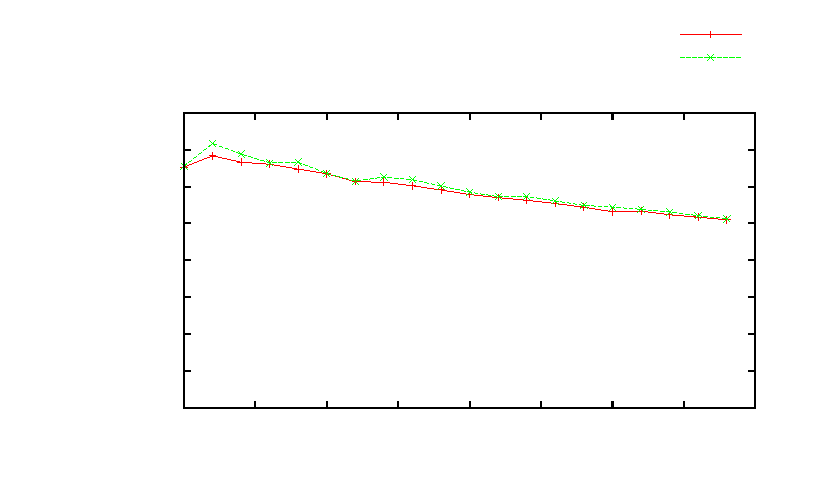
\includegraphics{NaiveVsControlledNodeMemorySkewRankQuery_BMrate}}%
    \gplfronttext
  \end{picture}%
\endgroup

	\caption{Branch Misprediction Rate}
	\label{fig:NaiveVsControlledNodeMemorySkewRankQueryBMrate}
\end{subfigure}


\begin{subfigure}{0.48\textwidth}
	% GNUPLOT: LaTeX picture with Postscript
\begingroup
  \makeatletter
  \providecommand\color[2][]{%
    \GenericError{(gnuplot) \space\space\space\@spaces}{%
      Package color not loaded in conjunction with
      terminal option `colourtext'%
    }{See the gnuplot documentation for explanation.%
    }{Either use 'blacktext' in gnuplot or load the package
      color.sty in LaTeX.}%
    \renewcommand\color[2][]{}%
  }%
  \providecommand\includegraphics[2][]{%
    \GenericError{(gnuplot) \space\space\space\@spaces}{%
      Package graphicx or graphics not loaded%
    }{See the gnuplot documentation for explanation.%
    }{The gnuplot epslatex terminal needs graphicx.sty or graphics.sty.}%
    \renewcommand\includegraphics[2][]{}%
  }%
  \providecommand\rotatebox[2]{#2}%
  \@ifundefined{ifGPcolor}{%
    \newif\ifGPcolor
    \GPcolortrue
  }{}%
  \@ifundefined{ifGPblacktext}{%
    \newif\ifGPblacktext
    \GPblacktexttrue
  }{}%
  % define a \g@addto@macro without @ in the name:
  \let\gplgaddtomacro\g@addto@macro
  % define empty templates for all commands taking text:
  \gdef\gplbacktext{}%
  \gdef\gplfronttext{}%
  \makeatother
  \ifGPblacktext
    % no textcolor at all
    \def\colorrgb#1{}%
    \def\colorgray#1{}%
  \else
    % gray or color?
    \ifGPcolor
      \def\colorrgb#1{\color[rgb]{#1}}%
      \def\colorgray#1{\color[gray]{#1}}%
      \expandafter\def\csname LTw\endcsname{\color{white}}%
      \expandafter\def\csname LTb\endcsname{\color{black}}%
      \expandafter\def\csname LTa\endcsname{\color{black}}%
      \expandafter\def\csname LT0\endcsname{\color[rgb]{1,0,0}}%
      \expandafter\def\csname LT1\endcsname{\color[rgb]{0,1,0}}%
      \expandafter\def\csname LT2\endcsname{\color[rgb]{0,0,1}}%
      \expandafter\def\csname LT3\endcsname{\color[rgb]{1,0,1}}%
      \expandafter\def\csname LT4\endcsname{\color[rgb]{0,1,1}}%
      \expandafter\def\csname LT5\endcsname{\color[rgb]{1,1,0}}%
      \expandafter\def\csname LT6\endcsname{\color[rgb]{0,0,0}}%
      \expandafter\def\csname LT7\endcsname{\color[rgb]{1,0.3,0}}%
      \expandafter\def\csname LT8\endcsname{\color[rgb]{0.5,0.5,0.5}}%
    \else
      % gray
      \def\colorrgb#1{\color{black}}%
      \def\colorgray#1{\color[gray]{#1}}%
      \expandafter\def\csname LTw\endcsname{\color{white}}%
      \expandafter\def\csname LTb\endcsname{\color{black}}%
      \expandafter\def\csname LTa\endcsname{\color{black}}%
      \expandafter\def\csname LT0\endcsname{\color{black}}%
      \expandafter\def\csname LT1\endcsname{\color{black}}%
      \expandafter\def\csname LT2\endcsname{\color{black}}%
      \expandafter\def\csname LT3\endcsname{\color{black}}%
      \expandafter\def\csname LT4\endcsname{\color{black}}%
      \expandafter\def\csname LT5\endcsname{\color{black}}%
      \expandafter\def\csname LT6\endcsname{\color{black}}%
      \expandafter\def\csname LT7\endcsname{\color{black}}%
      \expandafter\def\csname LT8\endcsname{\color{black}}%
    \fi
  \fi
  \setlength{\unitlength}{0.0500bp}%
  \begin{picture}(7488.00,4752.00)%
    \gplgaddtomacro\gplbacktext{%
      \csname LTb\endcsname%
      \put(1474,704){\makebox(0,0)[r]{\strut{} 0}}%
      \put(1474,1150){\makebox(0,0)[r]{\strut{} 5e+06}}%
      \put(1474,1596){\makebox(0,0)[r]{\strut{} 1e+07}}%
      \put(1474,2042){\makebox(0,0)[r]{\strut{} 1.5e+07}}%
      \put(1474,2489){\makebox(0,0)[r]{\strut{} 2e+07}}%
      \put(1474,2935){\makebox(0,0)[r]{\strut{} 2.5e+07}}%
      \put(1474,3381){\makebox(0,0)[r]{\strut{} 3e+07}}%
      \put(1474,3827){\makebox(0,0)[r]{\strut{} 3.5e+07}}%
      \put(1606,484){\makebox(0,0){\strut{} 2}}%
      \put(2292,484){\makebox(0,0){\strut{} 2.5}}%
      \put(2977,484){\makebox(0,0){\strut{} 3}}%
      \put(3663,484){\makebox(0,0){\strut{} 3.5}}%
      \put(4349,484){\makebox(0,0){\strut{} 4}}%
      \put(5034,484){\makebox(0,0){\strut{} 4.5}}%
      \put(5720,484){\makebox(0,0){\strut{} 5}}%
      \put(6405,484){\makebox(0,0){\strut{} 5.5}}%
      \put(7091,484){\makebox(0,0){\strut{} 6}}%
      \put(176,2265){\rotatebox{-270}{\makebox(0,0){\strut{}Cache Misses}}}%
      \put(4348,154){\makebox(0,0){\strut{}Skew}}%
    }%
    \gplgaddtomacro\gplfronttext{%
      \csname LTb\endcsname%
      \put(6236,4579){\makebox(0,0)[r]{\strut{}Naive L1 $mr\hat{\sigma}=$0.041 $avg\hat{\sigma}=$0.02}}%
      \csname LTb\endcsname%
      \put(6236,4359){\makebox(0,0)[r]{\strut{}ControlledNodeMemory L1 $mr\hat{\sigma}=$0.046 $avg\hat{\sigma}=$0.02}}%
    }%
    \gplbacktext
    \put(0,0){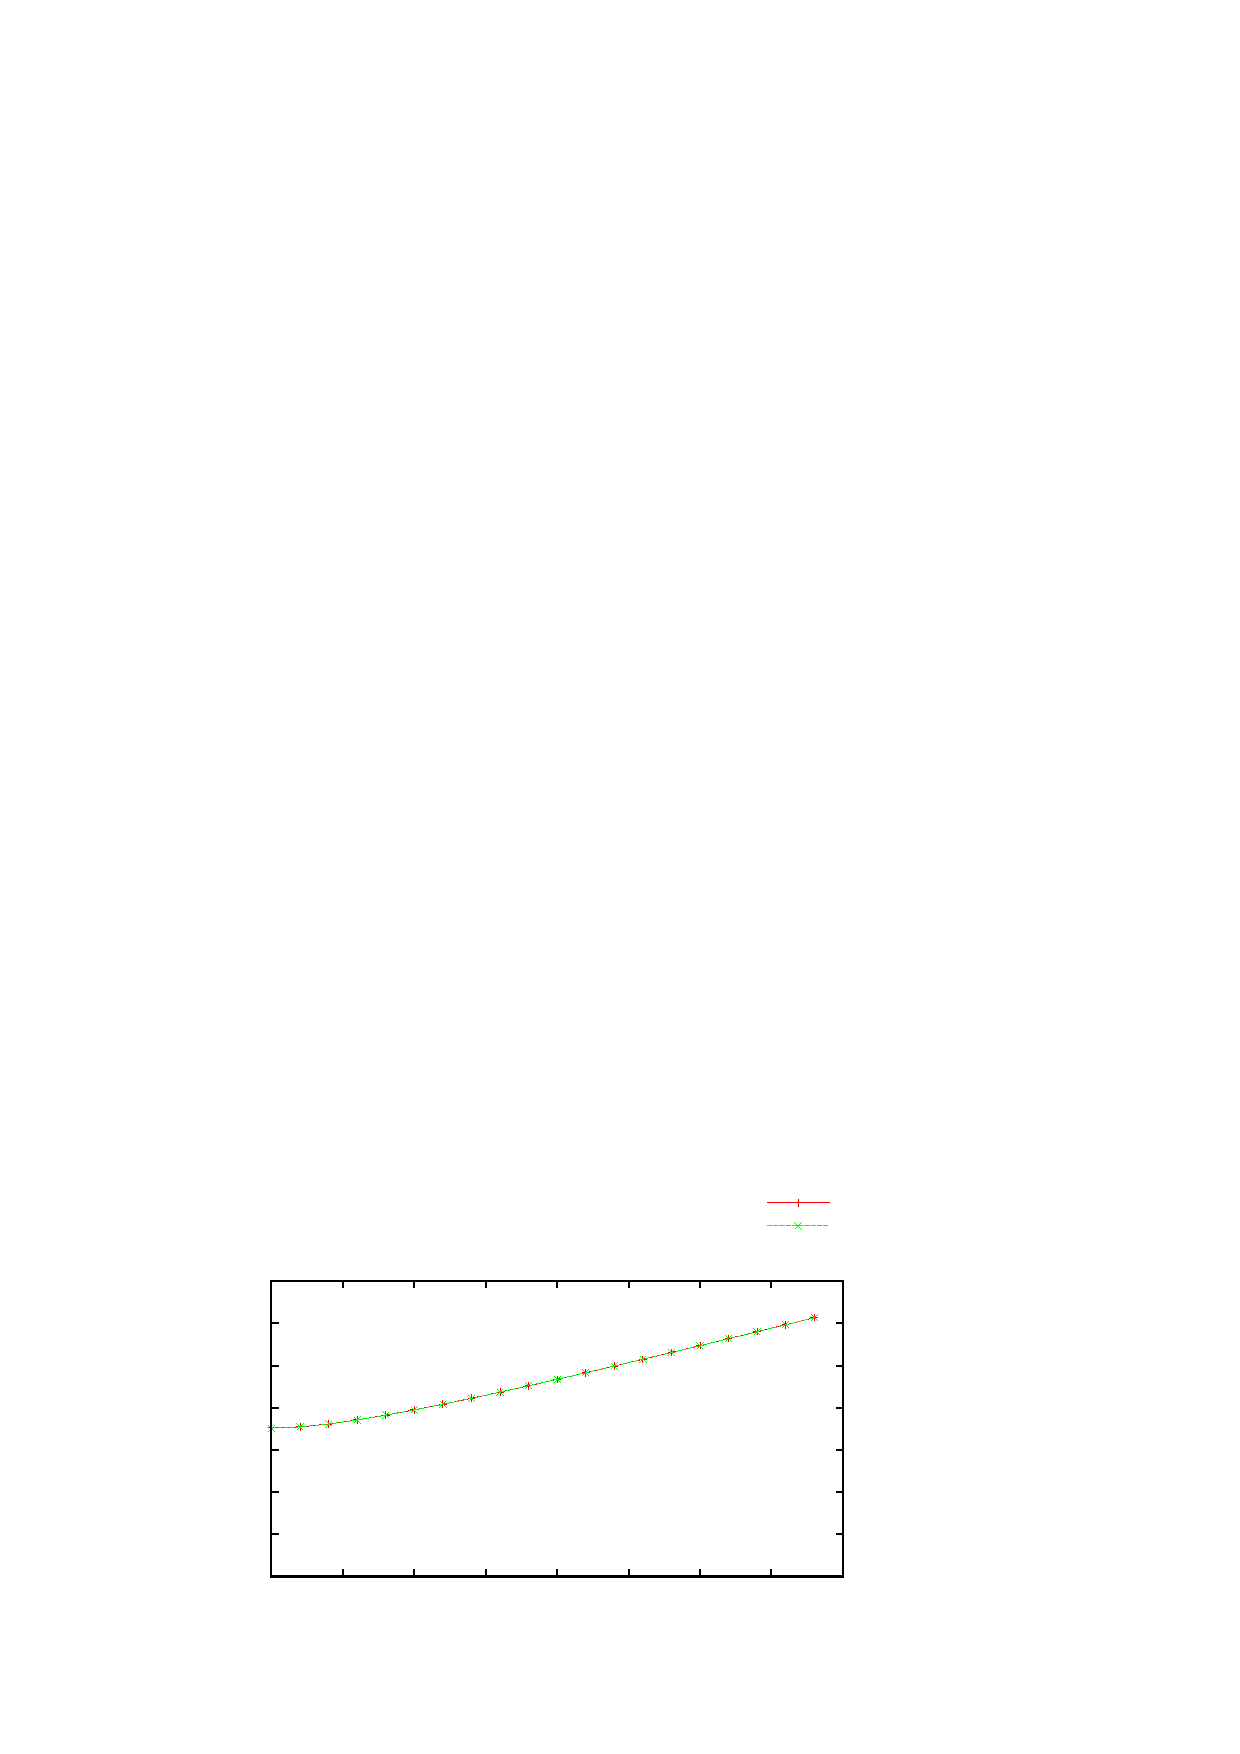
\includegraphics{L1NaiveVsControlledNodeMemorySkewRankQueryCacheMisses}}%
    \gplfronttext
  \end{picture}%
\endgroup

	\caption{Level 1 Data Cache Misses}
	\label{fig:L1NaiveControlledNodeMemoryRankSkewCacheMisses}
\end{subfigure}
\hfill
\begin{subfigure}{0.48\textwidth}
 	% GNUPLOT: LaTeX picture with Postscript
\begingroup
  \makeatletter
  \providecommand\color[2][]{%
    \GenericError{(gnuplot) \space\space\space\@spaces}{%
      Package color not loaded in conjunction with
      terminal option `colourtext'%
    }{See the gnuplot documentation for explanation.%
    }{Either use 'blacktext' in gnuplot or load the package
      color.sty in LaTeX.}%
    \renewcommand\color[2][]{}%
  }%
  \providecommand\includegraphics[2][]{%
    \GenericError{(gnuplot) \space\space\space\@spaces}{%
      Package graphicx or graphics not loaded%
    }{See the gnuplot documentation for explanation.%
    }{The gnuplot epslatex terminal needs graphicx.sty or graphics.sty.}%
    \renewcommand\includegraphics[2][]{}%
  }%
  \providecommand\rotatebox[2]{#2}%
  \@ifundefined{ifGPcolor}{%
    \newif\ifGPcolor
    \GPcolortrue
  }{}%
  \@ifundefined{ifGPblacktext}{%
    \newif\ifGPblacktext
    \GPblacktexttrue
  }{}%
  % define a \g@addto@macro without @ in the name:
  \let\gplgaddtomacro\g@addto@macro
  % define empty templates for all commands taking text:
  \gdef\gplbacktext{}%
  \gdef\gplfronttext{}%
  \makeatother
  \ifGPblacktext
    % no textcolor at all
    \def\colorrgb#1{}%
    \def\colorgray#1{}%
  \else
    % gray or color?
    \ifGPcolor
      \def\colorrgb#1{\color[rgb]{#1}}%
      \def\colorgray#1{\color[gray]{#1}}%
      \expandafter\def\csname LTw\endcsname{\color{white}}%
      \expandafter\def\csname LTb\endcsname{\color{black}}%
      \expandafter\def\csname LTa\endcsname{\color{black}}%
      \expandafter\def\csname LT0\endcsname{\color[rgb]{1,0,0}}%
      \expandafter\def\csname LT1\endcsname{\color[rgb]{0,1,0}}%
      \expandafter\def\csname LT2\endcsname{\color[rgb]{0,0,1}}%
      \expandafter\def\csname LT3\endcsname{\color[rgb]{1,0,1}}%
      \expandafter\def\csname LT4\endcsname{\color[rgb]{0,1,1}}%
      \expandafter\def\csname LT5\endcsname{\color[rgb]{1,1,0}}%
      \expandafter\def\csname LT6\endcsname{\color[rgb]{0,0,0}}%
      \expandafter\def\csname LT7\endcsname{\color[rgb]{1,0.3,0}}%
      \expandafter\def\csname LT8\endcsname{\color[rgb]{0.5,0.5,0.5}}%
    \else
      % gray
      \def\colorrgb#1{\color{black}}%
      \def\colorgray#1{\color[gray]{#1}}%
      \expandafter\def\csname LTw\endcsname{\color{white}}%
      \expandafter\def\csname LTb\endcsname{\color{black}}%
      \expandafter\def\csname LTa\endcsname{\color{black}}%
      \expandafter\def\csname LT0\endcsname{\color{black}}%
      \expandafter\def\csname LT1\endcsname{\color{black}}%
      \expandafter\def\csname LT2\endcsname{\color{black}}%
      \expandafter\def\csname LT3\endcsname{\color{black}}%
      \expandafter\def\csname LT4\endcsname{\color{black}}%
      \expandafter\def\csname LT5\endcsname{\color{black}}%
      \expandafter\def\csname LT6\endcsname{\color{black}}%
      \expandafter\def\csname LT7\endcsname{\color{black}}%
      \expandafter\def\csname LT8\endcsname{\color{black}}%
    \fi
  \fi
  \setlength{\unitlength}{0.0500bp}%
  \begin{picture}(8062.00,4752.00)%
    \gplgaddtomacro\gplbacktext{%
      \csname LTb\endcsname%
      \put(1474,704){\makebox(0,0)[r]{\strut{} 0}}%
      \put(1474,1461){\makebox(0,0)[r]{\strut{} 500000}}%
      \put(1474,2217){\makebox(0,0)[r]{\strut{} 1e+06}}%
      \put(1474,2974){\makebox(0,0)[r]{\strut{} 1.5e+06}}%
      \put(1474,3730){\makebox(0,0)[r]{\strut{} 2e+06}}%
      \put(1474,4487){\makebox(0,0)[r]{\strut{} 2.5e+06}}%
      \put(1606,484){\makebox(0,0){\strut{} 2}}%
      \put(2363,484){\makebox(0,0){\strut{} 2.5}}%
      \put(3121,484){\makebox(0,0){\strut{} 3}}%
      \put(3878,484){\makebox(0,0){\strut{} 3.5}}%
      \put(4636,484){\makebox(0,0){\strut{} 4}}%
      \put(5393,484){\makebox(0,0){\strut{} 4.5}}%
      \put(6150,484){\makebox(0,0){\strut{} 5}}%
      \put(6908,484){\makebox(0,0){\strut{} 5.5}}%
      \put(7665,484){\makebox(0,0){\strut{} 6}}%
      \put(176,2595){\rotatebox{-270}{\makebox(0,0){\strut{}Cache Misses}}}%
      \put(4635,154){\makebox(0,0){\strut{}Skew}}%
    }%
    \gplgaddtomacro\gplfronttext{%
      \csname LTb\endcsname%
      \put(6226,4314){\makebox(0,0)[r]{\strut{}Naive L2 $mr\sigma=$14.203}}%
      \csname LTb\endcsname%
      \put(6226,4094){\makebox(0,0)[r]{\strut{}Naive L3 $mr\sigma=$26.648}}%
      \csname LTb\endcsname%
      \put(6226,3874){\makebox(0,0)[r]{\strut{}ControlledNodeMemory L2 $mr\sigma=$52.05}}%
      \csname LTb\endcsname%
      \put(6226,3654){\makebox(0,0)[r]{\strut{}ControlledNodeMemory L3 $mr\sigma=$62.695}}%
    }%
    \gplbacktext
    \put(0,0){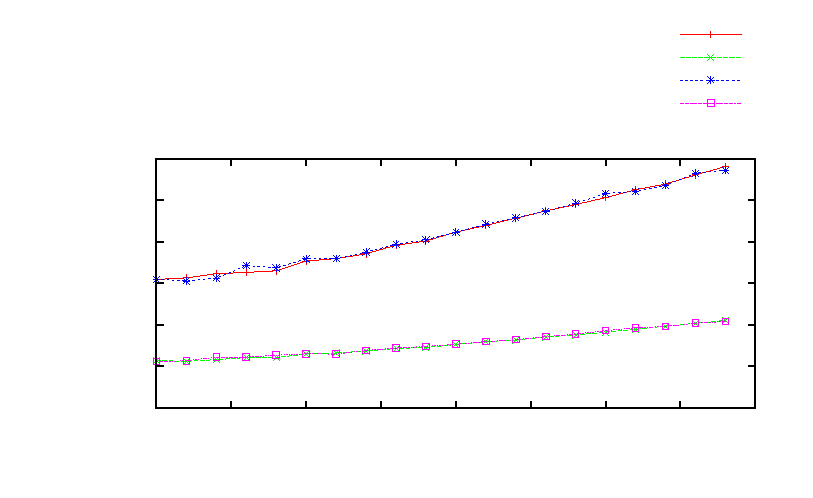
\includegraphics{L2L3NaiveVsControlledNodeMemorySkewRankQueryCacheMisses}}%
    \gplfronttext
  \end{picture}%
\endgroup

	\caption{Level 2 Data and 3 Total Cache Misses}
	\label{fig:L2L3NaiveControlledNodeMemoryRankSkewCacheMisses}
\end{subfigure}

\begin{subfigure}{0.48\textwidth}
	% GNUPLOT: LaTeX picture with Postscript
\begingroup
  \makeatletter
  \providecommand\color[2][]{%
    \GenericError{(gnuplot) \space\space\space\@spaces}{%
      Package color not loaded in conjunction with
      terminal option `colourtext'%
    }{See the gnuplot documentation for explanation.%
    }{Either use 'blacktext' in gnuplot or load the package
      color.sty in LaTeX.}%
    \renewcommand\color[2][]{}%
  }%
  \providecommand\includegraphics[2][]{%
    \GenericError{(gnuplot) \space\space\space\@spaces}{%
      Package graphicx or graphics not loaded%
    }{See the gnuplot documentation for explanation.%
    }{The gnuplot epslatex terminal needs graphicx.sty or graphics.sty.}%
    \renewcommand\includegraphics[2][]{}%
  }%
  \providecommand\rotatebox[2]{#2}%
  \@ifundefined{ifGPcolor}{%
    \newif\ifGPcolor
    \GPcolortrue
  }{}%
  \@ifundefined{ifGPblacktext}{%
    \newif\ifGPblacktext
    \GPblacktexttrue
  }{}%
  % define a \g@addto@macro without @ in the name:
  \let\gplgaddtomacro\g@addto@macro
  % define empty templates for all commands taking text:
  \gdef\gplbacktext{}%
  \gdef\gplfronttext{}%
  \makeatother
  \ifGPblacktext
    % no textcolor at all
    \def\colorrgb#1{}%
    \def\colorgray#1{}%
  \else
    % gray or color?
    \ifGPcolor
      \def\colorrgb#1{\color[rgb]{#1}}%
      \def\colorgray#1{\color[gray]{#1}}%
      \expandafter\def\csname LTw\endcsname{\color{white}}%
      \expandafter\def\csname LTb\endcsname{\color{black}}%
      \expandafter\def\csname LTa\endcsname{\color{black}}%
      \expandafter\def\csname LT0\endcsname{\color[rgb]{1,0,0}}%
      \expandafter\def\csname LT1\endcsname{\color[rgb]{0,1,0}}%
      \expandafter\def\csname LT2\endcsname{\color[rgb]{0,0,1}}%
      \expandafter\def\csname LT3\endcsname{\color[rgb]{1,0,1}}%
      \expandafter\def\csname LT4\endcsname{\color[rgb]{0,1,1}}%
      \expandafter\def\csname LT5\endcsname{\color[rgb]{1,1,0}}%
      \expandafter\def\csname LT6\endcsname{\color[rgb]{0,0,0}}%
      \expandafter\def\csname LT7\endcsname{\color[rgb]{1,0.3,0}}%
      \expandafter\def\csname LT8\endcsname{\color[rgb]{0.5,0.5,0.5}}%
    \else
      % gray
      \def\colorrgb#1{\color{black}}%
      \def\colorgray#1{\color[gray]{#1}}%
      \expandafter\def\csname LTw\endcsname{\color{white}}%
      \expandafter\def\csname LTb\endcsname{\color{black}}%
      \expandafter\def\csname LTa\endcsname{\color{black}}%
      \expandafter\def\csname LT0\endcsname{\color{black}}%
      \expandafter\def\csname LT1\endcsname{\color{black}}%
      \expandafter\def\csname LT2\endcsname{\color{black}}%
      \expandafter\def\csname LT3\endcsname{\color{black}}%
      \expandafter\def\csname LT4\endcsname{\color{black}}%
      \expandafter\def\csname LT5\endcsname{\color{black}}%
      \expandafter\def\csname LT6\endcsname{\color{black}}%
      \expandafter\def\csname LT7\endcsname{\color{black}}%
      \expandafter\def\csname LT8\endcsname{\color{black}}%
    \fi
  \fi
  \setlength{\unitlength}{0.0500bp}%
  \begin{picture}(7488.00,4464.00)%
    \gplgaddtomacro\gplbacktext{%
      \csname LTb\endcsname%
      \put(1078,704){\makebox(0,0)[r]{\strut{} 0}}%
      \put(1078,1058){\makebox(0,0)[r]{\strut{} 0.01}}%
      \put(1078,1413){\makebox(0,0)[r]{\strut{} 0.02}}%
      \put(1078,1767){\makebox(0,0)[r]{\strut{} 0.03}}%
      \put(1078,2122){\makebox(0,0)[r]{\strut{} 0.04}}%
      \put(1078,2476){\makebox(0,0)[r]{\strut{} 0.05}}%
      \put(1078,2830){\makebox(0,0)[r]{\strut{} 0.06}}%
      \put(1078,3185){\makebox(0,0)[r]{\strut{} 0.07}}%
      \put(1078,3539){\makebox(0,0)[r]{\strut{} 0.08}}%
      \put(1210,484){\makebox(0,0){\strut{} 2}}%
      \put(1945,484){\makebox(0,0){\strut{} 2.5}}%
      \put(2680,484){\makebox(0,0){\strut{} 3}}%
      \put(3415,484){\makebox(0,0){\strut{} 3.5}}%
      \put(4151,484){\makebox(0,0){\strut{} 4}}%
      \put(4886,484){\makebox(0,0){\strut{} 4.5}}%
      \put(5621,484){\makebox(0,0){\strut{} 5}}%
      \put(6356,484){\makebox(0,0){\strut{} 5.5}}%
      \put(7091,484){\makebox(0,0){\strut{} 6}}%
      \put(176,2121){\rotatebox{-270}{\makebox(0,0){\strut{}L2 Cache miss rate}}}%
      \put(4150,154){\makebox(0,0){\strut{}Skew}}%
    }%
    \gplgaddtomacro\gplfronttext{%
      \csname LTb\endcsname%
      \put(6236,4291){\makebox(0,0)[r]{\strut{}Naive $mr\hat{\sigma}=$14.395 $avg\hat{\sigma}=$4.57}}%
      \csname LTb\endcsname%
      \put(6236,4071){\makebox(0,0)[r]{\strut{}ControlledNodeMemory $mr\hat{\sigma}=$55.041 $avg\hat{\sigma}=$20.23}}%
    }%
    \gplbacktext
    \put(0,0){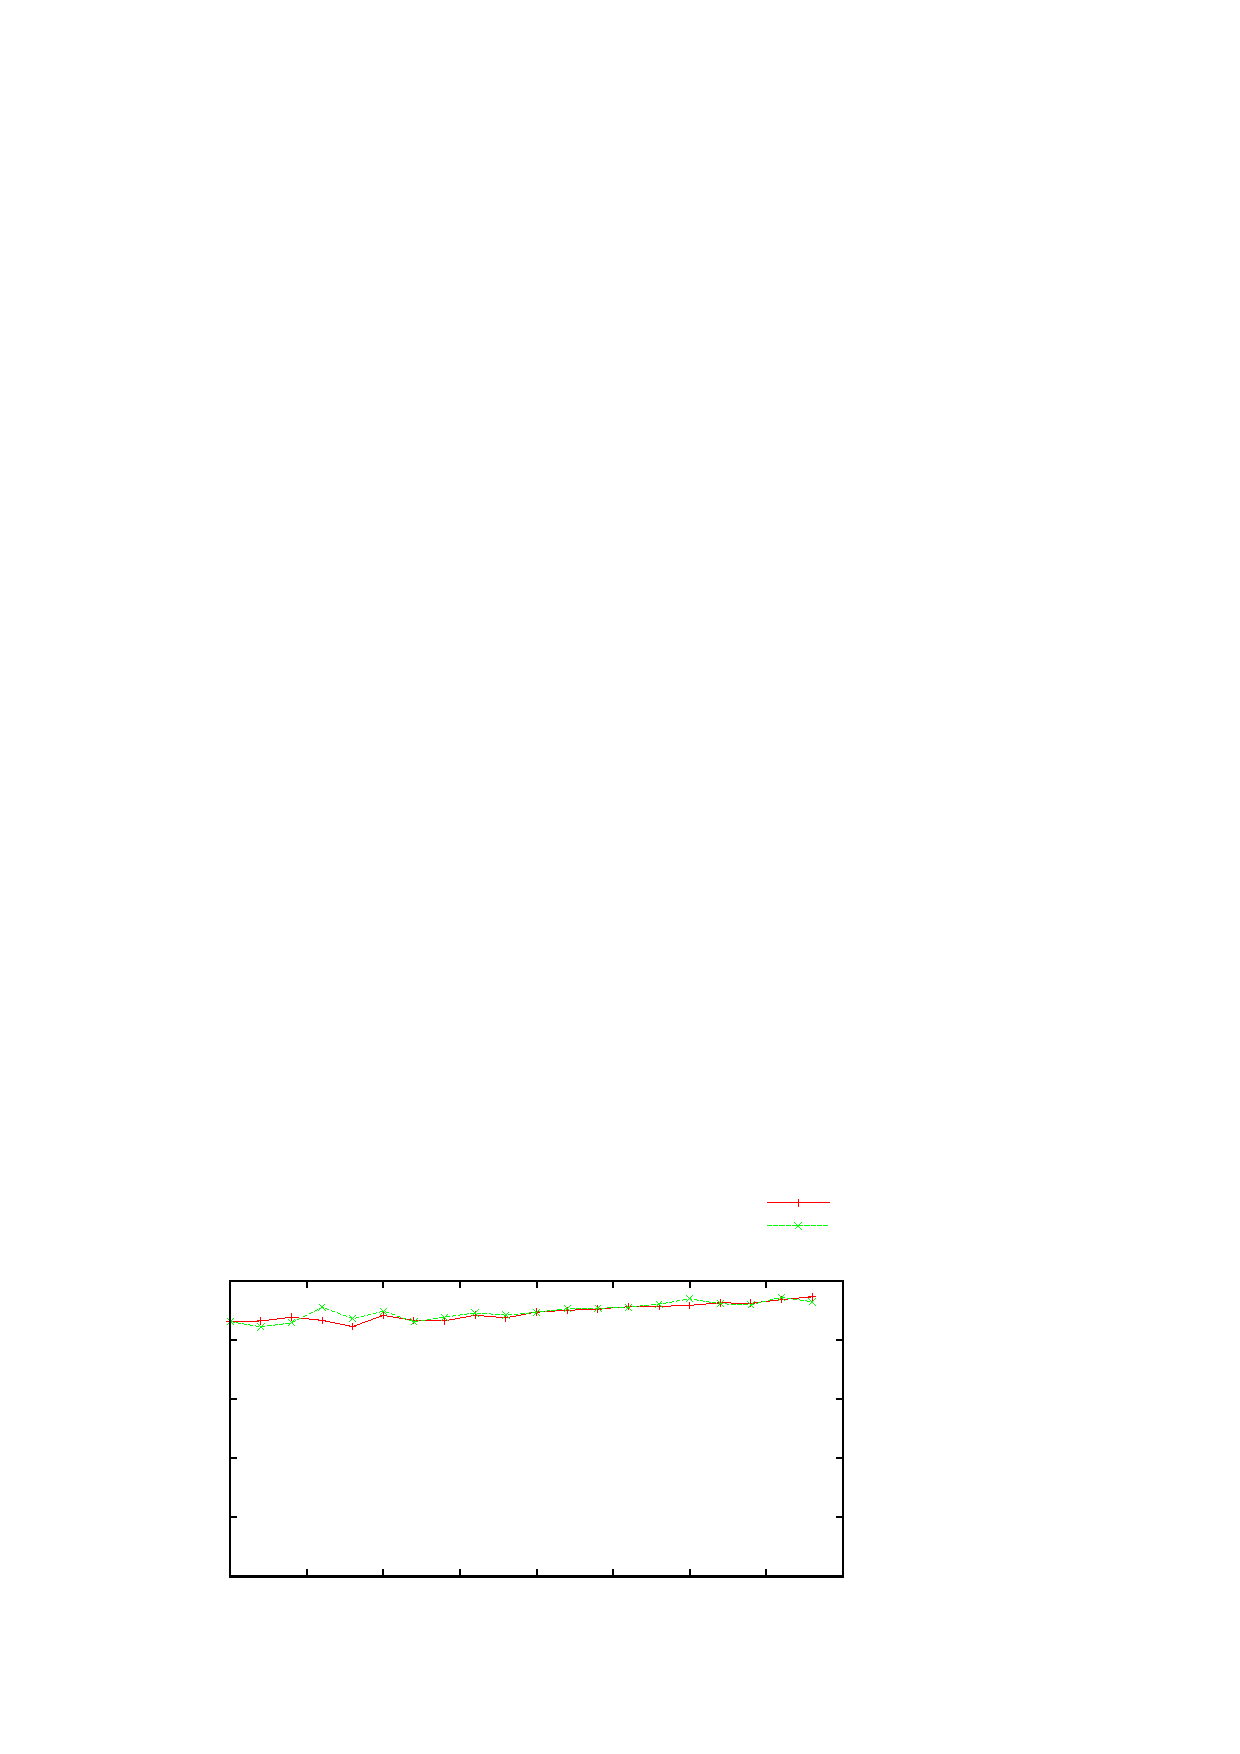
\includegraphics{NaiveVsControlledNodeMemorySkewRankQuery_L2_DCMrate}}%
    \gplfronttext
  \end{picture}%
\endgroup

	\caption{Level 2 Data Cache Miss Rate}
	\label{fig:NaiveVsControlledNodeMemorySkewRankQuery_L2_DCMrate}
\end{subfigure}
\hfill
\begin{subfigure}{0.48\textwidth}
	% GNUPLOT: LaTeX picture with Postscript
\begingroup
  \makeatletter
  \providecommand\color[2][]{%
    \GenericError{(gnuplot) \space\space\space\@spaces}{%
      Package color not loaded in conjunction with
      terminal option `colourtext'%
    }{See the gnuplot documentation for explanation.%
    }{Either use 'blacktext' in gnuplot or load the package
      color.sty in LaTeX.}%
    \renewcommand\color[2][]{}%
  }%
  \providecommand\includegraphics[2][]{%
    \GenericError{(gnuplot) \space\space\space\@spaces}{%
      Package graphicx or graphics not loaded%
    }{See the gnuplot documentation for explanation.%
    }{The gnuplot epslatex terminal needs graphicx.sty or graphics.sty.}%
    \renewcommand\includegraphics[2][]{}%
  }%
  \providecommand\rotatebox[2]{#2}%
  \@ifundefined{ifGPcolor}{%
    \newif\ifGPcolor
    \GPcolortrue
  }{}%
  \@ifundefined{ifGPblacktext}{%
    \newif\ifGPblacktext
    \GPblacktexttrue
  }{}%
  % define a \g@addto@macro without @ in the name:
  \let\gplgaddtomacro\g@addto@macro
  % define empty templates for all commands taking text:
  \gdef\gplbacktext{}%
  \gdef\gplfronttext{}%
  \makeatother
  \ifGPblacktext
    % no textcolor at all
    \def\colorrgb#1{}%
    \def\colorgray#1{}%
  \else
    % gray or color?
    \ifGPcolor
      \def\colorrgb#1{\color[rgb]{#1}}%
      \def\colorgray#1{\color[gray]{#1}}%
      \expandafter\def\csname LTw\endcsname{\color{white}}%
      \expandafter\def\csname LTb\endcsname{\color{black}}%
      \expandafter\def\csname LTa\endcsname{\color{black}}%
      \expandafter\def\csname LT0\endcsname{\color[rgb]{1,0,0}}%
      \expandafter\def\csname LT1\endcsname{\color[rgb]{0,1,0}}%
      \expandafter\def\csname LT2\endcsname{\color[rgb]{0,0,1}}%
      \expandafter\def\csname LT3\endcsname{\color[rgb]{1,0,1}}%
      \expandafter\def\csname LT4\endcsname{\color[rgb]{0,1,1}}%
      \expandafter\def\csname LT5\endcsname{\color[rgb]{1,1,0}}%
      \expandafter\def\csname LT6\endcsname{\color[rgb]{0,0,0}}%
      \expandafter\def\csname LT7\endcsname{\color[rgb]{1,0.3,0}}%
      \expandafter\def\csname LT8\endcsname{\color[rgb]{0.5,0.5,0.5}}%
    \else
      % gray
      \def\colorrgb#1{\color{black}}%
      \def\colorgray#1{\color[gray]{#1}}%
      \expandafter\def\csname LTw\endcsname{\color{white}}%
      \expandafter\def\csname LTb\endcsname{\color{black}}%
      \expandafter\def\csname LTa\endcsname{\color{black}}%
      \expandafter\def\csname LT0\endcsname{\color{black}}%
      \expandafter\def\csname LT1\endcsname{\color{black}}%
      \expandafter\def\csname LT2\endcsname{\color{black}}%
      \expandafter\def\csname LT3\endcsname{\color{black}}%
      \expandafter\def\csname LT4\endcsname{\color{black}}%
      \expandafter\def\csname LT5\endcsname{\color{black}}%
      \expandafter\def\csname LT6\endcsname{\color{black}}%
      \expandafter\def\csname LT7\endcsname{\color{black}}%
      \expandafter\def\csname LT8\endcsname{\color{black}}%
    \fi
  \fi
  \setlength{\unitlength}{0.0500bp}%
  \begin{picture}(4608.00,3600.00)%
    \gplgaddtomacro\gplbacktext{%
      \csname LTb\endcsname%
      \put(804,384){\makebox(0,0)[r]{\strut{} 0}}%
      \put(804,823){\makebox(0,0)[r]{\strut{} 200000}}%
      \put(804,1261){\makebox(0,0)[r]{\strut{} 400000}}%
      \put(804,1700){\makebox(0,0)[r]{\strut{} 600000}}%
      \put(804,2139){\makebox(0,0)[r]{\strut{} 800000}}%
      \put(804,2578){\makebox(0,0)[r]{\strut{} 1e+06}}%
      \put(804,3016){\makebox(0,0)[r]{\strut{} 1.2e+06}}%
      \put(804,3455){\makebox(0,0)[r]{\strut{} 1.4e+06}}%
      \put(876,264){\makebox(0,0){\strut{} 2}}%
      \put(1315,264){\makebox(0,0){\strut{} 2.5}}%
      \put(1755,264){\makebox(0,0){\strut{} 3}}%
      \put(2194,264){\makebox(0,0){\strut{} 3.5}}%
      \put(2634,264){\makebox(0,0){\strut{} 4}}%
      \put(3073,264){\makebox(0,0){\strut{} 4.5}}%
      \put(3512,264){\makebox(0,0){\strut{} 5}}%
      \put(3952,264){\makebox(0,0){\strut{} 5.5}}%
      \put(4391,264){\makebox(0,0){\strut{} 6}}%
      \put(96,1919){\rotatebox{-270}{\makebox(0,0){\strut{}TLB}}}%
      \put(2633,84){\makebox(0,0){\strut{}Skew}}%
    }%
    \gplgaddtomacro\gplfronttext{%
      \csname LTb\endcsname%
      \put(1889,3332){\makebox(0,0)[r]{\strut{}Naive}}%
      \csname LTb\endcsname%
      \put(3824,3332){\makebox(0,0)[r]{\strut{}ControlledNodeMemory}}%
    }%
    \gplbacktext
    \put(0,0){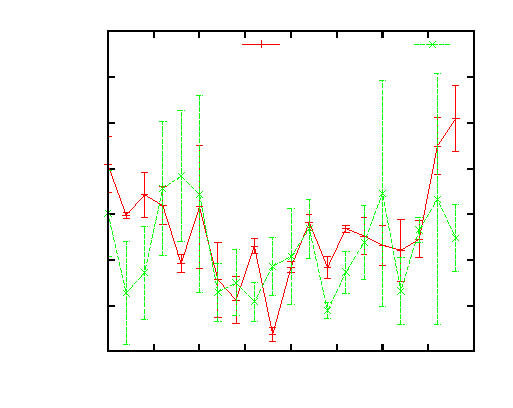
\includegraphics{NaiveVsControlledNodeMemorySkewRankQueryTLB}}%
    \gplfronttext
  \end{picture}%
\endgroup

	\caption{TLB Misses}
	\label{fig:NaiveVsControlledNodeMemorySkewRankQueryTLB}
\end{subfigure}

\caption{Various measurements for Rank queries on SimpleNaive and ControlledMemory wavelet trees with various skew.}
\label{fig:NaiveVsControlledNodeMemorySkewRankQuery}

\end{figure}



\begin{figure}\tiny
\begin{subfigure}{0.48\textwidth}
	% GNUPLOT: LaTeX picture with Postscript
\begingroup
  \makeatletter
  \providecommand\color[2][]{%
    \GenericError{(gnuplot) \space\space\space\@spaces}{%
      Package color not loaded in conjunction with
      terminal option `colourtext'%
    }{See the gnuplot documentation for explanation.%
    }{Either use 'blacktext' in gnuplot or load the package
      color.sty in LaTeX.}%
    \renewcommand\color[2][]{}%
  }%
  \providecommand\includegraphics[2][]{%
    \GenericError{(gnuplot) \space\space\space\@spaces}{%
      Package graphicx or graphics not loaded%
    }{See the gnuplot documentation for explanation.%
    }{The gnuplot epslatex terminal needs graphicx.sty or graphics.sty.}%
    \renewcommand\includegraphics[2][]{}%
  }%
  \providecommand\rotatebox[2]{#2}%
  \@ifundefined{ifGPcolor}{%
    \newif\ifGPcolor
    \GPcolortrue
  }{}%
  \@ifundefined{ifGPblacktext}{%
    \newif\ifGPblacktext
    \GPblacktexttrue
  }{}%
  % define a \g@addto@macro without @ in the name:
  \let\gplgaddtomacro\g@addto@macro
  % define empty templates for all commands taking text:
  \gdef\gplbacktext{}%
  \gdef\gplfronttext{}%
  \makeatother
  \ifGPblacktext
    % no textcolor at all
    \def\colorrgb#1{}%
    \def\colorgray#1{}%
  \else
    % gray or color?
    \ifGPcolor
      \def\colorrgb#1{\color[rgb]{#1}}%
      \def\colorgray#1{\color[gray]{#1}}%
      \expandafter\def\csname LTw\endcsname{\color{white}}%
      \expandafter\def\csname LTb\endcsname{\color{black}}%
      \expandafter\def\csname LTa\endcsname{\color{black}}%
      \expandafter\def\csname LT0\endcsname{\color[rgb]{1,0,0}}%
      \expandafter\def\csname LT1\endcsname{\color[rgb]{0,1,0}}%
      \expandafter\def\csname LT2\endcsname{\color[rgb]{0,0,1}}%
      \expandafter\def\csname LT3\endcsname{\color[rgb]{1,0,1}}%
      \expandafter\def\csname LT4\endcsname{\color[rgb]{0,1,1}}%
      \expandafter\def\csname LT5\endcsname{\color[rgb]{1,1,0}}%
      \expandafter\def\csname LT6\endcsname{\color[rgb]{0,0,0}}%
      \expandafter\def\csname LT7\endcsname{\color[rgb]{1,0.3,0}}%
      \expandafter\def\csname LT8\endcsname{\color[rgb]{0.5,0.5,0.5}}%
    \else
      % gray
      \def\colorrgb#1{\color{black}}%
      \def\colorgray#1{\color[gray]{#1}}%
      \expandafter\def\csname LTw\endcsname{\color{white}}%
      \expandafter\def\csname LTb\endcsname{\color{black}}%
      \expandafter\def\csname LTa\endcsname{\color{black}}%
      \expandafter\def\csname LT0\endcsname{\color{black}}%
      \expandafter\def\csname LT1\endcsname{\color{black}}%
      \expandafter\def\csname LT2\endcsname{\color{black}}%
      \expandafter\def\csname LT3\endcsname{\color{black}}%
      \expandafter\def\csname LT4\endcsname{\color{black}}%
      \expandafter\def\csname LT5\endcsname{\color{black}}%
      \expandafter\def\csname LT6\endcsname{\color{black}}%
      \expandafter\def\csname LT7\endcsname{\color{black}}%
      \expandafter\def\csname LT8\endcsname{\color{black}}%
    \fi
  \fi
  \setlength{\unitlength}{0.0500bp}%
  \begin{picture}(4608.00,3600.00)%
    \gplgaddtomacro\gplbacktext{%
      \csname LTb\endcsname%
      \put(516,384){\makebox(0,0)[r]{\strut{} 0}}%
      \put(516,896){\makebox(0,0)[r]{\strut{} 0.5}}%
      \put(516,1408){\makebox(0,0)[r]{\strut{} 1}}%
      \put(516,1920){\makebox(0,0)[r]{\strut{} 1.5}}%
      \put(516,2431){\makebox(0,0)[r]{\strut{} 2}}%
      \put(516,2943){\makebox(0,0)[r]{\strut{} 2.5}}%
      \put(516,3455){\makebox(0,0)[r]{\strut{} 3}}%
      \put(588,264){\makebox(0,0){\strut{} 2}}%
      \put(1063,264){\makebox(0,0){\strut{} 2.5}}%
      \put(1539,264){\makebox(0,0){\strut{} 3}}%
      \put(2014,264){\makebox(0,0){\strut{} 3.5}}%
      \put(2490,264){\makebox(0,0){\strut{} 4}}%
      \put(2965,264){\makebox(0,0){\strut{} 4.5}}%
      \put(3440,264){\makebox(0,0){\strut{} 5}}%
      \put(3916,264){\makebox(0,0){\strut{} 5.5}}%
      \put(4391,264){\makebox(0,0){\strut{} 6}}%
      \put(96,1919){\rotatebox{-270}{\makebox(0,0){\strut{}Wall Time (sec)}}}%
      \put(2489,84){\makebox(0,0){\strut{}Skew}}%
    }%
    \gplgaddtomacro\gplfronttext{%
      \csname LTb\endcsname%
      \put(1812,3332){\makebox(0,0)[r]{\strut{}NaiveInteger}}%
      \csname LTb\endcsname%
      \put(3459,3332){\makebox(0,0)[r]{\strut{}ControlledMemory}}%
    }%
    \gplbacktext
    \put(0,0){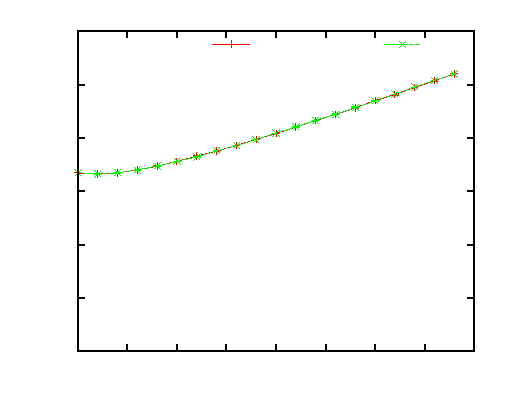
\includegraphics{naiveSelectSkewRunningTime}}%
    \gplfronttext
  \end{picture}%
\endgroup

	\caption{Wall Time}
	\label{fig:NaiveSelectSkewRunningTime}
\end{subfigure}
\hfill
\begin{subfigure}{0.48\textwidth}
	% GNUPLOT: LaTeX picture with Postscript
\begingroup
  \makeatletter
  \providecommand\color[2][]{%
    \GenericError{(gnuplot) \space\space\space\@spaces}{%
      Package color not loaded in conjunction with
      terminal option `colourtext'%
    }{See the gnuplot documentation for explanation.%
    }{Either use 'blacktext' in gnuplot or load the package
      color.sty in LaTeX.}%
    \renewcommand\color[2][]{}%
  }%
  \providecommand\includegraphics[2][]{%
    \GenericError{(gnuplot) \space\space\space\@spaces}{%
      Package graphicx or graphics not loaded%
    }{See the gnuplot documentation for explanation.%
    }{The gnuplot epslatex terminal needs graphicx.sty or graphics.sty.}%
    \renewcommand\includegraphics[2][]{}%
  }%
  \providecommand\rotatebox[2]{#2}%
  \@ifundefined{ifGPcolor}{%
    \newif\ifGPcolor
    \GPcolortrue
  }{}%
  \@ifundefined{ifGPblacktext}{%
    \newif\ifGPblacktext
    \GPblacktexttrue
  }{}%
  % define a \g@addto@macro without @ in the name:
  \let\gplgaddtomacro\g@addto@macro
  % define empty templates for all commands taking text:
  \gdef\gplbacktext{}%
  \gdef\gplfronttext{}%
  \makeatother
  \ifGPblacktext
    % no textcolor at all
    \def\colorrgb#1{}%
    \def\colorgray#1{}%
  \else
    % gray or color?
    \ifGPcolor
      \def\colorrgb#1{\color[rgb]{#1}}%
      \def\colorgray#1{\color[gray]{#1}}%
      \expandafter\def\csname LTw\endcsname{\color{white}}%
      \expandafter\def\csname LTb\endcsname{\color{black}}%
      \expandafter\def\csname LTa\endcsname{\color{black}}%
      \expandafter\def\csname LT0\endcsname{\color[rgb]{1,0,0}}%
      \expandafter\def\csname LT1\endcsname{\color[rgb]{0,1,0}}%
      \expandafter\def\csname LT2\endcsname{\color[rgb]{0,0,1}}%
      \expandafter\def\csname LT3\endcsname{\color[rgb]{1,0,1}}%
      \expandafter\def\csname LT4\endcsname{\color[rgb]{0,1,1}}%
      \expandafter\def\csname LT5\endcsname{\color[rgb]{1,1,0}}%
      \expandafter\def\csname LT6\endcsname{\color[rgb]{0,0,0}}%
      \expandafter\def\csname LT7\endcsname{\color[rgb]{1,0.3,0}}%
      \expandafter\def\csname LT8\endcsname{\color[rgb]{0.5,0.5,0.5}}%
    \else
      % gray
      \def\colorrgb#1{\color{black}}%
      \def\colorgray#1{\color[gray]{#1}}%
      \expandafter\def\csname LTw\endcsname{\color{white}}%
      \expandafter\def\csname LTb\endcsname{\color{black}}%
      \expandafter\def\csname LTa\endcsname{\color{black}}%
      \expandafter\def\csname LT0\endcsname{\color{black}}%
      \expandafter\def\csname LT1\endcsname{\color{black}}%
      \expandafter\def\csname LT2\endcsname{\color{black}}%
      \expandafter\def\csname LT3\endcsname{\color{black}}%
      \expandafter\def\csname LT4\endcsname{\color{black}}%
      \expandafter\def\csname LT5\endcsname{\color{black}}%
      \expandafter\def\csname LT6\endcsname{\color{black}}%
      \expandafter\def\csname LT7\endcsname{\color{black}}%
      \expandafter\def\csname LT8\endcsname{\color{black}}%
    \fi
  \fi
  \setlength{\unitlength}{0.0500bp}%
  \begin{picture}(7488.00,4752.00)%
    \gplgaddtomacro\gplbacktext{%
      \csname LTb\endcsname%
      \put(1210,704){\makebox(0,0)[r]{\strut{} 0}}%
      \put(1210,1329){\makebox(0,0)[r]{\strut{} 0.005}}%
      \put(1210,1953){\makebox(0,0)[r]{\strut{} 0.01}}%
      \put(1210,2578){\makebox(0,0)[r]{\strut{} 0.015}}%
      \put(1210,3202){\makebox(0,0)[r]{\strut{} 0.02}}%
      \put(1210,3827){\makebox(0,0)[r]{\strut{} 0.025}}%
      \put(1342,484){\makebox(0,0){\strut{} 2}}%
      \put(2061,484){\makebox(0,0){\strut{} 2.5}}%
      \put(2779,484){\makebox(0,0){\strut{} 3}}%
      \put(3498,484){\makebox(0,0){\strut{} 3.5}}%
      \put(4217,484){\makebox(0,0){\strut{} 4}}%
      \put(4935,484){\makebox(0,0){\strut{} 4.5}}%
      \put(5654,484){\makebox(0,0){\strut{} 5}}%
      \put(6372,484){\makebox(0,0){\strut{} 5.5}}%
      \put(7091,484){\makebox(0,0){\strut{} 6}}%
      \put(176,2265){\rotatebox{-270}{\makebox(0,0){\strut{}Branch Misprediction Rate}}}%
      \put(4216,154){\makebox(0,0){\strut{}Skew}}%
    }%
    \gplgaddtomacro\gplfronttext{%
      \csname LTb\endcsname%
      \put(6236,4579){\makebox(0,0)[r]{\strut{}Naive $mr\hat{\sigma}=$0.136 $avg\hat{\sigma}=$0.09}}%
      \csname LTb\endcsname%
      \put(6236,4359){\makebox(0,0)[r]{\strut{}ControlledNodeMemory $mr\hat{\sigma}=$0.789 $avg\hat{\sigma}=$0.17}}%
    }%
    \gplbacktext
    \put(0,0){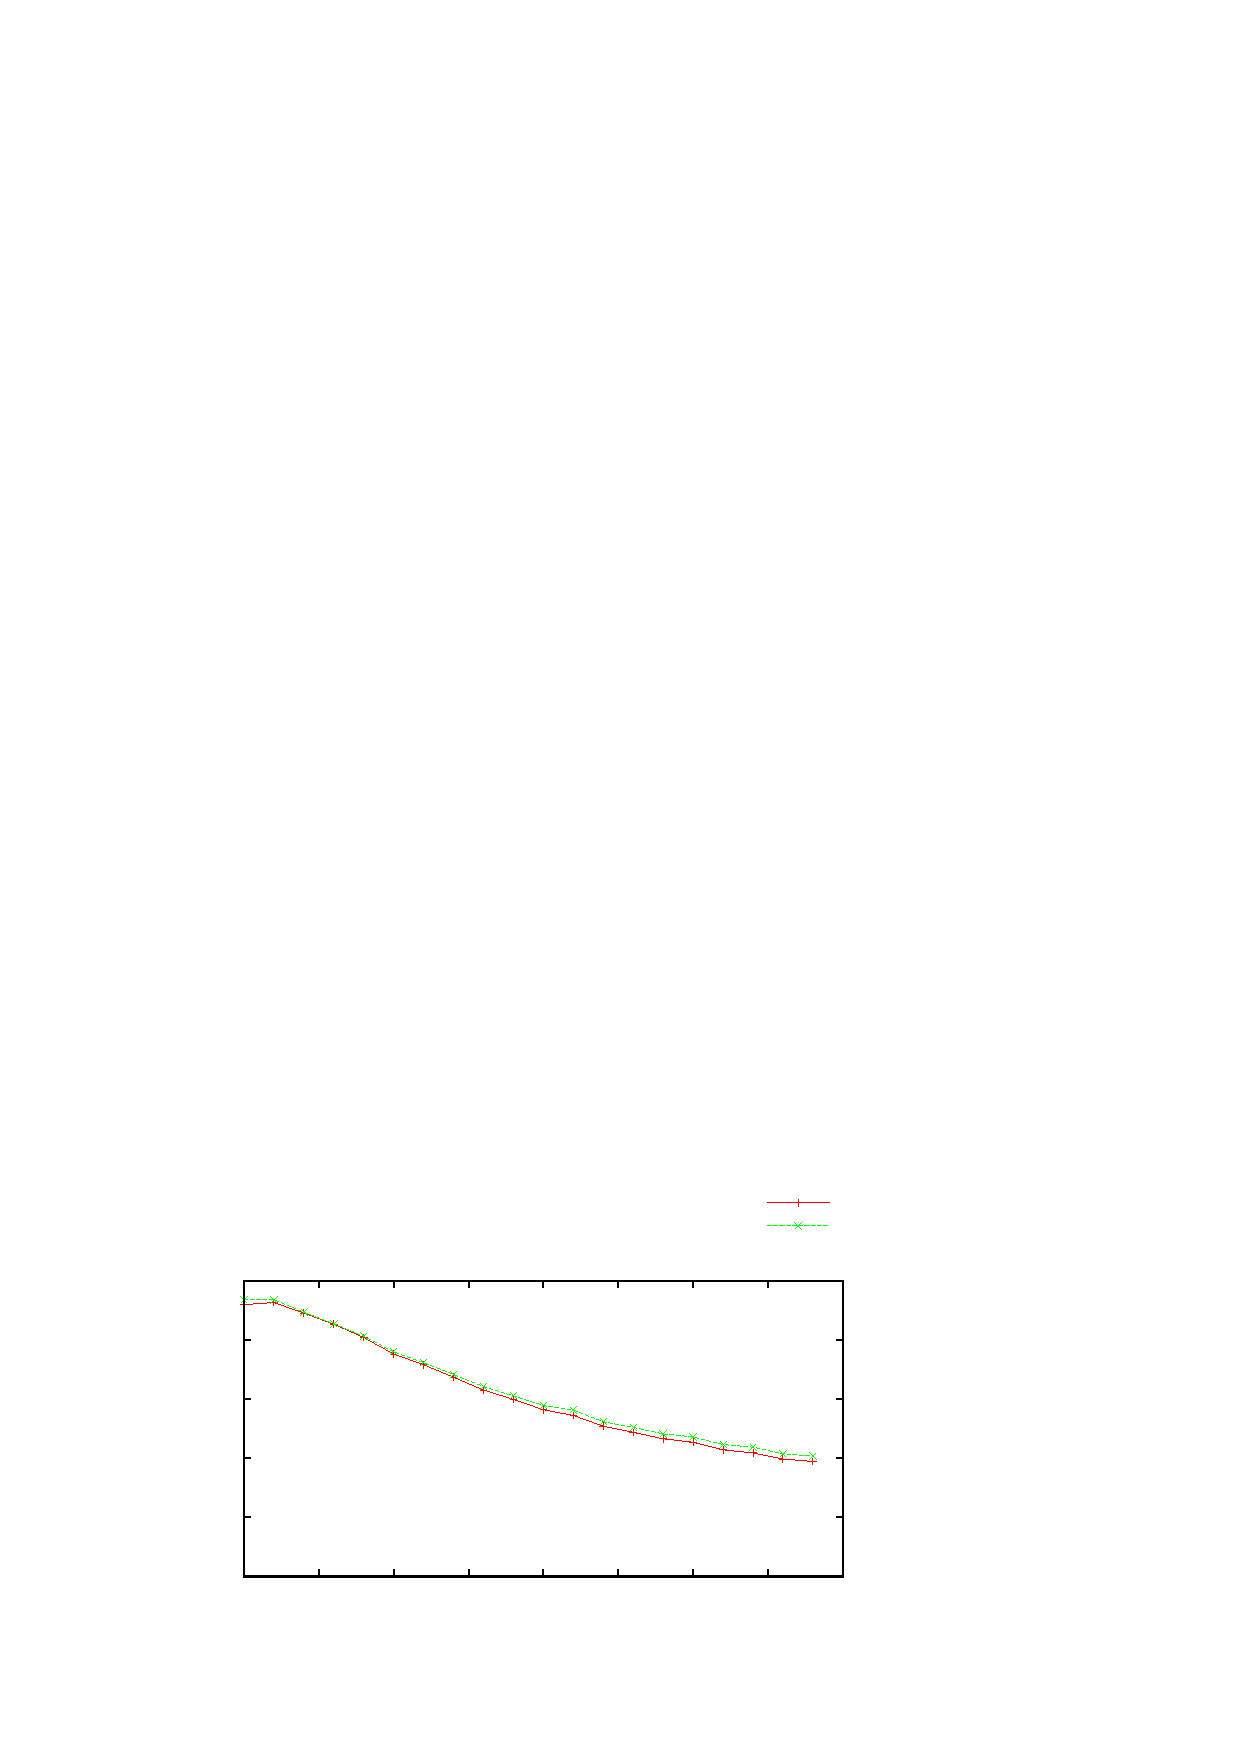
\includegraphics{NaiveVsControlledNodeMemorySkewSelectQuery_BMrate}}%
    \gplfronttext
  \end{picture}%
\endgroup

	\caption{Branch Misprediction Rate}
	\label{fig:NaiveVsControlledNodeMemorySkewSelectQueryBMrate}
\end{subfigure}

\begin{subfigure}{0.48\textwidth}
	% GNUPLOT: LaTeX picture with Postscript
\begingroup
  \makeatletter
  \providecommand\color[2][]{%
    \GenericError{(gnuplot) \space\space\space\@spaces}{%
      Package color not loaded in conjunction with
      terminal option `colourtext'%
    }{See the gnuplot documentation for explanation.%
    }{Either use 'blacktext' in gnuplot or load the package
      color.sty in LaTeX.}%
    \renewcommand\color[2][]{}%
  }%
  \providecommand\includegraphics[2][]{%
    \GenericError{(gnuplot) \space\space\space\@spaces}{%
      Package graphicx or graphics not loaded%
    }{See the gnuplot documentation for explanation.%
    }{The gnuplot epslatex terminal needs graphicx.sty or graphics.sty.}%
    \renewcommand\includegraphics[2][]{}%
  }%
  \providecommand\rotatebox[2]{#2}%
  \@ifundefined{ifGPcolor}{%
    \newif\ifGPcolor
    \GPcolortrue
  }{}%
  \@ifundefined{ifGPblacktext}{%
    \newif\ifGPblacktext
    \GPblacktexttrue
  }{}%
  % define a \g@addto@macro without @ in the name:
  \let\gplgaddtomacro\g@addto@macro
  % define empty templates for all commands taking text:
  \gdef\gplbacktext{}%
  \gdef\gplfronttext{}%
  \makeatother
  \ifGPblacktext
    % no textcolor at all
    \def\colorrgb#1{}%
    \def\colorgray#1{}%
  \else
    % gray or color?
    \ifGPcolor
      \def\colorrgb#1{\color[rgb]{#1}}%
      \def\colorgray#1{\color[gray]{#1}}%
      \expandafter\def\csname LTw\endcsname{\color{white}}%
      \expandafter\def\csname LTb\endcsname{\color{black}}%
      \expandafter\def\csname LTa\endcsname{\color{black}}%
      \expandafter\def\csname LT0\endcsname{\color[rgb]{1,0,0}}%
      \expandafter\def\csname LT1\endcsname{\color[rgb]{0,1,0}}%
      \expandafter\def\csname LT2\endcsname{\color[rgb]{0,0,1}}%
      \expandafter\def\csname LT3\endcsname{\color[rgb]{1,0,1}}%
      \expandafter\def\csname LT4\endcsname{\color[rgb]{0,1,1}}%
      \expandafter\def\csname LT5\endcsname{\color[rgb]{1,1,0}}%
      \expandafter\def\csname LT6\endcsname{\color[rgb]{0,0,0}}%
      \expandafter\def\csname LT7\endcsname{\color[rgb]{1,0.3,0}}%
      \expandafter\def\csname LT8\endcsname{\color[rgb]{0.5,0.5,0.5}}%
    \else
      % gray
      \def\colorrgb#1{\color{black}}%
      \def\colorgray#1{\color[gray]{#1}}%
      \expandafter\def\csname LTw\endcsname{\color{white}}%
      \expandafter\def\csname LTb\endcsname{\color{black}}%
      \expandafter\def\csname LTa\endcsname{\color{black}}%
      \expandafter\def\csname LT0\endcsname{\color{black}}%
      \expandafter\def\csname LT1\endcsname{\color{black}}%
      \expandafter\def\csname LT2\endcsname{\color{black}}%
      \expandafter\def\csname LT3\endcsname{\color{black}}%
      \expandafter\def\csname LT4\endcsname{\color{black}}%
      \expandafter\def\csname LT5\endcsname{\color{black}}%
      \expandafter\def\csname LT6\endcsname{\color{black}}%
      \expandafter\def\csname LT7\endcsname{\color{black}}%
      \expandafter\def\csname LT8\endcsname{\color{black}}%
    \fi
  \fi
  \setlength{\unitlength}{0.0500bp}%
  \begin{picture}(8062.00,4752.00)%
    \gplgaddtomacro\gplbacktext{%
      \csname LTb\endcsname%
      \put(1474,704){\makebox(0,0)[r]{\strut{} 0}}%
      \put(1474,1244){\makebox(0,0)[r]{\strut{} 200000}}%
      \put(1474,1785){\makebox(0,0)[r]{\strut{} 400000}}%
      \put(1474,2325){\makebox(0,0)[r]{\strut{} 600000}}%
      \put(1474,2866){\makebox(0,0)[r]{\strut{} 800000}}%
      \put(1474,3406){\makebox(0,0)[r]{\strut{} 1e+06}}%
      \put(1474,3947){\makebox(0,0)[r]{\strut{} 1.2e+06}}%
      \put(1474,4487){\makebox(0,0)[r]{\strut{} 1.4e+06}}%
      \put(1606,484){\makebox(0,0){\strut{} 2}}%
      \put(2363,484){\makebox(0,0){\strut{} 2.5}}%
      \put(3121,484){\makebox(0,0){\strut{} 3}}%
      \put(3878,484){\makebox(0,0){\strut{} 3.5}}%
      \put(4636,484){\makebox(0,0){\strut{} 4}}%
      \put(5393,484){\makebox(0,0){\strut{} 4.5}}%
      \put(6150,484){\makebox(0,0){\strut{} 5}}%
      \put(6908,484){\makebox(0,0){\strut{} 5.5}}%
      \put(7665,484){\makebox(0,0){\strut{} 6}}%
      \put(176,2595){\rotatebox{-270}{\makebox(0,0){\strut{}Cache Misses}}}%
      \put(4635,154){\makebox(0,0){\strut{}Skew}}%
    }%
    \gplgaddtomacro\gplfronttext{%
      \csname LTb\endcsname%
      \put(6678,1097){\makebox(0,0)[r]{\strut{}Naive L1 $mr\sigma=$0.302}}%
      \csname LTb\endcsname%
      \put(6678,877){\makebox(0,0)[r]{\strut{}ControlledNodeMemory L1 $mr\sigma=$2.589}}%
    }%
    \gplbacktext
    \put(0,0){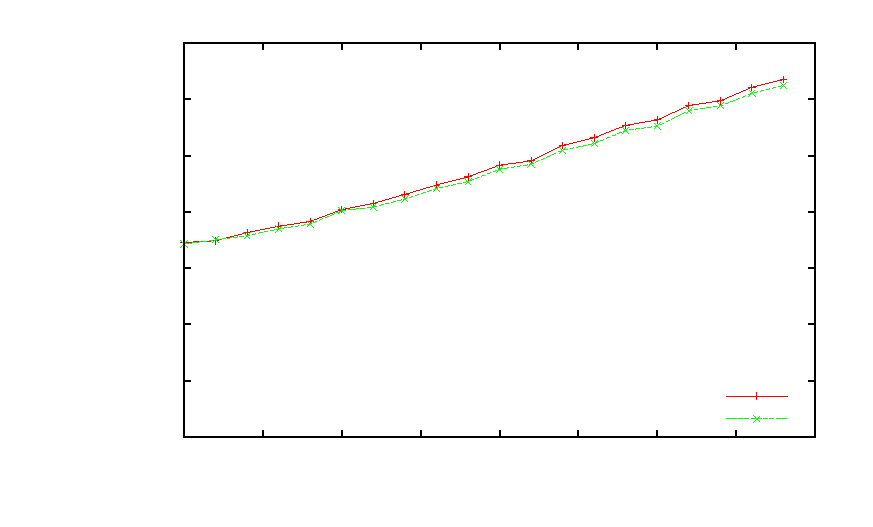
\includegraphics{L1NaiveVsControlledNodeMemorySkewSelectQueryCacheMisses}}%
    \gplfronttext
  \end{picture}%
\endgroup

	\caption{Level 1 Data Cache Misses}
	\label{fig:L1NaiveControlledNodeMemorySelectSkewCacheMisses}
\end{subfigure}
\hfill
\begin{subfigure}{0.48\textwidth}
 	% GNUPLOT: LaTeX picture with Postscript
\begingroup
  \makeatletter
  \providecommand\color[2][]{%
    \GenericError{(gnuplot) \space\space\space\@spaces}{%
      Package color not loaded in conjunction with
      terminal option `colourtext'%
    }{See the gnuplot documentation for explanation.%
    }{Either use 'blacktext' in gnuplot or load the package
      color.sty in LaTeX.}%
    \renewcommand\color[2][]{}%
  }%
  \providecommand\includegraphics[2][]{%
    \GenericError{(gnuplot) \space\space\space\@spaces}{%
      Package graphicx or graphics not loaded%
    }{See the gnuplot documentation for explanation.%
    }{The gnuplot epslatex terminal needs graphicx.sty or graphics.sty.}%
    \renewcommand\includegraphics[2][]{}%
  }%
  \providecommand\rotatebox[2]{#2}%
  \@ifundefined{ifGPcolor}{%
    \newif\ifGPcolor
    \GPcolortrue
  }{}%
  \@ifundefined{ifGPblacktext}{%
    \newif\ifGPblacktext
    \GPblacktexttrue
  }{}%
  % define a \g@addto@macro without @ in the name:
  \let\gplgaddtomacro\g@addto@macro
  % define empty templates for all commands taking text:
  \gdef\gplbacktext{}%
  \gdef\gplfronttext{}%
  \makeatother
  \ifGPblacktext
    % no textcolor at all
    \def\colorrgb#1{}%
    \def\colorgray#1{}%
  \else
    % gray or color?
    \ifGPcolor
      \def\colorrgb#1{\color[rgb]{#1}}%
      \def\colorgray#1{\color[gray]{#1}}%
      \expandafter\def\csname LTw\endcsname{\color{white}}%
      \expandafter\def\csname LTb\endcsname{\color{black}}%
      \expandafter\def\csname LTa\endcsname{\color{black}}%
      \expandafter\def\csname LT0\endcsname{\color[rgb]{1,0,0}}%
      \expandafter\def\csname LT1\endcsname{\color[rgb]{0,1,0}}%
      \expandafter\def\csname LT2\endcsname{\color[rgb]{0,0,1}}%
      \expandafter\def\csname LT3\endcsname{\color[rgb]{1,0,1}}%
      \expandafter\def\csname LT4\endcsname{\color[rgb]{0,1,1}}%
      \expandafter\def\csname LT5\endcsname{\color[rgb]{1,1,0}}%
      \expandafter\def\csname LT6\endcsname{\color[rgb]{0,0,0}}%
      \expandafter\def\csname LT7\endcsname{\color[rgb]{1,0.3,0}}%
      \expandafter\def\csname LT8\endcsname{\color[rgb]{0.5,0.5,0.5}}%
    \else
      % gray
      \def\colorrgb#1{\color{black}}%
      \def\colorgray#1{\color[gray]{#1}}%
      \expandafter\def\csname LTw\endcsname{\color{white}}%
      \expandafter\def\csname LTb\endcsname{\color{black}}%
      \expandafter\def\csname LTa\endcsname{\color{black}}%
      \expandafter\def\csname LT0\endcsname{\color{black}}%
      \expandafter\def\csname LT1\endcsname{\color{black}}%
      \expandafter\def\csname LT2\endcsname{\color{black}}%
      \expandafter\def\csname LT3\endcsname{\color{black}}%
      \expandafter\def\csname LT4\endcsname{\color{black}}%
      \expandafter\def\csname LT5\endcsname{\color{black}}%
      \expandafter\def\csname LT6\endcsname{\color{black}}%
      \expandafter\def\csname LT7\endcsname{\color{black}}%
      \expandafter\def\csname LT8\endcsname{\color{black}}%
    \fi
  \fi
  \setlength{\unitlength}{0.0500bp}%
  \begin{picture}(4608.00,3600.00)%
    \gplgaddtomacro\gplbacktext{%
      \csname LTb\endcsname%
      \put(804,384){\makebox(0,0)[r]{\strut{} 0}}%
      \put(804,768){\makebox(0,0)[r]{\strut{} 2e+06}}%
      \put(804,1152){\makebox(0,0)[r]{\strut{} 4e+06}}%
      \put(804,1536){\makebox(0,0)[r]{\strut{} 6e+06}}%
      \put(804,1920){\makebox(0,0)[r]{\strut{} 8e+06}}%
      \put(804,2303){\makebox(0,0)[r]{\strut{} 1e+07}}%
      \put(804,2687){\makebox(0,0)[r]{\strut{} 1.2e+07}}%
      \put(804,3071){\makebox(0,0)[r]{\strut{} 1.4e+07}}%
      \put(804,3455){\makebox(0,0)[r]{\strut{} 1.6e+07}}%
      \put(876,264){\makebox(0,0){\strut{} 2}}%
      \put(1315,264){\makebox(0,0){\strut{} 2.5}}%
      \put(1755,264){\makebox(0,0){\strut{} 3}}%
      \put(2194,264){\makebox(0,0){\strut{} 3.5}}%
      \put(2634,264){\makebox(0,0){\strut{} 4}}%
      \put(3073,264){\makebox(0,0){\strut{} 4.5}}%
      \put(3512,264){\makebox(0,0){\strut{} 5}}%
      \put(3952,264){\makebox(0,0){\strut{} 5.5}}%
      \put(4391,264){\makebox(0,0){\strut{} 6}}%
      \put(96,1919){\rotatebox{-270}{\makebox(0,0){\strut{}Cache Misses}}}%
      \put(2633,84){\makebox(0,0){\strut{}Skew}}%
    }%
    \gplgaddtomacro\gplfronttext{%
      \csname LTb\endcsname%
      \put(1673,3332){\makebox(0,0)[r]{\strut{}Naive L2}}%
      \csname LTb\endcsname%
      \put(1673,3212){\makebox(0,0)[r]{\strut{}Naive L3}}%
      \csname LTb\endcsname%
      \put(3824,3332){\makebox(0,0)[r]{\strut{}ControlledNodeMemory L2}}%
      \csname LTb\endcsname%
      \put(3824,3212){\makebox(0,0)[r]{\strut{}ControlledNodeMemory L3}}%
    }%
    \gplbacktext
    \put(0,0){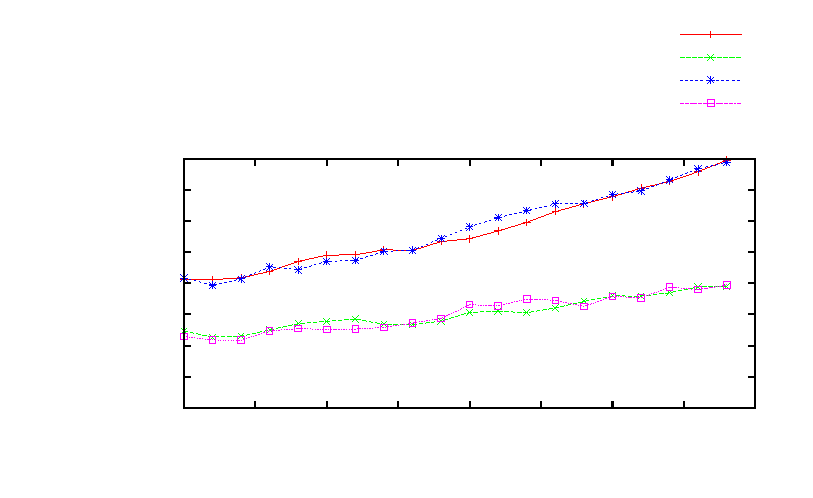
\includegraphics{L2L3NaiveVsControlledNodeMemorySkewSelectQueryCacheMisses}}%
    \gplfronttext
  \end{picture}%
\endgroup

	\caption{Level 2 Data and 3 Total Cache Misses}
	\label{fig:L2L3NaiveControlledNodeMemorySelectSkewCacheMisses}
\end{subfigure}

\begin{subfigure}{0.48\textwidth}
	% GNUPLOT: LaTeX picture with Postscript
\begingroup
  \makeatletter
  \providecommand\color[2][]{%
    \GenericError{(gnuplot) \space\space\space\@spaces}{%
      Package color not loaded in conjunction with
      terminal option `colourtext'%
    }{See the gnuplot documentation for explanation.%
    }{Either use 'blacktext' in gnuplot or load the package
      color.sty in LaTeX.}%
    \renewcommand\color[2][]{}%
  }%
  \providecommand\includegraphics[2][]{%
    \GenericError{(gnuplot) \space\space\space\@spaces}{%
      Package graphicx or graphics not loaded%
    }{See the gnuplot documentation for explanation.%
    }{The gnuplot epslatex terminal needs graphicx.sty or graphics.sty.}%
    \renewcommand\includegraphics[2][]{}%
  }%
  \providecommand\rotatebox[2]{#2}%
  \@ifundefined{ifGPcolor}{%
    \newif\ifGPcolor
    \GPcolortrue
  }{}%
  \@ifundefined{ifGPblacktext}{%
    \newif\ifGPblacktext
    \GPblacktexttrue
  }{}%
  % define a \g@addto@macro without @ in the name:
  \let\gplgaddtomacro\g@addto@macro
  % define empty templates for all commands taking text:
  \gdef\gplbacktext{}%
  \gdef\gplfronttext{}%
  \makeatother
  \ifGPblacktext
    % no textcolor at all
    \def\colorrgb#1{}%
    \def\colorgray#1{}%
  \else
    % gray or color?
    \ifGPcolor
      \def\colorrgb#1{\color[rgb]{#1}}%
      \def\colorgray#1{\color[gray]{#1}}%
      \expandafter\def\csname LTw\endcsname{\color{white}}%
      \expandafter\def\csname LTb\endcsname{\color{black}}%
      \expandafter\def\csname LTa\endcsname{\color{black}}%
      \expandafter\def\csname LT0\endcsname{\color[rgb]{1,0,0}}%
      \expandafter\def\csname LT1\endcsname{\color[rgb]{0,1,0}}%
      \expandafter\def\csname LT2\endcsname{\color[rgb]{0,0,1}}%
      \expandafter\def\csname LT3\endcsname{\color[rgb]{1,0,1}}%
      \expandafter\def\csname LT4\endcsname{\color[rgb]{0,1,1}}%
      \expandafter\def\csname LT5\endcsname{\color[rgb]{1,1,0}}%
      \expandafter\def\csname LT6\endcsname{\color[rgb]{0,0,0}}%
      \expandafter\def\csname LT7\endcsname{\color[rgb]{1,0.3,0}}%
      \expandafter\def\csname LT8\endcsname{\color[rgb]{0.5,0.5,0.5}}%
    \else
      % gray
      \def\colorrgb#1{\color{black}}%
      \def\colorgray#1{\color[gray]{#1}}%
      \expandafter\def\csname LTw\endcsname{\color{white}}%
      \expandafter\def\csname LTb\endcsname{\color{black}}%
      \expandafter\def\csname LTa\endcsname{\color{black}}%
      \expandafter\def\csname LT0\endcsname{\color{black}}%
      \expandafter\def\csname LT1\endcsname{\color{black}}%
      \expandafter\def\csname LT2\endcsname{\color{black}}%
      \expandafter\def\csname LT3\endcsname{\color{black}}%
      \expandafter\def\csname LT4\endcsname{\color{black}}%
      \expandafter\def\csname LT5\endcsname{\color{black}}%
      \expandafter\def\csname LT6\endcsname{\color{black}}%
      \expandafter\def\csname LT7\endcsname{\color{black}}%
      \expandafter\def\csname LT8\endcsname{\color{black}}%
    \fi
  \fi
  \setlength{\unitlength}{0.0500bp}%
  \begin{picture}(7488.00,4752.00)%
    \gplgaddtomacro\gplbacktext{%
      \csname LTb\endcsname%
      \put(1474,704){\makebox(0,0)[r]{\strut{} 0}}%
      \put(1474,1150){\makebox(0,0)[r]{\strut{} 200000}}%
      \put(1474,1596){\makebox(0,0)[r]{\strut{} 400000}}%
      \put(1474,2042){\makebox(0,0)[r]{\strut{} 600000}}%
      \put(1474,2489){\makebox(0,0)[r]{\strut{} 800000}}%
      \put(1474,2935){\makebox(0,0)[r]{\strut{} 1e+06}}%
      \put(1474,3381){\makebox(0,0)[r]{\strut{} 1.2e+06}}%
      \put(1474,3827){\makebox(0,0)[r]{\strut{} 1.4e+06}}%
      \put(1606,484){\makebox(0,0){\strut{} 2}}%
      \put(2292,484){\makebox(0,0){\strut{} 2.5}}%
      \put(2977,484){\makebox(0,0){\strut{} 3}}%
      \put(3663,484){\makebox(0,0){\strut{} 3.5}}%
      \put(4349,484){\makebox(0,0){\strut{} 4}}%
      \put(5034,484){\makebox(0,0){\strut{} 4.5}}%
      \put(5720,484){\makebox(0,0){\strut{} 5}}%
      \put(6405,484){\makebox(0,0){\strut{} 5.5}}%
      \put(7091,484){\makebox(0,0){\strut{} 6}}%
      \put(176,2265){\rotatebox{-270}{\makebox(0,0){\strut{}L2 Cache miss rate}}}%
      \put(4348,154){\makebox(0,0){\strut{}Skew}}%
    }%
    \gplgaddtomacro\gplfronttext{%
      \csname LTb\endcsname%
      \put(6236,4579){\makebox(0,0)[r]{\strut{}Naive $mr\hat{\sigma}=$4.438 $avg\hat{\sigma}=$1.58}}%
      \csname LTb\endcsname%
      \put(6236,4359){\makebox(0,0)[r]{\strut{}ControlledNodeMemory $mr\hat{\sigma}=$27.269 $avg\hat{\sigma}=$6.47}}%
    }%
    \gplbacktext
    \put(0,0){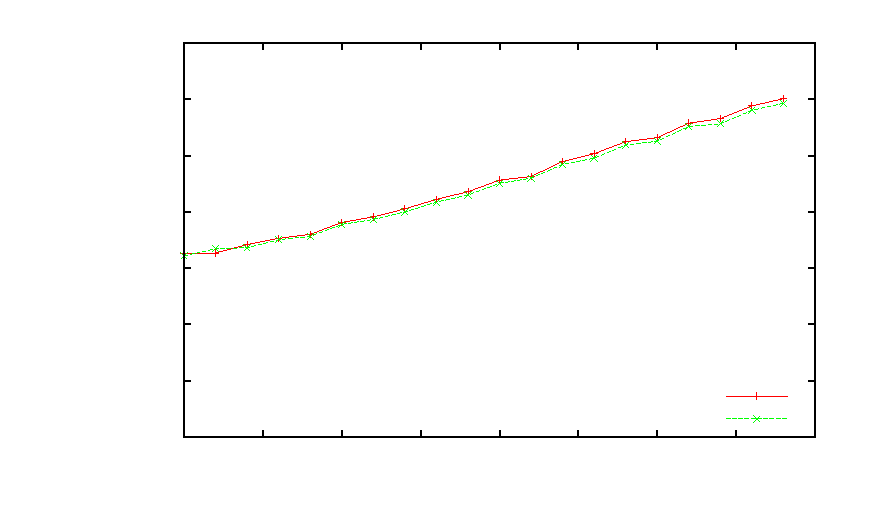
\includegraphics{NaiveVsControlledNodeMemorySkewSelectQuery_L2_DCMrate}}%
    \gplfronttext
  \end{picture}%
\endgroup

	\caption{Level 2 Data Cache Miss Rate}
	\label{fig:NaiveVsControlledNodeMemorySkewSelectQuery_L2_DCMrate}
\end{subfigure}
\hfill
\begin{subfigure}{0.48\textwidth}
	% GNUPLOT: LaTeX picture with Postscript
\begingroup
  \makeatletter
  \providecommand\color[2][]{%
    \GenericError{(gnuplot) \space\space\space\@spaces}{%
      Package color not loaded in conjunction with
      terminal option `colourtext'%
    }{See the gnuplot documentation for explanation.%
    }{Either use 'blacktext' in gnuplot or load the package
      color.sty in LaTeX.}%
    \renewcommand\color[2][]{}%
  }%
  \providecommand\includegraphics[2][]{%
    \GenericError{(gnuplot) \space\space\space\@spaces}{%
      Package graphicx or graphics not loaded%
    }{See the gnuplot documentation for explanation.%
    }{The gnuplot epslatex terminal needs graphicx.sty or graphics.sty.}%
    \renewcommand\includegraphics[2][]{}%
  }%
  \providecommand\rotatebox[2]{#2}%
  \@ifundefined{ifGPcolor}{%
    \newif\ifGPcolor
    \GPcolortrue
  }{}%
  \@ifundefined{ifGPblacktext}{%
    \newif\ifGPblacktext
    \GPblacktexttrue
  }{}%
  % define a \g@addto@macro without @ in the name:
  \let\gplgaddtomacro\g@addto@macro
  % define empty templates for all commands taking text:
  \gdef\gplbacktext{}%
  \gdef\gplfronttext{}%
  \makeatother
  \ifGPblacktext
    % no textcolor at all
    \def\colorrgb#1{}%
    \def\colorgray#1{}%
  \else
    % gray or color?
    \ifGPcolor
      \def\colorrgb#1{\color[rgb]{#1}}%
      \def\colorgray#1{\color[gray]{#1}}%
      \expandafter\def\csname LTw\endcsname{\color{white}}%
      \expandafter\def\csname LTb\endcsname{\color{black}}%
      \expandafter\def\csname LTa\endcsname{\color{black}}%
      \expandafter\def\csname LT0\endcsname{\color[rgb]{1,0,0}}%
      \expandafter\def\csname LT1\endcsname{\color[rgb]{0,1,0}}%
      \expandafter\def\csname LT2\endcsname{\color[rgb]{0,0,1}}%
      \expandafter\def\csname LT3\endcsname{\color[rgb]{1,0,1}}%
      \expandafter\def\csname LT4\endcsname{\color[rgb]{0,1,1}}%
      \expandafter\def\csname LT5\endcsname{\color[rgb]{1,1,0}}%
      \expandafter\def\csname LT6\endcsname{\color[rgb]{0,0,0}}%
      \expandafter\def\csname LT7\endcsname{\color[rgb]{1,0.3,0}}%
      \expandafter\def\csname LT8\endcsname{\color[rgb]{0.5,0.5,0.5}}%
    \else
      % gray
      \def\colorrgb#1{\color{black}}%
      \def\colorgray#1{\color[gray]{#1}}%
      \expandafter\def\csname LTw\endcsname{\color{white}}%
      \expandafter\def\csname LTb\endcsname{\color{black}}%
      \expandafter\def\csname LTa\endcsname{\color{black}}%
      \expandafter\def\csname LT0\endcsname{\color{black}}%
      \expandafter\def\csname LT1\endcsname{\color{black}}%
      \expandafter\def\csname LT2\endcsname{\color{black}}%
      \expandafter\def\csname LT3\endcsname{\color{black}}%
      \expandafter\def\csname LT4\endcsname{\color{black}}%
      \expandafter\def\csname LT5\endcsname{\color{black}}%
      \expandafter\def\csname LT6\endcsname{\color{black}}%
      \expandafter\def\csname LT7\endcsname{\color{black}}%
      \expandafter\def\csname LT8\endcsname{\color{black}}%
    \fi
  \fi
  \setlength{\unitlength}{0.0500bp}%
  \begin{picture}(4608.00,3600.00)%
    \gplgaddtomacro\gplbacktext{%
      \csname LTb\endcsname%
      \put(804,384){\makebox(0,0)[r]{\strut{} 0}}%
      \put(804,823){\makebox(0,0)[r]{\strut{} 200000}}%
      \put(804,1261){\makebox(0,0)[r]{\strut{} 400000}}%
      \put(804,1700){\makebox(0,0)[r]{\strut{} 600000}}%
      \put(804,2139){\makebox(0,0)[r]{\strut{} 800000}}%
      \put(804,2578){\makebox(0,0)[r]{\strut{} 1e+06}}%
      \put(804,3016){\makebox(0,0)[r]{\strut{} 1.2e+06}}%
      \put(804,3455){\makebox(0,0)[r]{\strut{} 1.4e+06}}%
      \put(876,264){\makebox(0,0){\strut{} 2}}%
      \put(1315,264){\makebox(0,0){\strut{} 2.5}}%
      \put(1755,264){\makebox(0,0){\strut{} 3}}%
      \put(2194,264){\makebox(0,0){\strut{} 3.5}}%
      \put(2634,264){\makebox(0,0){\strut{} 4}}%
      \put(3073,264){\makebox(0,0){\strut{} 4.5}}%
      \put(3512,264){\makebox(0,0){\strut{} 5}}%
      \put(3952,264){\makebox(0,0){\strut{} 5.5}}%
      \put(4391,264){\makebox(0,0){\strut{} 6}}%
      \put(96,1919){\rotatebox{-270}{\makebox(0,0){\strut{}TLB}}}%
      \put(2633,84){\makebox(0,0){\strut{}Skew}}%
    }%
    \gplgaddtomacro\gplfronttext{%
      \csname LTb\endcsname%
      \put(3824,3332){\makebox(0,0)[r]{\strut{}NaiveInteger}}%
      \csname LTb\endcsname%
      \put(3824,3212){\makebox(0,0)[r]{\strut{}ControlledMemory}}%
    }%
    \gplbacktext
    \put(0,0){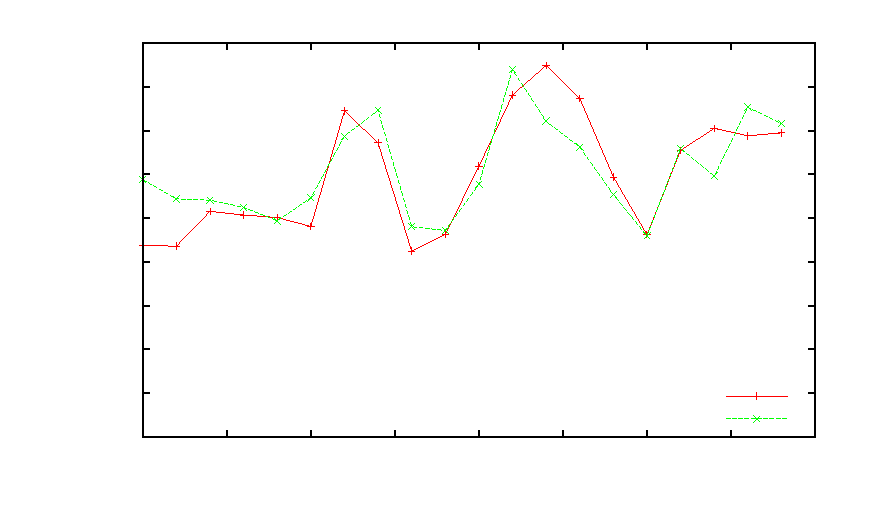
\includegraphics{NaiveVsControlledNodeMemorySkewSelectQueryTLB}}%
    \gplfronttext
  \end{picture}%
\endgroup

	\caption{TLB Misses}
	\label{fig:NaiveVsControlledNodeMemorySkewSelectQueryTLB}
\end{subfigure}

\caption{Various measurements for Select queries on SimpleNaive and ControlledMemory wavelet trees with various skew.}
\label{fig:NaiveVsControlledNodeMemorySkewSelectQuery}

\end{figure}


\restoregeometry
\fi